\documentclass[twoside]{book}

% Packages required by doxygen
\usepackage{calc}
\usepackage{doxygen}
\usepackage{graphicx}
\usepackage[utf8]{inputenc}
\usepackage{makeidx}
\usepackage{multicol}
\usepackage{multirow}
\usepackage{textcomp}
\usepackage[table]{xcolor}

% Font selection
\usepackage[T1]{fontenc}
\usepackage{mathptmx}
\usepackage[scaled=.90]{helvet}
\usepackage{courier}
\usepackage{amssymb}
\usepackage{sectsty}
\renewcommand{\familydefault}{\sfdefault}
\allsectionsfont{%
  \fontseries{bc}\selectfont%
  \color{darkgray}%
}
\renewcommand{\DoxyLabelFont}{%
  \fontseries{bc}\selectfont%
  \color{darkgray}%
}

% Page & text layout
\usepackage{geometry}
\geometry{%
  a4paper,%
  top=2.5cm,%
  bottom=2.5cm,%
  left=2.5cm,%
  right=2.5cm%
}
\tolerance=750
\hfuzz=15pt
\hbadness=750
\setlength{\emergencystretch}{15pt}
\setlength{\parindent}{0cm}
\setlength{\parskip}{0.2cm}
\makeatletter
\renewcommand{\paragraph}{%
  \@startsection{paragraph}{4}{0ex}{-1.0ex}{1.0ex}{%
    \normalfont\normalsize\bfseries\SS@parafont%
  }%
}
\renewcommand{\subparagraph}{%
  \@startsection{subparagraph}{5}{0ex}{-1.0ex}{1.0ex}{%
    \normalfont\normalsize\bfseries\SS@subparafont%
  }%
}
\makeatother

% Headers & footers
\usepackage{fancyhdr}
\pagestyle{fancyplain}
\fancyhead[LE]{\fancyplain{}{\bfseries\thepage}}
\fancyhead[CE]{\fancyplain{}{}}
\fancyhead[RE]{\fancyplain{}{\bfseries\leftmark}}
\fancyhead[LO]{\fancyplain{}{\bfseries\rightmark}}
\fancyhead[CO]{\fancyplain{}{}}
\fancyhead[RO]{\fancyplain{}{\bfseries\thepage}}
\fancyfoot[LE]{\fancyplain{}{}}
\fancyfoot[CE]{\fancyplain{}{}}
\fancyfoot[RE]{\fancyplain{}{\bfseries\scriptsize Generated on Wed Dec 11 2013 03\-:36\-:56 for Physically Based Modeling by Doxygen }}
\fancyfoot[LO]{\fancyplain{}{\bfseries\scriptsize Generated on Wed Dec 11 2013 03\-:36\-:56 for Physically Based Modeling by Doxygen }}
\fancyfoot[CO]{\fancyplain{}{}}
\fancyfoot[RO]{\fancyplain{}{}}
\renewcommand{\footrulewidth}{0.4pt}
\renewcommand{\chaptermark}[1]{%
  \markboth{#1}{}%
}
\renewcommand{\sectionmark}[1]{%
  \markright{\thesection\ #1}%
}

% Indices & bibliography
\usepackage{natbib}
\usepackage[titles]{tocloft}
\setcounter{tocdepth}{3}
\setcounter{secnumdepth}{5}
\makeindex

% Hyperlinks (required, but should be loaded last)
\usepackage{ifpdf}
\ifpdf
  \usepackage[pdftex,pagebackref=true]{hyperref}
\else
  \usepackage[ps2pdf,pagebackref=true]{hyperref}
\fi
\hypersetup{%
  colorlinks=true,%
  linkcolor=blue,%
  citecolor=blue,%
  unicode%
}

% Custom commands
\newcommand{\clearemptydoublepage}{%
  \newpage{\pagestyle{empty}\cleardoublepage}%
}


%===== C O N T E N T S =====

\begin{document}

% Titlepage & ToC
\hypersetup{pageanchor=false}
\pagenumbering{roman}
\begin{titlepage}
\vspace*{7cm}
\begin{center}%
{\Large Physically Based Modeling }\\
\vspace*{1cm}
{\large Generated by Doxygen 1.8.5}\\
\vspace*{0.5cm}
{\small Wed Dec 11 2013 03:36:56}\\
\end{center}
\end{titlepage}
\clearemptydoublepage
\tableofcontents
\clearemptydoublepage
\pagenumbering{arabic}
\hypersetup{pageanchor=true}

%--- Begin generated contents ---
\chapter{Namespace Index}
\section{Namespace List}
Here is a list of all namespaces with brief descriptions\-:\begin{DoxyCompactList}
\item\contentsline{section}{\hyperlink{namespace_collision_handler}{Collision\-Handler} }{\pageref{namespace_collision_handler}}{}
\item\contentsline{section}{\hyperlink{namespace_ui}{Ui} }{\pageref{namespace_ui}}{}
\end{DoxyCompactList}

\chapter{Hierarchical Index}
\section{Class Hierarchy}
This inheritance list is sorted roughly, but not completely, alphabetically\-:\begin{DoxyCompactList}
\item \contentsline{section}{Collision\-Force}{\pageref{class_collision_force}}{}
\item \contentsline{section}{Deferred\-Force}{\pageref{class_deferred_force}}{}
\begin{DoxyCompactList}
\item \contentsline{section}{R\-B\-Deferred\-Force}{\pageref{class_r_b_deferred_force}}{}
\item \contentsline{section}{Simple\-Deferred\-Force}{\pageref{class_simple_deferred_force}}{}
\end{DoxyCompactList}
\item \contentsline{section}{Environment}{\pageref{class_environment}}{}
\item \contentsline{section}{Force}{\pageref{class_force}}{}
\begin{DoxyCompactList}
\item \contentsline{section}{Independent\-Force}{\pageref{class_independent_force}}{}
\end{DoxyCompactList}
\item \contentsline{section}{Force\-Environment}{\pageref{class_force_environment}}{}
\item \contentsline{section}{Hi\-Def\-Color}{\pageref{class_hi_def_color}}{}
\item \contentsline{section}{Matrix3\-D}{\pageref{class_matrix3_d}}{}
\item \contentsline{section}{Object}{\pageref{class_object}}{}
\begin{DoxyCompactList}
\item \contentsline{section}{Collidable\-Object}{\pageref{class_collidable_object}}{}
\begin{DoxyCompactList}
\item \contentsline{section}{Collider\-Object}{\pageref{class_collider_object}}{}
\item \contentsline{section}{Physical}{\pageref{class_physical}}{}
\begin{DoxyCompactList}
\item \contentsline{section}{Rigid\-Body}{\pageref{class_rigid_body}}{}
\end{DoxyCompactList}
\end{DoxyCompactList}
\end{DoxyCompactList}
\item \contentsline{section}{P\-B\-Time}{\pageref{class_p_b_time}}{}
\item Q\-Event\begin{DoxyCompactList}
\item \contentsline{section}{Phys\-B\-Event}{\pageref{class_phys_b_event}}{}
\end{DoxyCompactList}
\item Q\-Main\-Window\begin{DoxyCompactList}
\item \contentsline{section}{Application}{\pageref{class_application}}{}
\end{DoxyCompactList}
\item Q\-Widget\begin{DoxyCompactList}
\item \contentsline{section}{Q\-S\-F\-M\-L\-Canvas}{\pageref{class_q_s_f_m_l_canvas}}{}
\end{DoxyCompactList}
\item \contentsline{section}{Renderable}{\pageref{class_renderable}}{}
\begin{DoxyCompactList}
\item \contentsline{section}{Shape}{\pageref{class_shape}}{}
\begin{DoxyCompactList}
\item \contentsline{section}{Box}{\pageref{class_box}}{}
\item \contentsline{section}{Quad\-Plane}{\pageref{class_quad_plane}}{}
\item \contentsline{section}{Sphere}{\pageref{class_sphere}}{}
\end{DoxyCompactList}
\end{DoxyCompactList}
\item Render\-Window\begin{DoxyCompactList}
\item \contentsline{section}{R\-W\-Wrapper}{\pageref{class_r_w_wrapper}}{}
\begin{DoxyCompactList}
\item \contentsline{section}{Q\-S\-F\-M\-L\-Canvas}{\pageref{class_q_s_f_m_l_canvas}}{}
\end{DoxyCompactList}
\end{DoxyCompactList}
\item \contentsline{section}{Transform}{\pageref{class_transform}}{}
\item \contentsline{section}{Ui\-\_\-\-Phys\-B\-Dock}{\pageref{class_ui___phys_b_dock}}{}
\begin{DoxyCompactList}
\item \contentsline{section}{Ui\-:\-:Phys\-B\-Dock}{\pageref{class_ui_1_1_phys_b_dock}}{}
\end{DoxyCompactList}
\item \contentsline{section}{Vector2\-D}{\pageref{class_vector2_d}}{}
\item \contentsline{section}{Vector3\-D}{\pageref{class_vector3_d}}{}
\end{DoxyCompactList}

\chapter{Class Index}
\section{Class List}
Here are the classes, structs, unions and interfaces with brief descriptions\-:\begin{DoxyCompactList}
\item\contentsline{section}{\hyperlink{class_application}{Application} }{\pageref{class_application}}{}
\item\contentsline{section}{\hyperlink{class_box}{Box} }{\pageref{class_box}}{}
\item\contentsline{section}{\hyperlink{class_collidable_object}{Collidable\-Object} }{\pageref{class_collidable_object}}{}
\item\contentsline{section}{\hyperlink{class_collider_object}{Collider\-Object} }{\pageref{class_collider_object}}{}
\item\contentsline{section}{\hyperlink{class_collision_force}{Collision\-Force} }{\pageref{class_collision_force}}{}
\item\contentsline{section}{\hyperlink{class_deferred_force}{Deferred\-Force} }{\pageref{class_deferred_force}}{}
\item\contentsline{section}{\hyperlink{class_environment}{Environment} }{\pageref{class_environment}}{}
\item\contentsline{section}{\hyperlink{class_force}{Force} }{\pageref{class_force}}{}
\item\contentsline{section}{\hyperlink{class_force_environment}{Force\-Environment} }{\pageref{class_force_environment}}{}
\item\contentsline{section}{\hyperlink{class_hi_def_color}{Hi\-Def\-Color} }{\pageref{class_hi_def_color}}{}
\item\contentsline{section}{\hyperlink{class_independent_force}{Independent\-Force} }{\pageref{class_independent_force}}{}
\item\contentsline{section}{\hyperlink{class_matrix3_d}{Matrix3\-D} }{\pageref{class_matrix3_d}}{}
\item\contentsline{section}{\hyperlink{class_object}{Object} }{\pageref{class_object}}{}
\item\contentsline{section}{\hyperlink{class_p_b_time}{P\-B\-Time} }{\pageref{class_p_b_time}}{}
\item\contentsline{section}{\hyperlink{class_ui_1_1_phys_b_dock}{Ui\-::\-Phys\-B\-Dock} }{\pageref{class_ui_1_1_phys_b_dock}}{}
\item\contentsline{section}{\hyperlink{class_phys_b_event}{Phys\-B\-Event} }{\pageref{class_phys_b_event}}{}
\item\contentsline{section}{\hyperlink{class_physical}{Physical} }{\pageref{class_physical}}{}
\item\contentsline{section}{\hyperlink{class_q_s_f_m_l_canvas}{Q\-S\-F\-M\-L\-Canvas} }{\pageref{class_q_s_f_m_l_canvas}}{}
\item\contentsline{section}{\hyperlink{class_quad_plane}{Quad\-Plane} }{\pageref{class_quad_plane}}{}
\item\contentsline{section}{\hyperlink{class_r_b_deferred_force}{R\-B\-Deferred\-Force} }{\pageref{class_r_b_deferred_force}}{}
\item\contentsline{section}{\hyperlink{class_renderable}{Renderable} }{\pageref{class_renderable}}{}
\item\contentsline{section}{\hyperlink{class_rigid_body}{Rigid\-Body} }{\pageref{class_rigid_body}}{}
\item\contentsline{section}{\hyperlink{class_r_w_wrapper}{R\-W\-Wrapper} }{\pageref{class_r_w_wrapper}}{}
\item\contentsline{section}{\hyperlink{class_shape}{Shape} }{\pageref{class_shape}}{}
\item\contentsline{section}{\hyperlink{class_simple_deferred_force}{Simple\-Deferred\-Force} }{\pageref{class_simple_deferred_force}}{}
\item\contentsline{section}{\hyperlink{class_sphere}{Sphere} }{\pageref{class_sphere}}{}
\item\contentsline{section}{\hyperlink{class_transform}{Transform} }{\pageref{class_transform}}{}
\item\contentsline{section}{\hyperlink{class_ui___phys_b_dock}{Ui\-\_\-\-Phys\-B\-Dock} }{\pageref{class_ui___phys_b_dock}}{}
\item\contentsline{section}{\hyperlink{class_vector2_d}{Vector2\-D} }{\pageref{class_vector2_d}}{}
\item\contentsline{section}{\hyperlink{class_vector3_d}{Vector3\-D} }{\pageref{class_vector3_d}}{}
\end{DoxyCompactList}

\chapter{File Index}
\section{File List}
Here is a list of all files with brief descriptions\-:\begin{DoxyCompactList}
\item\contentsline{section}{D\-:/\-Development/\-My\-Projects/\-Physically\-Based\-Modeling/include/\hyperlink{_application_8h}{Application.\-h} }{\pageref{_application_8h}}{}
\item\contentsline{section}{D\-:/\-Development/\-My\-Projects/\-Physically\-Based\-Modeling/include/\hyperlink{_box_8h}{Box.\-h} }{\pageref{_box_8h}}{}
\item\contentsline{section}{D\-:/\-Development/\-My\-Projects/\-Physically\-Based\-Modeling/include/\hyperlink{_collidable_object_8h}{Collidable\-Object.\-h} }{\pageref{_collidable_object_8h}}{}
\item\contentsline{section}{D\-:/\-Development/\-My\-Projects/\-Physically\-Based\-Modeling/include/\hyperlink{_collider_object_8h}{Collider\-Object.\-h} }{\pageref{_collider_object_8h}}{}
\item\contentsline{section}{D\-:/\-Development/\-My\-Projects/\-Physically\-Based\-Modeling/include/\hyperlink{_collision_handler_8h}{Collision\-Handler.\-h} }{\pageref{_collision_handler_8h}}{}
\item\contentsline{section}{D\-:/\-Development/\-My\-Projects/\-Physically\-Based\-Modeling/include/\hyperlink{_environment_8h}{Environment.\-h} }{\pageref{_environment_8h}}{}
\item\contentsline{section}{D\-:/\-Development/\-My\-Projects/\-Physically\-Based\-Modeling/include/\hyperlink{_events_8h}{Events.\-h} }{\pageref{_events_8h}}{}
\item\contentsline{section}{D\-:/\-Development/\-My\-Projects/\-Physically\-Based\-Modeling/include/\hyperlink{_force_8h}{Force.\-h} }{\pageref{_force_8h}}{}
\item\contentsline{section}{D\-:/\-Development/\-My\-Projects/\-Physically\-Based\-Modeling/include/\hyperlink{_force_environment_8h}{Force\-Environment.\-h} }{\pageref{_force_environment_8h}}{}
\item\contentsline{section}{D\-:/\-Development/\-My\-Projects/\-Physically\-Based\-Modeling/include/\hyperlink{_object_8h}{Object.\-h} }{\pageref{_object_8h}}{}
\item\contentsline{section}{D\-:/\-Development/\-My\-Projects/\-Physically\-Based\-Modeling/include/\hyperlink{_physical_8h}{Physical.\-h} }{\pageref{_physical_8h}}{}
\item\contentsline{section}{D\-:/\-Development/\-My\-Projects/\-Physically\-Based\-Modeling/include/\hyperlink{_physically_based_8h}{Physically\-Based.\-h} }{\pageref{_physically_based_8h}}{}
\item\contentsline{section}{D\-:/\-Development/\-My\-Projects/\-Physically\-Based\-Modeling/include/\hyperlink{_quad_plane_8h}{Quad\-Plane.\-h} }{\pageref{_quad_plane_8h}}{}
\item\contentsline{section}{D\-:/\-Development/\-My\-Projects/\-Physically\-Based\-Modeling/include/\hyperlink{_renderable_8h}{Renderable.\-h} }{\pageref{_renderable_8h}}{}
\item\contentsline{section}{D\-:/\-Development/\-My\-Projects/\-Physically\-Based\-Modeling/include/\hyperlink{_rigid_body_8h}{Rigid\-Body.\-h} }{\pageref{_rigid_body_8h}}{}
\item\contentsline{section}{D\-:/\-Development/\-My\-Projects/\-Physically\-Based\-Modeling/include/\hyperlink{_shape_8h}{Shape.\-h} }{\pageref{_shape_8h}}{}
\item\contentsline{section}{D\-:/\-Development/\-My\-Projects/\-Physically\-Based\-Modeling/include/\hyperlink{_sphere_8h}{Sphere.\-h} }{\pageref{_sphere_8h}}{}
\item\contentsline{section}{D\-:/\-Development/\-My\-Projects/\-Physically\-Based\-Modeling/include/\hyperlink{_transform_8h}{Transform.\-h} }{\pageref{_transform_8h}}{}
\item\contentsline{section}{D\-:/\-Development/\-My\-Projects/\-Physically\-Based\-Modeling/include/\hyperlink{ui___physically_based_8h}{ui\-\_\-\-Physically\-Based.\-h} }{\pageref{ui___physically_based_8h}}{}
\item\contentsline{section}{D\-:/\-Development/\-My\-Projects/\-Physically\-Based\-Modeling/include/\hyperlink{_utility_8h}{Utility.\-h} }{\pageref{_utility_8h}}{}
\item\contentsline{section}{D\-:/\-Development/\-My\-Projects/\-Physically\-Based\-Modeling/include/\-G\-U\-I/\hyperlink{_q_s_f_m_l_canvas_8h}{Q\-S\-F\-M\-L\-Canvas.\-h} }{\pageref{_q_s_f_m_l_canvas_8h}}{}
\item\contentsline{section}{D\-:/\-Development/\-My\-Projects/\-Physically\-Based\-Modeling/include/\-G\-U\-I/\hyperlink{render_window_wrapper_8h}{render\-Window\-Wrapper.\-h} }{\pageref{render_window_wrapper_8h}}{}
\end{DoxyCompactList}

\chapter{Namespace Documentation}
\hypertarget{namespace_collision_handler}{\section{Collision\-Handler Namespace Reference}
\label{namespace_collision_handler}\index{Collision\-Handler@{Collision\-Handler}}
}
\subsection*{Functions}
\begin{DoxyCompactItemize}
\item 
bool \hyperlink{namespace_collision_handler_a745096d27ac0c37c74f82334184b73db}{collision} (const \hyperlink{class_quad_plane}{Quad\-Plane} \&qp, const \hyperlink{class_transform}{Transform} \&qp\-\_\-new\-Tr, const \hyperlink{class_sphere}{Sphere} \&s, const \hyperlink{class_transform}{Transform} \&s\-\_\-new\-Tr, float $\ast$timestep\-Frac, \hyperlink{class_vector3_d}{Vector3\-D} $\ast$collision\-Normal)
\item 
bool \hyperlink{namespace_collision_handler_abdf4d543db8d5f6fc012ff91f31f2140}{collision} (const \hyperlink{class_sphere}{Sphere} \&s, const \hyperlink{class_vector3_d}{Vector3\-D} \&s\-\_\-p0, const \hyperlink{class_vector3_d}{Vector3\-D} \&s\-\_\-p1, const \hyperlink{class_quad_plane}{Quad\-Plane} \&qp, const \hyperlink{class_vector3_d}{Vector3\-D} \&qp\-\_\-p0, const \hyperlink{class_vector3_d}{Vector3\-D} \&qp\-\_\-p1, float $\ast$timestep\-Frac, \hyperlink{class_vector3_d}{Vector3\-D} $\ast$collision\-Normal)
\item 
bool \hyperlink{namespace_collision_handler_a1bfa74edc99009c5e18c44df30ead02f}{collision} (const \hyperlink{class_sphere}{Sphere} \&s0, const \hyperlink{class_vector3_d}{Vector3\-D} \&s0\-\_\-p0, const \hyperlink{class_vector3_d}{Vector3\-D} \&s0\-\_\-p1, const \hyperlink{class_sphere}{Sphere} \&s1, const \hyperlink{class_vector3_d}{Vector3\-D} \&s1\-\_\-p0, const \hyperlink{class_vector3_d}{Vector3\-D} \&s1\-\_\-p1, float $\ast$timestep\-Frac, \hyperlink{class_vector3_d}{Vector3\-D} $\ast$collision\-Normal)
\item 
bool \hyperlink{namespace_collision_handler_ac02fa6575701dd41985e32674370dbf2}{collision} (const \hyperlink{class_quad_plane}{Quad\-Plane} \&s0, const \hyperlink{class_vector3_d}{Vector3\-D} \&qp0\-\_\-p0, const \hyperlink{class_vector3_d}{Vector3\-D} \&qp0\-\_\-p1, const \hyperlink{class_quad_plane}{Quad\-Plane} \&s1, const \hyperlink{class_vector3_d}{Vector3\-D} \&qp1\-\_\-p0, const \hyperlink{class_vector3_d}{Vector3\-D} \&qp1\-\_\-p1, float $\ast$timestep\-Frac, \hyperlink{class_vector3_d}{Vector3\-D} $\ast$collision\-Normal)
\end{DoxyCompactItemize}


\subsection{Function Documentation}
\hypertarget{namespace_collision_handler_a745096d27ac0c37c74f82334184b73db}{\index{Collision\-Handler@{Collision\-Handler}!collision@{collision}}
\index{collision@{collision}!CollisionHandler@{Collision\-Handler}}
\subsubsection[{collision}]{\setlength{\rightskip}{0pt plus 5cm}bool Collision\-Handler\-::collision (
\begin{DoxyParamCaption}
\item[{const {\bf Quad\-Plane} \&}]{qp, }
\item[{const {\bf Transform} \&}]{qp\-\_\-new\-Tr, }
\item[{const {\bf Sphere} \&}]{s, }
\item[{const {\bf Transform} \&}]{s\-\_\-new\-Tr, }
\item[{float $\ast$}]{timestep\-Frac, }
\item[{{\bf Vector3\-D} $\ast$}]{collision\-Normal}
\end{DoxyParamCaption}
)}}\label{namespace_collision_handler_a745096d27ac0c37c74f82334184b73db}
\hypertarget{namespace_collision_handler_abdf4d543db8d5f6fc012ff91f31f2140}{\index{Collision\-Handler@{Collision\-Handler}!collision@{collision}}
\index{collision@{collision}!CollisionHandler@{Collision\-Handler}}
\subsubsection[{collision}]{\setlength{\rightskip}{0pt plus 5cm}bool Collision\-Handler\-::collision (
\begin{DoxyParamCaption}
\item[{const {\bf Sphere} \&}]{s, }
\item[{const {\bf Vector3\-D} \&}]{s\-\_\-p0, }
\item[{const {\bf Vector3\-D} \&}]{s\-\_\-p1, }
\item[{const {\bf Quad\-Plane} \&}]{qp, }
\item[{const {\bf Vector3\-D} \&}]{qp\-\_\-p0, }
\item[{const {\bf Vector3\-D} \&}]{qp\-\_\-p1, }
\item[{float $\ast$}]{timestep\-Frac, }
\item[{{\bf Vector3\-D} $\ast$}]{collision\-Normal}
\end{DoxyParamCaption}
)}}\label{namespace_collision_handler_abdf4d543db8d5f6fc012ff91f31f2140}
\hypertarget{namespace_collision_handler_a1bfa74edc99009c5e18c44df30ead02f}{\index{Collision\-Handler@{Collision\-Handler}!collision@{collision}}
\index{collision@{collision}!CollisionHandler@{Collision\-Handler}}
\subsubsection[{collision}]{\setlength{\rightskip}{0pt plus 5cm}bool Collision\-Handler\-::collision (
\begin{DoxyParamCaption}
\item[{const {\bf Sphere} \&}]{s0, }
\item[{const {\bf Vector3\-D} \&}]{s0\-\_\-p0, }
\item[{const {\bf Vector3\-D} \&}]{s0\-\_\-p1, }
\item[{const {\bf Sphere} \&}]{s1, }
\item[{const {\bf Vector3\-D} \&}]{s1\-\_\-p0, }
\item[{const {\bf Vector3\-D} \&}]{s1\-\_\-p1, }
\item[{float $\ast$}]{timestep\-Frac, }
\item[{{\bf Vector3\-D} $\ast$}]{collision\-Normal}
\end{DoxyParamCaption}
)}}\label{namespace_collision_handler_a1bfa74edc99009c5e18c44df30ead02f}
\hypertarget{namespace_collision_handler_ac02fa6575701dd41985e32674370dbf2}{\index{Collision\-Handler@{Collision\-Handler}!collision@{collision}}
\index{collision@{collision}!CollisionHandler@{Collision\-Handler}}
\subsubsection[{collision}]{\setlength{\rightskip}{0pt plus 5cm}bool Collision\-Handler\-::collision (
\begin{DoxyParamCaption}
\item[{const {\bf Quad\-Plane} \&}]{s0, }
\item[{const {\bf Vector3\-D} \&}]{qp0\-\_\-p0, }
\item[{const {\bf Vector3\-D} \&}]{qp0\-\_\-p1, }
\item[{const {\bf Quad\-Plane} \&}]{s1, }
\item[{const {\bf Vector3\-D} \&}]{qp1\-\_\-p0, }
\item[{const {\bf Vector3\-D} \&}]{qp1\-\_\-p1, }
\item[{float $\ast$}]{timestep\-Frac, }
\item[{{\bf Vector3\-D} $\ast$}]{collision\-Normal}
\end{DoxyParamCaption}
)}}\label{namespace_collision_handler_ac02fa6575701dd41985e32674370dbf2}

\hypertarget{namespace_ui}{\section{Ui Namespace Reference}
\label{namespace_ui}\index{Ui@{Ui}}
}
\subsection*{Classes}
\begin{DoxyCompactItemize}
\item 
class \hyperlink{class_ui_1_1_phys_b_dock}{Phys\-B\-Dock}
\end{DoxyCompactItemize}

\chapter{Class Documentation}
\hypertarget{class_application}{\section{Application Class Reference}
\label{class_application}\index{Application@{Application}}
}


{\ttfamily \#include $<$Application.\-h$>$}

Inheritance diagram for Application\-:\begin{figure}[H]
\begin{center}
\leavevmode
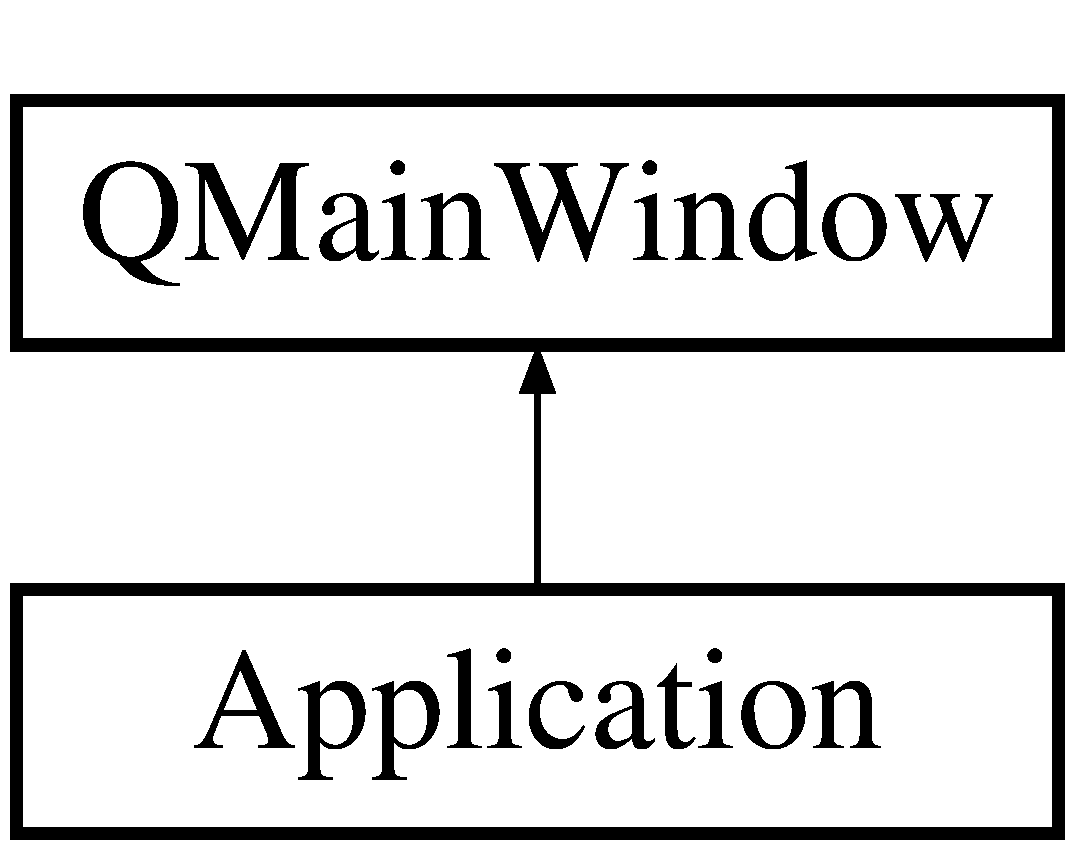
\includegraphics[height=2.000000cm]{class_application}
\end{center}
\end{figure}
\subsection*{Public Member Functions}
\begin{DoxyCompactItemize}
\item 
\hyperlink{class_application_a748bca84fefb9c12661cfaa2f623748d}{$\sim$\-Application} ()
\end{DoxyCompactItemize}
\subsection*{Static Public Member Functions}
\begin{DoxyCompactItemize}
\item 
static void \hyperlink{class_application_a8eb19fef68c6c556f069ab894192ad8c}{create} (std\-::string assets)
\item 
static \hyperlink{class_application}{Application} $\ast$ \hyperlink{class_application_ab5dba709d2e806d5d83c297bab6cdace}{get\-Instance} ()
\end{DoxyCompactItemize}
\subsection*{Protected Member Functions}
\begin{DoxyCompactItemize}
\item 
void \hyperlink{class_application_a0170cac84e135e75e3177ed2d185ba0a}{close\-Event} (Q\-Close\-Event $\ast$event)
\item 
void \hyperlink{class_application_a3151617f344f6a246ba47b6db79c3778}{custom\-Event} (Q\-Event $\ast$event)
\end{DoxyCompactItemize}
\subsection*{Friends}
\begin{DoxyCompactItemize}
\item 
class \hyperlink{class_application_aeee6bd23afed3d408fb21a7d857a8f3b}{Physically\-Based}
\end{DoxyCompactItemize}


\subsection{Constructor \& Destructor Documentation}
\hypertarget{class_application_a748bca84fefb9c12661cfaa2f623748d}{\index{Application@{Application}!$\sim$\-Application@{$\sim$\-Application}}
\index{$\sim$\-Application@{$\sim$\-Application}!Application@{Application}}
\subsubsection[{$\sim$\-Application}]{\setlength{\rightskip}{0pt plus 5cm}Application\-::$\sim$\-Application (
\begin{DoxyParamCaption}
{}
\end{DoxyParamCaption}
)\hspace{0.3cm}{\ttfamily [inline]}}}\label{class_application_a748bca84fefb9c12661cfaa2f623748d}


\subsection{Member Function Documentation}
\hypertarget{class_application_a0170cac84e135e75e3177ed2d185ba0a}{\index{Application@{Application}!close\-Event@{close\-Event}}
\index{close\-Event@{close\-Event}!Application@{Application}}
\subsubsection[{close\-Event}]{\setlength{\rightskip}{0pt plus 5cm}void Application\-::close\-Event (
\begin{DoxyParamCaption}
\item[{Q\-Close\-Event $\ast$}]{event}
\end{DoxyParamCaption}
)\hspace{0.3cm}{\ttfamily [protected]}}}\label{class_application_a0170cac84e135e75e3177ed2d185ba0a}
\hypertarget{class_application_a8eb19fef68c6c556f069ab894192ad8c}{\index{Application@{Application}!create@{create}}
\index{create@{create}!Application@{Application}}
\subsubsection[{create}]{\setlength{\rightskip}{0pt plus 5cm}static void Application\-::create (
\begin{DoxyParamCaption}
\item[{std\-::string}]{assets}
\end{DoxyParamCaption}
)\hspace{0.3cm}{\ttfamily [static]}}}\label{class_application_a8eb19fef68c6c556f069ab894192ad8c}
\hypertarget{class_application_a3151617f344f6a246ba47b6db79c3778}{\index{Application@{Application}!custom\-Event@{custom\-Event}}
\index{custom\-Event@{custom\-Event}!Application@{Application}}
\subsubsection[{custom\-Event}]{\setlength{\rightskip}{0pt plus 5cm}void Application\-::custom\-Event (
\begin{DoxyParamCaption}
\item[{Q\-Event $\ast$}]{event}
\end{DoxyParamCaption}
)\hspace{0.3cm}{\ttfamily [protected]}}}\label{class_application_a3151617f344f6a246ba47b6db79c3778}
\hypertarget{class_application_ab5dba709d2e806d5d83c297bab6cdace}{\index{Application@{Application}!get\-Instance@{get\-Instance}}
\index{get\-Instance@{get\-Instance}!Application@{Application}}
\subsubsection[{get\-Instance}]{\setlength{\rightskip}{0pt plus 5cm}static {\bf Application}$\ast$ Application\-::get\-Instance (
\begin{DoxyParamCaption}
{}
\end{DoxyParamCaption}
)\hspace{0.3cm}{\ttfamily [static]}}}\label{class_application_ab5dba709d2e806d5d83c297bab6cdace}


\subsection{Friends And Related Function Documentation}
\hypertarget{class_application_aeee6bd23afed3d408fb21a7d857a8f3b}{\index{Application@{Application}!Physically\-Based@{Physically\-Based}}
\index{Physically\-Based@{Physically\-Based}!Application@{Application}}
\subsubsection[{Physically\-Based}]{\setlength{\rightskip}{0pt plus 5cm}friend class Physically\-Based\hspace{0.3cm}{\ttfamily [friend]}}}\label{class_application_aeee6bd23afed3d408fb21a7d857a8f3b}


The documentation for this class was generated from the following file\-:\begin{DoxyCompactItemize}
\item 
D\-:/\-Development/\-My\-Projects/\-Physically\-Based\-Modeling/include/\hyperlink{_application_8h}{Application.\-h}\end{DoxyCompactItemize}

\hypertarget{class_box}{\section{Box Class Reference}
\label{class_box}\index{Box@{Box}}
}


{\ttfamily \#include $<$Box.\-h$>$}

Inheritance diagram for Box\-:\begin{figure}[H]
\begin{center}
\leavevmode
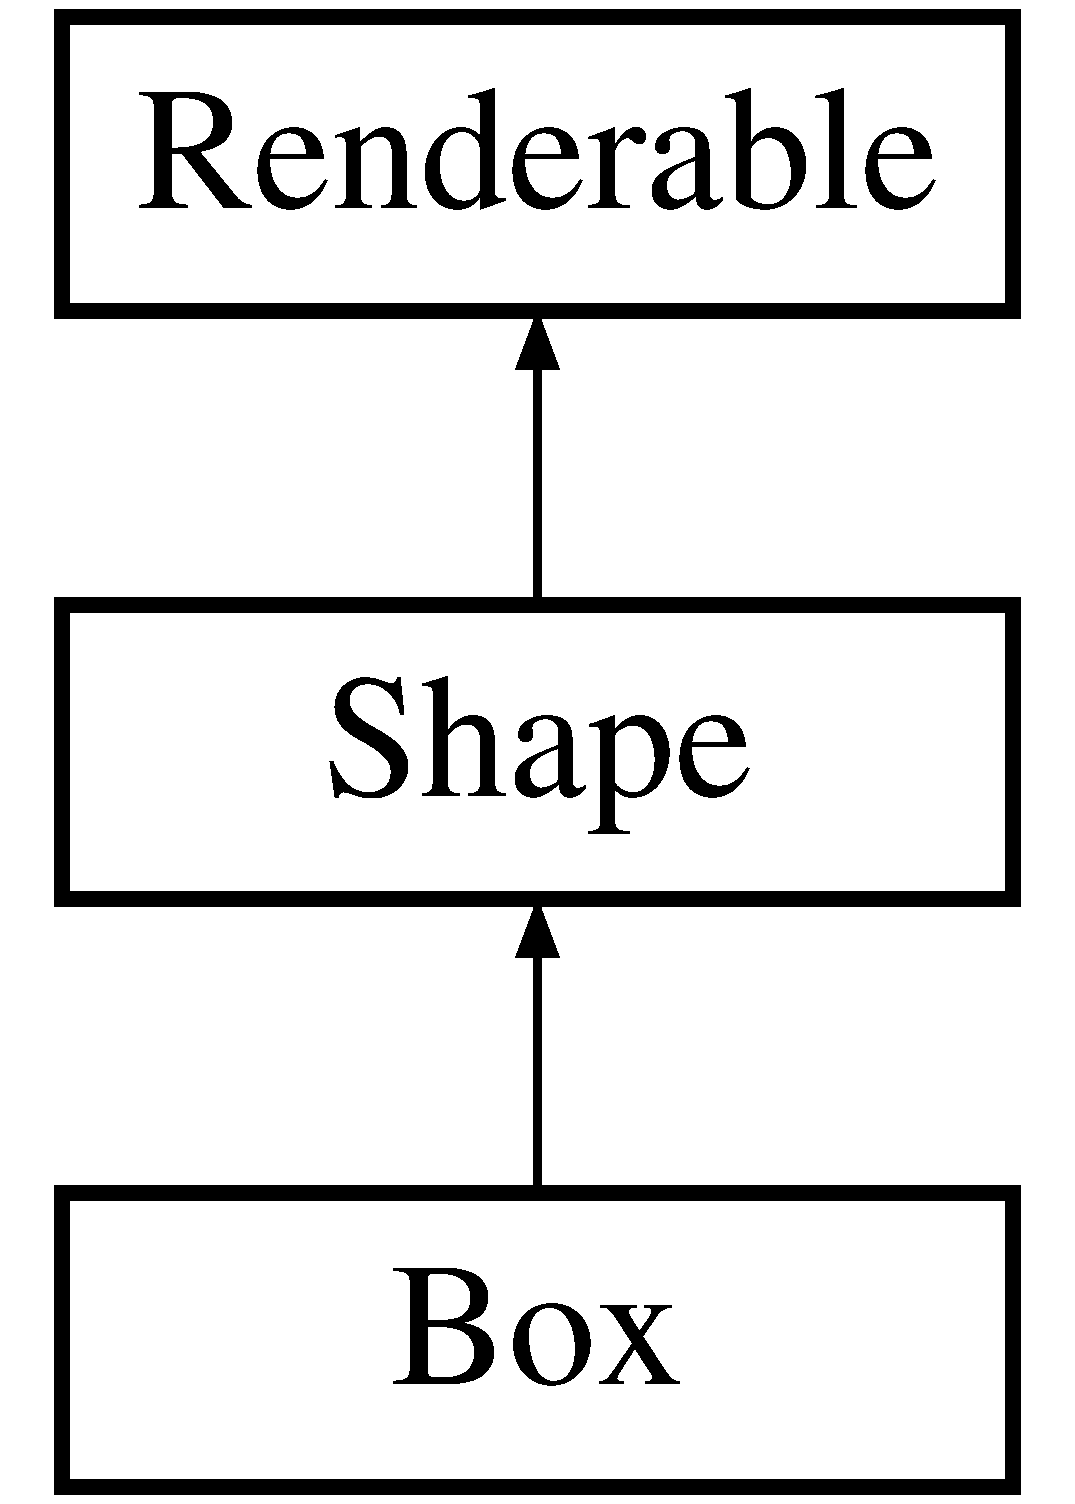
\includegraphics[height=3.000000cm]{class_box}
\end{center}
\end{figure}
\subsection*{Public Member Functions}
\begin{DoxyCompactItemize}
\item 
\hyperlink{class_box_a7fa11ba4e964762f032e71e817d31675}{Box} (const \hyperlink{class_vector3_d}{Vector3\-D} \&dimensions, const \hyperlink{class_vector3_d}{Vector3\-D} \&pos, std\-::string name)
\item 
\hyperlink{class_vector3_d}{Vector3\-D} \hyperlink{class_box_ad975c9186f66278e3697367885616bdc}{get\-Dim} () const 
\item 
float \hyperlink{class_box_aa09a0a9386e4e6253cae093a3d4a7ce7}{get\-Width} () const 
\item 
float \hyperlink{class_box_ae5bf643fcf1d32d03d503f4bded3ea2a}{get\-Height} () const 
\item 
float \hyperlink{class_box_aef027760b7966d479353b05b7e886210}{get\-Depth} () const 
\end{DoxyCompactItemize}
\subsection*{Additional Inherited Members}


\subsection{Constructor \& Destructor Documentation}
\hypertarget{class_box_a7fa11ba4e964762f032e71e817d31675}{\index{Box@{Box}!Box@{Box}}
\index{Box@{Box}!Box@{Box}}
\subsubsection[{Box}]{\setlength{\rightskip}{0pt plus 5cm}Box\-::\-Box (
\begin{DoxyParamCaption}
\item[{const {\bf Vector3\-D} \&}]{dimensions, }
\item[{const {\bf Vector3\-D} \&}]{pos, }
\item[{std\-::string}]{name}
\end{DoxyParamCaption}
)\hspace{0.3cm}{\ttfamily [inline]}}}\label{class_box_a7fa11ba4e964762f032e71e817d31675}


\subsection{Member Function Documentation}
\hypertarget{class_box_aef027760b7966d479353b05b7e886210}{\index{Box@{Box}!get\-Depth@{get\-Depth}}
\index{get\-Depth@{get\-Depth}!Box@{Box}}
\subsubsection[{get\-Depth}]{\setlength{\rightskip}{0pt plus 5cm}float Box\-::get\-Depth (
\begin{DoxyParamCaption}
{}
\end{DoxyParamCaption}
) const\hspace{0.3cm}{\ttfamily [inline]}}}\label{class_box_aef027760b7966d479353b05b7e886210}
\hypertarget{class_box_ad975c9186f66278e3697367885616bdc}{\index{Box@{Box}!get\-Dim@{get\-Dim}}
\index{get\-Dim@{get\-Dim}!Box@{Box}}
\subsubsection[{get\-Dim}]{\setlength{\rightskip}{0pt plus 5cm}{\bf Vector3\-D} Box\-::get\-Dim (
\begin{DoxyParamCaption}
{}
\end{DoxyParamCaption}
) const\hspace{0.3cm}{\ttfamily [inline]}}}\label{class_box_ad975c9186f66278e3697367885616bdc}
\hypertarget{class_box_ae5bf643fcf1d32d03d503f4bded3ea2a}{\index{Box@{Box}!get\-Height@{get\-Height}}
\index{get\-Height@{get\-Height}!Box@{Box}}
\subsubsection[{get\-Height}]{\setlength{\rightskip}{0pt plus 5cm}float Box\-::get\-Height (
\begin{DoxyParamCaption}
{}
\end{DoxyParamCaption}
) const\hspace{0.3cm}{\ttfamily [inline]}}}\label{class_box_ae5bf643fcf1d32d03d503f4bded3ea2a}
\hypertarget{class_box_aa09a0a9386e4e6253cae093a3d4a7ce7}{\index{Box@{Box}!get\-Width@{get\-Width}}
\index{get\-Width@{get\-Width}!Box@{Box}}
\subsubsection[{get\-Width}]{\setlength{\rightskip}{0pt plus 5cm}float Box\-::get\-Width (
\begin{DoxyParamCaption}
{}
\end{DoxyParamCaption}
) const\hspace{0.3cm}{\ttfamily [inline]}}}\label{class_box_aa09a0a9386e4e6253cae093a3d4a7ce7}


The documentation for this class was generated from the following file\-:\begin{DoxyCompactItemize}
\item 
D\-:/\-Development/\-My\-Projects/\-Physically\-Based\-Modeling/include/\hyperlink{_box_8h}{Box.\-h}\end{DoxyCompactItemize}

\hypertarget{class_collidable_object}{\section{Collidable\-Object Class Reference}
\label{class_collidable_object}\index{Collidable\-Object@{Collidable\-Object}}
}


{\ttfamily \#include $<$Collidable\-Object.\-h$>$}

Inheritance diagram for Collidable\-Object\-:\begin{figure}[H]
\begin{center}
\leavevmode
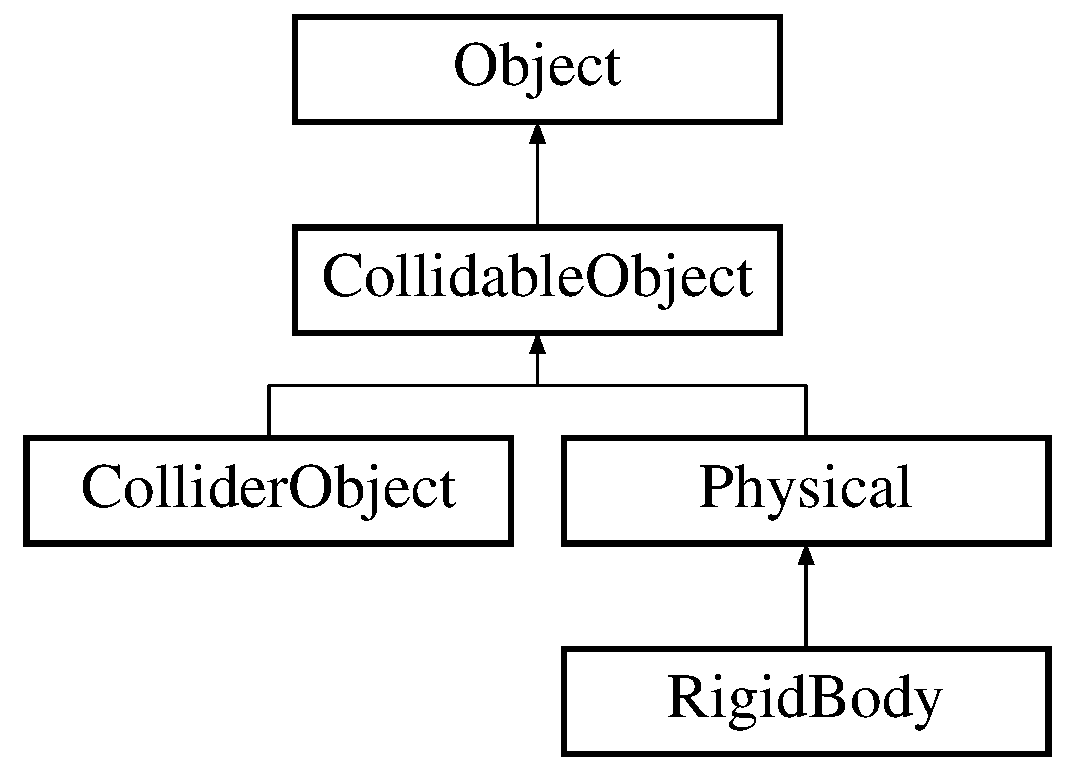
\includegraphics[height=4.000000cm]{class_collidable_object}
\end{center}
\end{figure}
\subsection*{Public Member Functions}
\begin{DoxyCompactItemize}
\item 
void \hyperlink{class_collidable_object_a3c8c31daabe129b6b7accb1759409a7b}{update} (const \hyperlink{class_p_b_time}{P\-B\-Time} \&\hyperlink{_physically_based_8h_a766da334af281a8fa1ed5cf404d0ec45}{the\-Time})
\item 
\hyperlink{class_collidable_object}{Collidable\-Object} $\ast$ \hyperlink{class_collidable_object_ab5a14a6929cecb22e3627f5e992bec36}{get\-Updated} (const \hyperlink{class_p_b_time}{P\-B\-Time} \&\hyperlink{_physically_based_8h_a766da334af281a8fa1ed5cf404d0ec45}{the\-Time})
\item 
virtual \hyperlink{class_deferred_force}{Deferred\-Force} $\ast$ \hyperlink{class_collidable_object_ad1ad2104aa96351a206ffe6540d84090}{get\-Collision\-Force} (const \hyperlink{class_collidable_object}{Collidable\-Object} \&updated, const \hyperlink{class_vector3_d}{Vector3\-D} \&normal)=0
\item 
bool \hyperlink{class_collidable_object_a3924392b72a5395d5327804d7700090d}{collision\-Check} (const \hyperlink{class_collidable_object}{Collidable\-Object} \&this\-Updated, const \hyperlink{class_collidable_object}{Collidable\-Object} \&other, const \hyperlink{class_collidable_object}{Collidable\-Object} \&other\-Updated, float \&timestep\-Frac, \hyperlink{class_collision_force}{Collision\-Force} \&collision\-Force)
\end{DoxyCompactItemize}
\subsection*{Protected Member Functions}
\begin{DoxyCompactItemize}
\item 
\hyperlink{class_collidable_object_a40008ad888dbfcf7b08a7850759b023e}{Collidable\-Object} ()
\item 
virtual void \hyperlink{class_collidable_object_a20734a532bf708d8fb5856483d5b8ed2}{update} (const \hyperlink{class_p_b_time}{P\-B\-Time} \&\hyperlink{_physically_based_8h_a766da334af281a8fa1ed5cf404d0ec45}{the\-Time}, \hyperlink{class_collidable_object}{Collidable\-Object} \&co)=0
\item 
virtual \hyperlink{class_collidable_object}{Collidable\-Object} $\ast$ \hyperlink{class_collidable_object_af7d1cf4164b033a6e68c5988d4b8aeb8}{clone} () const =0
\end{DoxyCompactItemize}
\subsection*{Protected Attributes}
\begin{DoxyCompactItemize}
\item 
\hyperlink{class_shape}{Shape} \& \hyperlink{class_collidable_object_afb18f5beeecf133e186219aecbde3b64}{collider}
\end{DoxyCompactItemize}
\subsection*{Additional Inherited Members}


\subsection{Constructor \& Destructor Documentation}
\hypertarget{class_collidable_object_a40008ad888dbfcf7b08a7850759b023e}{\index{Collidable\-Object@{Collidable\-Object}!Collidable\-Object@{Collidable\-Object}}
\index{Collidable\-Object@{Collidable\-Object}!CollidableObject@{Collidable\-Object}}
\subsubsection[{Collidable\-Object}]{\setlength{\rightskip}{0pt plus 5cm}Collidable\-Object\-::\-Collidable\-Object (
\begin{DoxyParamCaption}
{}
\end{DoxyParamCaption}
)\hspace{0.3cm}{\ttfamily [inline]}, {\ttfamily [protected]}}}\label{class_collidable_object_a40008ad888dbfcf7b08a7850759b023e}


\subsection{Member Function Documentation}
\hypertarget{class_collidable_object_af7d1cf4164b033a6e68c5988d4b8aeb8}{\index{Collidable\-Object@{Collidable\-Object}!clone@{clone}}
\index{clone@{clone}!CollidableObject@{Collidable\-Object}}
\subsubsection[{clone}]{\setlength{\rightskip}{0pt plus 5cm}virtual {\bf Collidable\-Object}$\ast$ Collidable\-Object\-::clone (
\begin{DoxyParamCaption}
{}
\end{DoxyParamCaption}
) const\hspace{0.3cm}{\ttfamily [protected]}, {\ttfamily [pure virtual]}}}\label{class_collidable_object_af7d1cf4164b033a6e68c5988d4b8aeb8}


Implemented in \hyperlink{class_collider_object_a5bdb3554ca95ddfe4045f17634537cca}{Collider\-Object}, and \hyperlink{class_physical_a8e6b99aec0d99df8e330881a25d936e6}{Physical}.

\hypertarget{class_collidable_object_a3924392b72a5395d5327804d7700090d}{\index{Collidable\-Object@{Collidable\-Object}!collision\-Check@{collision\-Check}}
\index{collision\-Check@{collision\-Check}!CollidableObject@{Collidable\-Object}}
\subsubsection[{collision\-Check}]{\setlength{\rightskip}{0pt plus 5cm}bool Collidable\-Object\-::collision\-Check (
\begin{DoxyParamCaption}
\item[{const {\bf Collidable\-Object} \&}]{this\-Updated, }
\item[{const {\bf Collidable\-Object} \&}]{other, }
\item[{const {\bf Collidable\-Object} \&}]{other\-Updated, }
\item[{float \&}]{timestep\-Frac, }
\item[{{\bf Collision\-Force} \&}]{collision\-Force}
\end{DoxyParamCaption}
)}}\label{class_collidable_object_a3924392b72a5395d5327804d7700090d}
\hypertarget{class_collidable_object_ad1ad2104aa96351a206ffe6540d84090}{\index{Collidable\-Object@{Collidable\-Object}!get\-Collision\-Force@{get\-Collision\-Force}}
\index{get\-Collision\-Force@{get\-Collision\-Force}!CollidableObject@{Collidable\-Object}}
\subsubsection[{get\-Collision\-Force}]{\setlength{\rightskip}{0pt plus 5cm}virtual {\bf Deferred\-Force}$\ast$ Collidable\-Object\-::get\-Collision\-Force (
\begin{DoxyParamCaption}
\item[{const {\bf Collidable\-Object} \&}]{updated, }
\item[{const {\bf Vector3\-D} \&}]{normal}
\end{DoxyParamCaption}
)\hspace{0.3cm}{\ttfamily [pure virtual]}}}\label{class_collidable_object_ad1ad2104aa96351a206ffe6540d84090}


Implemented in \hyperlink{class_rigid_body_a4b18eaaeb72f18c9f7d3f060d357e974}{Rigid\-Body}, and \hyperlink{class_collider_object_a9439b0a0d1465b07734f4886866c056f}{Collider\-Object}.

\hypertarget{class_collidable_object_ab5a14a6929cecb22e3627f5e992bec36}{\index{Collidable\-Object@{Collidable\-Object}!get\-Updated@{get\-Updated}}
\index{get\-Updated@{get\-Updated}!CollidableObject@{Collidable\-Object}}
\subsubsection[{get\-Updated}]{\setlength{\rightskip}{0pt plus 5cm}{\bf Collidable\-Object}$\ast$ Collidable\-Object\-::get\-Updated (
\begin{DoxyParamCaption}
\item[{const {\bf P\-B\-Time} \&}]{the\-Time}
\end{DoxyParamCaption}
)}}\label{class_collidable_object_ab5a14a6929cecb22e3627f5e992bec36}
\hypertarget{class_collidable_object_a3c8c31daabe129b6b7accb1759409a7b}{\index{Collidable\-Object@{Collidable\-Object}!update@{update}}
\index{update@{update}!CollidableObject@{Collidable\-Object}}
\subsubsection[{update}]{\setlength{\rightskip}{0pt plus 5cm}void Collidable\-Object\-::update (
\begin{DoxyParamCaption}
\item[{const {\bf P\-B\-Time} \&}]{the\-Time}
\end{DoxyParamCaption}
)}}\label{class_collidable_object_a3c8c31daabe129b6b7accb1759409a7b}
\hypertarget{class_collidable_object_a20734a532bf708d8fb5856483d5b8ed2}{\index{Collidable\-Object@{Collidable\-Object}!update@{update}}
\index{update@{update}!CollidableObject@{Collidable\-Object}}
\subsubsection[{update}]{\setlength{\rightskip}{0pt plus 5cm}virtual void Collidable\-Object\-::update (
\begin{DoxyParamCaption}
\item[{const {\bf P\-B\-Time} \&}]{the\-Time, }
\item[{{\bf Collidable\-Object} \&}]{co}
\end{DoxyParamCaption}
)\hspace{0.3cm}{\ttfamily [protected]}, {\ttfamily [pure virtual]}}}\label{class_collidable_object_a20734a532bf708d8fb5856483d5b8ed2}


Implemented in \hyperlink{class_collider_object_a3e8987fc6f558f65bb749f2144551483}{Collider\-Object}, and \hyperlink{class_physical_ac2f0c203798c646a9bffc9ef2bb64185}{Physical}.



\subsection{Member Data Documentation}
\hypertarget{class_collidable_object_afb18f5beeecf133e186219aecbde3b64}{\index{Collidable\-Object@{Collidable\-Object}!collider@{collider}}
\index{collider@{collider}!CollidableObject@{Collidable\-Object}}
\subsubsection[{collider}]{\setlength{\rightskip}{0pt plus 5cm}{\bf Shape}\& Collidable\-Object\-::collider\hspace{0.3cm}{\ttfamily [protected]}}}\label{class_collidable_object_afb18f5beeecf133e186219aecbde3b64}


The documentation for this class was generated from the following file\-:\begin{DoxyCompactItemize}
\item 
D\-:/\-Development/\-My\-Projects/\-Physically\-Based\-Modeling/include/\hyperlink{_collidable_object_8h}{Collidable\-Object.\-h}\end{DoxyCompactItemize}

\hypertarget{class_collider_object}{\section{Collider\-Object Class Reference}
\label{class_collider_object}\index{Collider\-Object@{Collider\-Object}}
}


{\ttfamily \#include $<$Collider\-Object.\-h$>$}

Inheritance diagram for Collider\-Object\-:\begin{figure}[H]
\begin{center}
\leavevmode
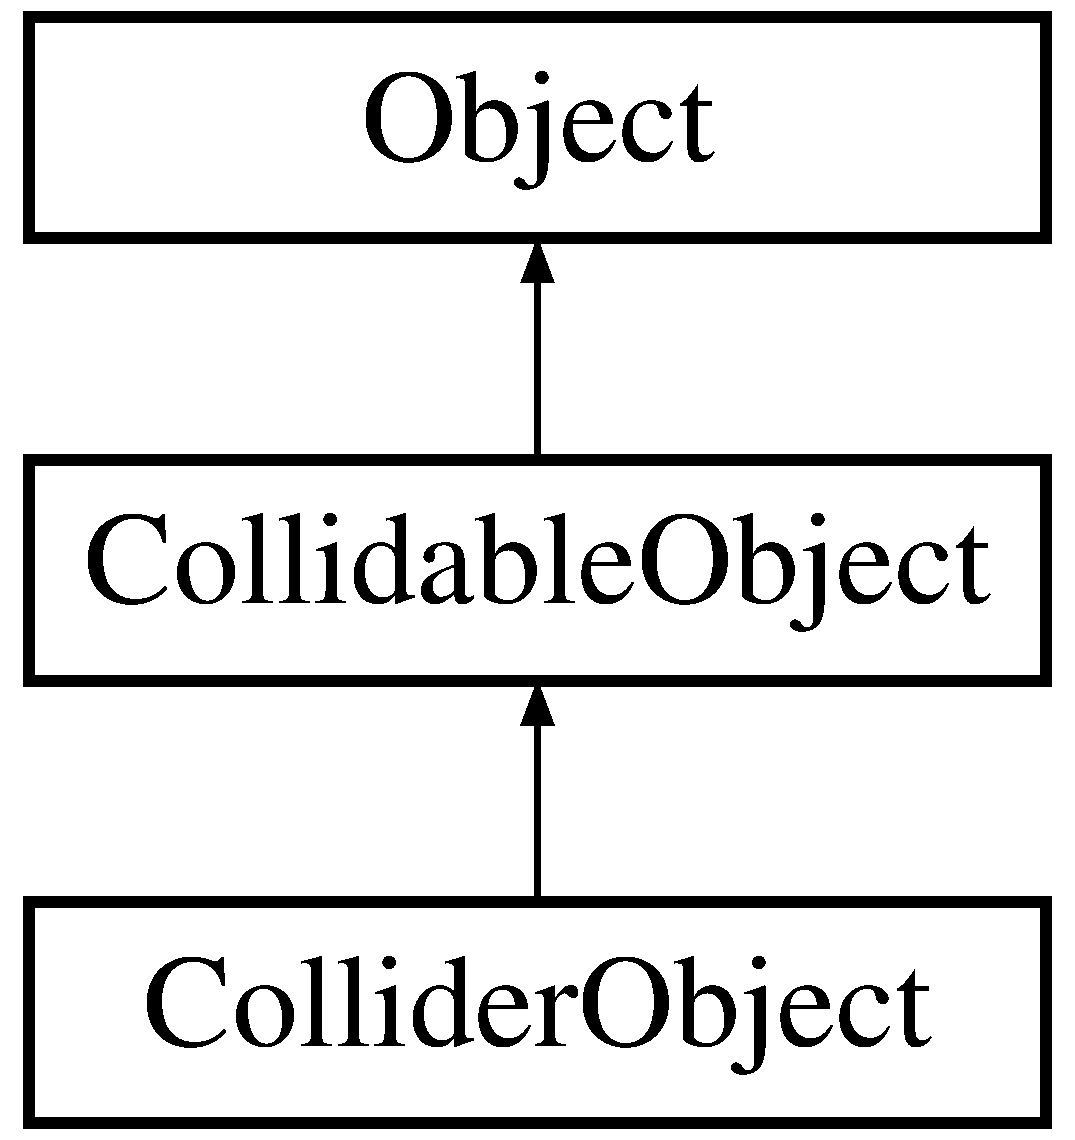
\includegraphics[height=3.000000cm]{class_collider_object}
\end{center}
\end{figure}
\subsection*{Public Member Functions}
\begin{DoxyCompactItemize}
\item 
\hyperlink{class_collider_object_a08f4c5989ad7601eb05837179cf17aac}{Collider\-Object} ()
\item 
virtual \hyperlink{class_deferred_force}{Deferred\-Force} $\ast$ \hyperlink{class_collider_object_a9439b0a0d1465b07734f4886866c056f}{get\-Collision\-Force} (const \hyperlink{class_collidable_object}{Collidable\-Object} \&co, const \hyperlink{class_vector3_d}{Vector3\-D} \&normal)
\end{DoxyCompactItemize}
\subsection*{Protected Member Functions}
\begin{DoxyCompactItemize}
\item 
virtual void \hyperlink{class_collider_object_a3e8987fc6f558f65bb749f2144551483}{update} (const \hyperlink{class_p_b_time}{P\-B\-Time} \&\hyperlink{_physically_based_8h_a766da334af281a8fa1ed5cf404d0ec45}{the\-Time}, \hyperlink{class_collidable_object}{Collidable\-Object} \&co)
\item 
virtual \hyperlink{class_collider_object}{Collider\-Object} $\ast$ \hyperlink{class_collider_object_a5bdb3554ca95ddfe4045f17634537cca}{clone} () const 
\end{DoxyCompactItemize}
\subsection*{Additional Inherited Members}


\subsection{Constructor \& Destructor Documentation}
\hypertarget{class_collider_object_a08f4c5989ad7601eb05837179cf17aac}{\index{Collider\-Object@{Collider\-Object}!Collider\-Object@{Collider\-Object}}
\index{Collider\-Object@{Collider\-Object}!ColliderObject@{Collider\-Object}}
\subsubsection[{Collider\-Object}]{\setlength{\rightskip}{0pt plus 5cm}Collider\-Object\-::\-Collider\-Object (
\begin{DoxyParamCaption}
{}
\end{DoxyParamCaption}
)\hspace{0.3cm}{\ttfamily [inline]}}}\label{class_collider_object_a08f4c5989ad7601eb05837179cf17aac}


\subsection{Member Function Documentation}
\hypertarget{class_collider_object_a5bdb3554ca95ddfe4045f17634537cca}{\index{Collider\-Object@{Collider\-Object}!clone@{clone}}
\index{clone@{clone}!ColliderObject@{Collider\-Object}}
\subsubsection[{clone}]{\setlength{\rightskip}{0pt plus 5cm}virtual {\bf Collider\-Object}$\ast$ Collider\-Object\-::clone (
\begin{DoxyParamCaption}
{}
\end{DoxyParamCaption}
) const\hspace{0.3cm}{\ttfamily [inline]}, {\ttfamily [protected]}, {\ttfamily [virtual]}}}\label{class_collider_object_a5bdb3554ca95ddfe4045f17634537cca}


Implements \hyperlink{class_collidable_object_af7d1cf4164b033a6e68c5988d4b8aeb8}{Collidable\-Object}.

\hypertarget{class_collider_object_a9439b0a0d1465b07734f4886866c056f}{\index{Collider\-Object@{Collider\-Object}!get\-Collision\-Force@{get\-Collision\-Force}}
\index{get\-Collision\-Force@{get\-Collision\-Force}!ColliderObject@{Collider\-Object}}
\subsubsection[{get\-Collision\-Force}]{\setlength{\rightskip}{0pt plus 5cm}virtual {\bf Deferred\-Force}$\ast$ Collider\-Object\-::get\-Collision\-Force (
\begin{DoxyParamCaption}
\item[{const {\bf Collidable\-Object} \&}]{co, }
\item[{const {\bf Vector3\-D} \&}]{normal}
\end{DoxyParamCaption}
)\hspace{0.3cm}{\ttfamily [inline]}, {\ttfamily [virtual]}}}\label{class_collider_object_a9439b0a0d1465b07734f4886866c056f}


Implements \hyperlink{class_collidable_object_ad1ad2104aa96351a206ffe6540d84090}{Collidable\-Object}.

\hypertarget{class_collider_object_a3e8987fc6f558f65bb749f2144551483}{\index{Collider\-Object@{Collider\-Object}!update@{update}}
\index{update@{update}!ColliderObject@{Collider\-Object}}
\subsubsection[{update}]{\setlength{\rightskip}{0pt plus 5cm}virtual void Collider\-Object\-::update (
\begin{DoxyParamCaption}
\item[{const {\bf P\-B\-Time} \&}]{the\-Time, }
\item[{{\bf Collidable\-Object} \&}]{co}
\end{DoxyParamCaption}
)\hspace{0.3cm}{\ttfamily [inline]}, {\ttfamily [protected]}, {\ttfamily [virtual]}}}\label{class_collider_object_a3e8987fc6f558f65bb749f2144551483}


Implements \hyperlink{class_collidable_object_a20734a532bf708d8fb5856483d5b8ed2}{Collidable\-Object}.



The documentation for this class was generated from the following file\-:\begin{DoxyCompactItemize}
\item 
D\-:/\-Development/\-My\-Projects/\-Physically\-Based\-Modeling/include/\hyperlink{_collider_object_8h}{Collider\-Object.\-h}\end{DoxyCompactItemize}

\hypertarget{class_collision_force}{\section{Collision\-Force Class Reference}
\label{class_collision_force}\index{Collision\-Force@{Collision\-Force}}
}


{\ttfamily \#include $<$Collidable\-Object.\-h$>$}

\subsection*{Public Member Functions}
\begin{DoxyCompactItemize}
\item 
\hyperlink{class_collision_force_a3781a639cf9229971db982facaa16e4f}{Collision\-Force} ()
\item 
virtual void \hyperlink{class_collision_force_a94c4bb70d3d19b58aab28ca717614582}{$\sim$\-Collision\-Force} ()
\item 
\hyperlink{class_independent_force}{Independent\-Force} \hyperlink{class_collision_force_a21e2c74bc0e6be829df48d1b036d20c6}{get} (const \hyperlink{class_p_b_time}{P\-B\-Time} \&\hyperlink{_physically_based_8h_a766da334af281a8fa1ed5cf404d0ec45}{the\-Time}) const 
\item 
void \hyperlink{class_collision_force_af4381b3c21af2d0c34042c55b211e061}{set} (\hyperlink{class_deferred_force}{Deferred\-Force} $\ast$a, \hyperlink{class_deferred_force}{Deferred\-Force} $\ast$b)
\end{DoxyCompactItemize}


\subsection{Constructor \& Destructor Documentation}
\hypertarget{class_collision_force_a3781a639cf9229971db982facaa16e4f}{\index{Collision\-Force@{Collision\-Force}!Collision\-Force@{Collision\-Force}}
\index{Collision\-Force@{Collision\-Force}!CollisionForce@{Collision\-Force}}
\subsubsection[{Collision\-Force}]{\setlength{\rightskip}{0pt plus 5cm}Collision\-Force\-::\-Collision\-Force (
\begin{DoxyParamCaption}
{}
\end{DoxyParamCaption}
)\hspace{0.3cm}{\ttfamily [inline]}}}\label{class_collision_force_a3781a639cf9229971db982facaa16e4f}
\hypertarget{class_collision_force_a94c4bb70d3d19b58aab28ca717614582}{\index{Collision\-Force@{Collision\-Force}!$\sim$\-Collision\-Force@{$\sim$\-Collision\-Force}}
\index{$\sim$\-Collision\-Force@{$\sim$\-Collision\-Force}!CollisionForce@{Collision\-Force}}
\subsubsection[{$\sim$\-Collision\-Force}]{\setlength{\rightskip}{0pt plus 5cm}virtual void Collision\-Force\-::$\sim$\-Collision\-Force (
\begin{DoxyParamCaption}
{}
\end{DoxyParamCaption}
)\hspace{0.3cm}{\ttfamily [inline]}, {\ttfamily [virtual]}}}\label{class_collision_force_a94c4bb70d3d19b58aab28ca717614582}


\subsection{Member Function Documentation}
\hypertarget{class_collision_force_a21e2c74bc0e6be829df48d1b036d20c6}{\index{Collision\-Force@{Collision\-Force}!get@{get}}
\index{get@{get}!CollisionForce@{Collision\-Force}}
\subsubsection[{get}]{\setlength{\rightskip}{0pt plus 5cm}{\bf Independent\-Force} Collision\-Force\-::get (
\begin{DoxyParamCaption}
\item[{const {\bf P\-B\-Time} \&}]{the\-Time}
\end{DoxyParamCaption}
) const\hspace{0.3cm}{\ttfamily [inline]}}}\label{class_collision_force_a21e2c74bc0e6be829df48d1b036d20c6}
\hypertarget{class_collision_force_af4381b3c21af2d0c34042c55b211e061}{\index{Collision\-Force@{Collision\-Force}!set@{set}}
\index{set@{set}!CollisionForce@{Collision\-Force}}
\subsubsection[{set}]{\setlength{\rightskip}{0pt plus 5cm}void Collision\-Force\-::set (
\begin{DoxyParamCaption}
\item[{{\bf Deferred\-Force} $\ast$}]{a, }
\item[{{\bf Deferred\-Force} $\ast$}]{b}
\end{DoxyParamCaption}
)\hspace{0.3cm}{\ttfamily [inline]}}}\label{class_collision_force_af4381b3c21af2d0c34042c55b211e061}


The documentation for this class was generated from the following file\-:\begin{DoxyCompactItemize}
\item 
D\-:/\-Development/\-My\-Projects/\-Physically\-Based\-Modeling/include/\hyperlink{_collidable_object_8h}{Collidable\-Object.\-h}\end{DoxyCompactItemize}

\hypertarget{class_deferred_force}{\section{Deferred\-Force Class Reference}
\label{class_deferred_force}\index{Deferred\-Force@{Deferred\-Force}}
}


{\ttfamily \#include $<$Collidable\-Object.\-h$>$}

Inheritance diagram for Deferred\-Force\-:\begin{figure}[H]
\begin{center}
\leavevmode
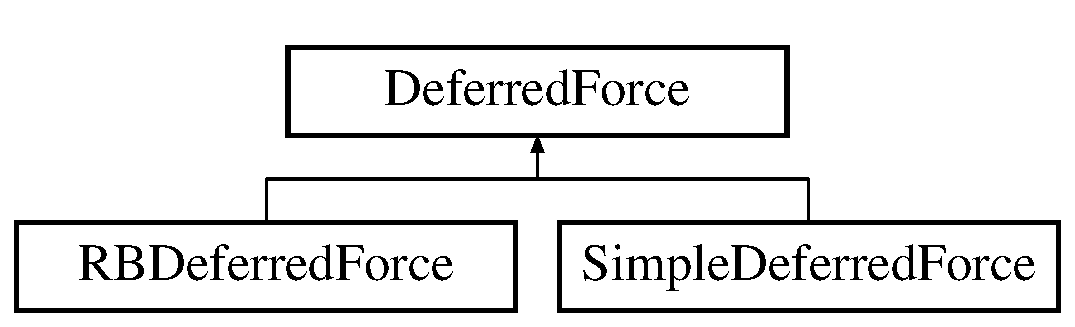
\includegraphics[height=2.000000cm]{class_deferred_force}
\end{center}
\end{figure}
\subsection*{Public Member Functions}
\begin{DoxyCompactItemize}
\item 
virtual \hyperlink{class_force}{Force} $\ast$ \hyperlink{class_deferred_force_adb04f317b659e80b803b54c5890dc170}{get} (float \hyperlink{_physically_based_8h_ab9edcc09985767509bf717e25ac80ab7}{timestep}) const =0
\end{DoxyCompactItemize}
\subsection*{Protected Member Functions}
\begin{DoxyCompactItemize}
\item 
\hyperlink{class_deferred_force_abea6ed39987141076ee24270c920cbe5}{Deferred\-Force} ()
\end{DoxyCompactItemize}


\subsection{Constructor \& Destructor Documentation}
\hypertarget{class_deferred_force_abea6ed39987141076ee24270c920cbe5}{\index{Deferred\-Force@{Deferred\-Force}!Deferred\-Force@{Deferred\-Force}}
\index{Deferred\-Force@{Deferred\-Force}!DeferredForce@{Deferred\-Force}}
\subsubsection[{Deferred\-Force}]{\setlength{\rightskip}{0pt plus 5cm}Deferred\-Force\-::\-Deferred\-Force (
\begin{DoxyParamCaption}
{}
\end{DoxyParamCaption}
)\hspace{0.3cm}{\ttfamily [inline]}, {\ttfamily [protected]}}}\label{class_deferred_force_abea6ed39987141076ee24270c920cbe5}


\subsection{Member Function Documentation}
\hypertarget{class_deferred_force_adb04f317b659e80b803b54c5890dc170}{\index{Deferred\-Force@{Deferred\-Force}!get@{get}}
\index{get@{get}!DeferredForce@{Deferred\-Force}}
\subsubsection[{get}]{\setlength{\rightskip}{0pt plus 5cm}virtual {\bf Force}$\ast$ Deferred\-Force\-::get (
\begin{DoxyParamCaption}
\item[{float}]{timestep}
\end{DoxyParamCaption}
) const\hspace{0.3cm}{\ttfamily [pure virtual]}}}\label{class_deferred_force_adb04f317b659e80b803b54c5890dc170}


The documentation for this class was generated from the following file\-:\begin{DoxyCompactItemize}
\item 
D\-:/\-Development/\-My\-Projects/\-Physically\-Based\-Modeling/include/\hyperlink{_collidable_object_8h}{Collidable\-Object.\-h}\end{DoxyCompactItemize}

\hypertarget{class_environment}{\section{Environment Class Reference}
\label{class_environment}\index{Environment@{Environment}}
}


{\ttfamily \#include $<$Environment.\-h$>$}

\subsection*{Public Member Functions}
\begin{DoxyCompactItemize}
\item 
\hyperlink{class_environment_a8b427c4448d8b7536666837521b9e83d}{Environment} ()
\item 
\hyperlink{class_environment_a23d58e47f81b141b2802e3f0b730c154}{Environment} (const \hyperlink{class_transform}{Transform} \&t)
\item 
void \hyperlink{class_environment_ad32cd563f0849fcbb097c5b05c6646ed}{add\-Force\-Environment} (const \hyperlink{class_force_environment}{Force\-Environment} \&fe)
\item 
void \hyperlink{class_environment_ac09236d36211cdbf2836aca73847cd8c}{add\-Collidable} (const \hyperlink{class_collidable_object}{Collidable\-Object} \&co)
\item 
void \hyperlink{class_environment_a33f09db8b861a0eb48ea0310560180d8}{add\-Physical} (const \hyperlink{class_physical}{Physical} \&ph)
\item 
void \hyperlink{class_environment_a58ed629cb5f416d9b311dbb3f8f776c4}{link\-Force\-Env} (unsigned int physical, unsigned int force\-Env)
\item 
void \hyperlink{class_environment_ad969e09a5ccb33b3948f35b80649f279}{update} (const \hyperlink{class_p_b_time}{P\-B\-Time} \&\hyperlink{_physically_based_8h_a766da334af281a8fa1ed5cf404d0ec45}{the\-Time})
\end{DoxyCompactItemize}
\subsection*{Public Attributes}
\begin{DoxyCompactItemize}
\item 
\hyperlink{class_transform}{Transform} \hyperlink{class_environment_a334e187e5b58de5e60161627e9196ee3}{transform}
\end{DoxyCompactItemize}


\subsection{Constructor \& Destructor Documentation}
\hypertarget{class_environment_a8b427c4448d8b7536666837521b9e83d}{\index{Environment@{Environment}!Environment@{Environment}}
\index{Environment@{Environment}!Environment@{Environment}}
\subsubsection[{Environment}]{\setlength{\rightskip}{0pt plus 5cm}Environment\-::\-Environment (
\begin{DoxyParamCaption}
{}
\end{DoxyParamCaption}
)}}\label{class_environment_a8b427c4448d8b7536666837521b9e83d}
\hypertarget{class_environment_a23d58e47f81b141b2802e3f0b730c154}{\index{Environment@{Environment}!Environment@{Environment}}
\index{Environment@{Environment}!Environment@{Environment}}
\subsubsection[{Environment}]{\setlength{\rightskip}{0pt plus 5cm}Environment\-::\-Environment (
\begin{DoxyParamCaption}
\item[{const {\bf Transform} \&}]{t}
\end{DoxyParamCaption}
)}}\label{class_environment_a23d58e47f81b141b2802e3f0b730c154}


\subsection{Member Function Documentation}
\hypertarget{class_environment_ac09236d36211cdbf2836aca73847cd8c}{\index{Environment@{Environment}!add\-Collidable@{add\-Collidable}}
\index{add\-Collidable@{add\-Collidable}!Environment@{Environment}}
\subsubsection[{add\-Collidable}]{\setlength{\rightskip}{0pt plus 5cm}void Environment\-::add\-Collidable (
\begin{DoxyParamCaption}
\item[{const {\bf Collidable\-Object} \&}]{co}
\end{DoxyParamCaption}
)}}\label{class_environment_ac09236d36211cdbf2836aca73847cd8c}
\hypertarget{class_environment_ad32cd563f0849fcbb097c5b05c6646ed}{\index{Environment@{Environment}!add\-Force\-Environment@{add\-Force\-Environment}}
\index{add\-Force\-Environment@{add\-Force\-Environment}!Environment@{Environment}}
\subsubsection[{add\-Force\-Environment}]{\setlength{\rightskip}{0pt plus 5cm}void Environment\-::add\-Force\-Environment (
\begin{DoxyParamCaption}
\item[{const {\bf Force\-Environment} \&}]{fe}
\end{DoxyParamCaption}
)}}\label{class_environment_ad32cd563f0849fcbb097c5b05c6646ed}
\hypertarget{class_environment_a33f09db8b861a0eb48ea0310560180d8}{\index{Environment@{Environment}!add\-Physical@{add\-Physical}}
\index{add\-Physical@{add\-Physical}!Environment@{Environment}}
\subsubsection[{add\-Physical}]{\setlength{\rightskip}{0pt plus 5cm}void Environment\-::add\-Physical (
\begin{DoxyParamCaption}
\item[{const {\bf Physical} \&}]{ph}
\end{DoxyParamCaption}
)}}\label{class_environment_a33f09db8b861a0eb48ea0310560180d8}
\hypertarget{class_environment_a58ed629cb5f416d9b311dbb3f8f776c4}{\index{Environment@{Environment}!link\-Force\-Env@{link\-Force\-Env}}
\index{link\-Force\-Env@{link\-Force\-Env}!Environment@{Environment}}
\subsubsection[{link\-Force\-Env}]{\setlength{\rightskip}{0pt plus 5cm}void Environment\-::link\-Force\-Env (
\begin{DoxyParamCaption}
\item[{unsigned int}]{physical, }
\item[{unsigned int}]{force\-Env}
\end{DoxyParamCaption}
)}}\label{class_environment_a58ed629cb5f416d9b311dbb3f8f776c4}
\hypertarget{class_environment_ad969e09a5ccb33b3948f35b80649f279}{\index{Environment@{Environment}!update@{update}}
\index{update@{update}!Environment@{Environment}}
\subsubsection[{update}]{\setlength{\rightskip}{0pt plus 5cm}void Environment\-::update (
\begin{DoxyParamCaption}
\item[{const {\bf P\-B\-Time} \&}]{the\-Time}
\end{DoxyParamCaption}
)}}\label{class_environment_ad969e09a5ccb33b3948f35b80649f279}


\subsection{Member Data Documentation}
\hypertarget{class_environment_a334e187e5b58de5e60161627e9196ee3}{\index{Environment@{Environment}!transform@{transform}}
\index{transform@{transform}!Environment@{Environment}}
\subsubsection[{transform}]{\setlength{\rightskip}{0pt plus 5cm}{\bf Transform} Environment\-::transform}}\label{class_environment_a334e187e5b58de5e60161627e9196ee3}


The documentation for this class was generated from the following file\-:\begin{DoxyCompactItemize}
\item 
D\-:/\-Development/\-My\-Projects/\-Physically\-Based\-Modeling/include/\hyperlink{_environment_8h}{Environment.\-h}\end{DoxyCompactItemize}

\hypertarget{class_force}{\section{Force Class Reference}
\label{class_force}\index{Force@{Force}}
}


{\ttfamily \#include $<$Force.\-h$>$}

Inheritance diagram for Force\-:\begin{figure}[H]
\begin{center}
\leavevmode
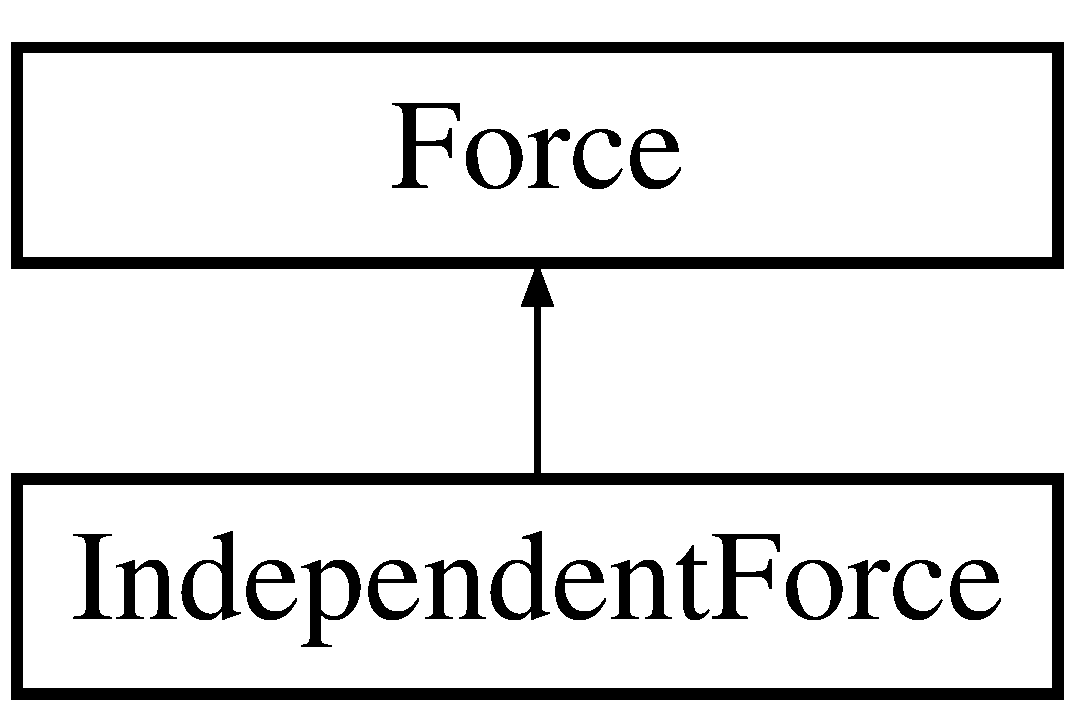
\includegraphics[height=2.000000cm]{class_force}
\end{center}
\end{figure}
\subsection*{Public Member Functions}
\begin{DoxyCompactItemize}
\item 
virtual \hyperlink{class_vector3_d}{Vector3\-D} \hyperlink{class_force_afa6cdb1fe5f0d009e72fafa663147744}{get} (float time) const =0
\end{DoxyCompactItemize}
\subsection*{Protected Member Functions}
\begin{DoxyCompactItemize}
\item 
\hyperlink{class_force_a00983e3bbc206a00bb9253deafc4e424}{Force} ()
\end{DoxyCompactItemize}


\subsection{Constructor \& Destructor Documentation}
\hypertarget{class_force_a00983e3bbc206a00bb9253deafc4e424}{\index{Force@{Force}!Force@{Force}}
\index{Force@{Force}!Force@{Force}}
\subsubsection[{Force}]{\setlength{\rightskip}{0pt plus 5cm}Force\-::\-Force (
\begin{DoxyParamCaption}
{}
\end{DoxyParamCaption}
)\hspace{0.3cm}{\ttfamily [inline]}, {\ttfamily [protected]}}}\label{class_force_a00983e3bbc206a00bb9253deafc4e424}


\subsection{Member Function Documentation}
\hypertarget{class_force_afa6cdb1fe5f0d009e72fafa663147744}{\index{Force@{Force}!get@{get}}
\index{get@{get}!Force@{Force}}
\subsubsection[{get}]{\setlength{\rightskip}{0pt plus 5cm}virtual {\bf Vector3\-D} Force\-::get (
\begin{DoxyParamCaption}
\item[{float}]{time}
\end{DoxyParamCaption}
) const\hspace{0.3cm}{\ttfamily [pure virtual]}}}\label{class_force_afa6cdb1fe5f0d009e72fafa663147744}


Implemented in \hyperlink{class_independent_force_aeb5118d339cbe545db0bfbf47c4b5b68}{Independent\-Force}.



The documentation for this class was generated from the following file\-:\begin{DoxyCompactItemize}
\item 
D\-:/\-Development/\-My\-Projects/\-Physically\-Based\-Modeling/include/\hyperlink{_force_8h}{Force.\-h}\end{DoxyCompactItemize}

\hypertarget{class_force_environment}{\section{Force\-Environment Class Reference}
\label{class_force_environment}\index{Force\-Environment@{Force\-Environment}}
}


{\ttfamily \#include $<$Force\-Environment.\-h$>$}

\subsection*{Public Types}
\begin{DoxyCompactItemize}
\item 
enum \hyperlink{class_force_environment_afe538e13c2d311649eb40395b05e6838}{force\-Type} \{ \hyperlink{class_force_environment_afe538e13c2d311649eb40395b05e6838abb0afa714bfff1d26b3ea9fcbb92ec26}{F\-O\-R\-C\-E}, 
\hyperlink{class_force_environment_afe538e13c2d311649eb40395b05e6838a5298601d31daac5af1b571bb22a2565c}{A\-C\-C\-E\-L\-E\-R\-A\-T\-I\-O\-N}
 \}
\end{DoxyCompactItemize}
\subsection*{Public Member Functions}
\begin{DoxyCompactItemize}
\item 
\hyperlink{class_force_environment_add872e8e7c7cf4b237d793422ed2383e}{Force\-Environment} ()
\item 
void \hyperlink{class_force_environment_a68a551c582e2b96f08b86907120e2df8}{add\-Force} (const \hyperlink{class_force}{Force} \&f, \hyperlink{class_force_environment_afe538e13c2d311649eb40395b05e6838}{force\-Type} t)
\end{DoxyCompactItemize}
\subsection*{Friends}
\begin{DoxyCompactItemize}
\item 
class \hyperlink{class_force_environment_ad07f4de926e4e68b49b17ab4d13369d3}{Environment}
\end{DoxyCompactItemize}


\subsection{Member Enumeration Documentation}
\hypertarget{class_force_environment_afe538e13c2d311649eb40395b05e6838}{\index{Force\-Environment@{Force\-Environment}!force\-Type@{force\-Type}}
\index{force\-Type@{force\-Type}!ForceEnvironment@{Force\-Environment}}
\subsubsection[{force\-Type}]{\setlength{\rightskip}{0pt plus 5cm}enum {\bf Force\-Environment\-::force\-Type}}}\label{class_force_environment_afe538e13c2d311649eb40395b05e6838}
\begin{Desc}
\item[Enumerator]\par
\begin{description}
\index{F\-O\-R\-C\-E@{F\-O\-R\-C\-E}!Force\-Environment@{Force\-Environment}}\index{Force\-Environment@{Force\-Environment}!F\-O\-R\-C\-E@{F\-O\-R\-C\-E}}\item[{\em 
\hypertarget{class_force_environment_afe538e13c2d311649eb40395b05e6838abb0afa714bfff1d26b3ea9fcbb92ec26}{F\-O\-R\-C\-E}\label{class_force_environment_afe538e13c2d311649eb40395b05e6838abb0afa714bfff1d26b3ea9fcbb92ec26}
}]\index{A\-C\-C\-E\-L\-E\-R\-A\-T\-I\-O\-N@{A\-C\-C\-E\-L\-E\-R\-A\-T\-I\-O\-N}!Force\-Environment@{Force\-Environment}}\index{Force\-Environment@{Force\-Environment}!A\-C\-C\-E\-L\-E\-R\-A\-T\-I\-O\-N@{A\-C\-C\-E\-L\-E\-R\-A\-T\-I\-O\-N}}\item[{\em 
\hypertarget{class_force_environment_afe538e13c2d311649eb40395b05e6838a5298601d31daac5af1b571bb22a2565c}{A\-C\-C\-E\-L\-E\-R\-A\-T\-I\-O\-N}\label{class_force_environment_afe538e13c2d311649eb40395b05e6838a5298601d31daac5af1b571bb22a2565c}
}]\end{description}
\end{Desc}


\subsection{Constructor \& Destructor Documentation}
\hypertarget{class_force_environment_add872e8e7c7cf4b237d793422ed2383e}{\index{Force\-Environment@{Force\-Environment}!Force\-Environment@{Force\-Environment}}
\index{Force\-Environment@{Force\-Environment}!ForceEnvironment@{Force\-Environment}}
\subsubsection[{Force\-Environment}]{\setlength{\rightskip}{0pt plus 5cm}Force\-Environment\-::\-Force\-Environment (
\begin{DoxyParamCaption}
{}
\end{DoxyParamCaption}
)}}\label{class_force_environment_add872e8e7c7cf4b237d793422ed2383e}


\subsection{Member Function Documentation}
\hypertarget{class_force_environment_a68a551c582e2b96f08b86907120e2df8}{\index{Force\-Environment@{Force\-Environment}!add\-Force@{add\-Force}}
\index{add\-Force@{add\-Force}!ForceEnvironment@{Force\-Environment}}
\subsubsection[{add\-Force}]{\setlength{\rightskip}{0pt plus 5cm}void Force\-Environment\-::add\-Force (
\begin{DoxyParamCaption}
\item[{const {\bf Force} \&}]{f, }
\item[{{\bf force\-Type}}]{t}
\end{DoxyParamCaption}
)\hspace{0.3cm}{\ttfamily [inline]}}}\label{class_force_environment_a68a551c582e2b96f08b86907120e2df8}


\subsection{Friends And Related Function Documentation}
\hypertarget{class_force_environment_ad07f4de926e4e68b49b17ab4d13369d3}{\index{Force\-Environment@{Force\-Environment}!Environment@{Environment}}
\index{Environment@{Environment}!ForceEnvironment@{Force\-Environment}}
\subsubsection[{Environment}]{\setlength{\rightskip}{0pt plus 5cm}friend class {\bf Environment}\hspace{0.3cm}{\ttfamily [friend]}}}\label{class_force_environment_ad07f4de926e4e68b49b17ab4d13369d3}


The documentation for this class was generated from the following file\-:\begin{DoxyCompactItemize}
\item 
D\-:/\-Development/\-My\-Projects/\-Physically\-Based\-Modeling/include/\hyperlink{_force_environment_8h}{Force\-Environment.\-h}\end{DoxyCompactItemize}

\hypertarget{class_hi_def_color}{\section{Hi\-Def\-Color Class Reference}
\label{class_hi_def_color}\index{Hi\-Def\-Color@{Hi\-Def\-Color}}
}


{\ttfamily \#include $<$Utility.\-h$>$}

\subsection*{Public Member Functions}
\begin{DoxyCompactItemize}
\item 
\hyperlink{class_hi_def_color_a36ec3082115008dfa06a3f5e76b679cf}{Hi\-Def\-Color} ()
\item 
\hyperlink{class_hi_def_color_a488b3cda33c527688e860e23719ad14b}{Hi\-Def\-Color} (float \hyperlink{class_hi_def_color_ab04783d755f14245ce7482aa68e5bbd7}{r}, float \hyperlink{class_hi_def_color_a63606164cca043b989cc904f6dfd1b12}{g}, float \hyperlink{class_hi_def_color_a783305313073eed854522db82459c185}{b})
\item 
\hyperlink{class_hi_def_color_a50b7fe57efaf975deaccba71057b4dee}{Hi\-Def\-Color} (const \hyperlink{class_hi_def_color}{Hi\-Def\-Color} \&clr)
\item 
\hyperlink{class_hi_def_color}{Hi\-Def\-Color} \& \hyperlink{class_hi_def_color_aa4c1ef6d9e3338962f8e68d3086ecde0}{operator=} (const \hyperlink{class_hi_def_color}{Hi\-Def\-Color} \&rhs)
\item 
\hyperlink{class_hi_def_color}{Hi\-Def\-Color} \& \hyperlink{class_hi_def_color_a80daa3de1eb6c526074a0401509aae12}{operator+=} (const \hyperlink{class_hi_def_color}{Hi\-Def\-Color} \&rhs)
\end{DoxyCompactItemize}
\subsection*{Public Attributes}
\begin{DoxyCompactItemize}
\item 
float \hyperlink{class_hi_def_color_ab04783d755f14245ce7482aa68e5bbd7}{r}
\item 
float \hyperlink{class_hi_def_color_a63606164cca043b989cc904f6dfd1b12}{g}
\item 
float \hyperlink{class_hi_def_color_a783305313073eed854522db82459c185}{b}
\end{DoxyCompactItemize}
\subsection*{Friends}
\begin{DoxyCompactItemize}
\item 
\hyperlink{class_hi_def_color}{Hi\-Def\-Color} \hyperlink{class_hi_def_color_acb6d7c39f2e4766080ba115fd16807f3}{operator+} (const \hyperlink{class_hi_def_color}{Hi\-Def\-Color} \&c1, const \hyperlink{class_hi_def_color}{Hi\-Def\-Color} \&c2)
\item 
\hyperlink{class_hi_def_color}{Hi\-Def\-Color} \hyperlink{class_hi_def_color_af03c6dfd98fdb24c983d536686bcc065}{operator-\/} (const \hyperlink{class_hi_def_color}{Hi\-Def\-Color} \&c1, const \hyperlink{class_hi_def_color}{Hi\-Def\-Color} \&c2)
\item 
\hyperlink{class_hi_def_color}{Hi\-Def\-Color} \hyperlink{class_hi_def_color_adce5dfbc8cc2a59c44996cc050a2609e}{operator$\ast$} (const \hyperlink{class_hi_def_color}{Hi\-Def\-Color} \&lhs, double rhs)
\end{DoxyCompactItemize}


\subsection{Constructor \& Destructor Documentation}
\hypertarget{class_hi_def_color_a36ec3082115008dfa06a3f5e76b679cf}{\index{Hi\-Def\-Color@{Hi\-Def\-Color}!Hi\-Def\-Color@{Hi\-Def\-Color}}
\index{Hi\-Def\-Color@{Hi\-Def\-Color}!HiDefColor@{Hi\-Def\-Color}}
\subsubsection[{Hi\-Def\-Color}]{\setlength{\rightskip}{0pt plus 5cm}Hi\-Def\-Color\-::\-Hi\-Def\-Color (
\begin{DoxyParamCaption}
{}
\end{DoxyParamCaption}
)\hspace{0.3cm}{\ttfamily [inline]}}}\label{class_hi_def_color_a36ec3082115008dfa06a3f5e76b679cf}
\hypertarget{class_hi_def_color_a488b3cda33c527688e860e23719ad14b}{\index{Hi\-Def\-Color@{Hi\-Def\-Color}!Hi\-Def\-Color@{Hi\-Def\-Color}}
\index{Hi\-Def\-Color@{Hi\-Def\-Color}!HiDefColor@{Hi\-Def\-Color}}
\subsubsection[{Hi\-Def\-Color}]{\setlength{\rightskip}{0pt plus 5cm}Hi\-Def\-Color\-::\-Hi\-Def\-Color (
\begin{DoxyParamCaption}
\item[{float}]{r, }
\item[{float}]{g, }
\item[{float}]{b}
\end{DoxyParamCaption}
)\hspace{0.3cm}{\ttfamily [inline]}}}\label{class_hi_def_color_a488b3cda33c527688e860e23719ad14b}
\hypertarget{class_hi_def_color_a50b7fe57efaf975deaccba71057b4dee}{\index{Hi\-Def\-Color@{Hi\-Def\-Color}!Hi\-Def\-Color@{Hi\-Def\-Color}}
\index{Hi\-Def\-Color@{Hi\-Def\-Color}!HiDefColor@{Hi\-Def\-Color}}
\subsubsection[{Hi\-Def\-Color}]{\setlength{\rightskip}{0pt plus 5cm}Hi\-Def\-Color\-::\-Hi\-Def\-Color (
\begin{DoxyParamCaption}
\item[{const {\bf Hi\-Def\-Color} \&}]{clr}
\end{DoxyParamCaption}
)\hspace{0.3cm}{\ttfamily [inline]}}}\label{class_hi_def_color_a50b7fe57efaf975deaccba71057b4dee}


\subsection{Member Function Documentation}
\hypertarget{class_hi_def_color_a80daa3de1eb6c526074a0401509aae12}{\index{Hi\-Def\-Color@{Hi\-Def\-Color}!operator+=@{operator+=}}
\index{operator+=@{operator+=}!HiDefColor@{Hi\-Def\-Color}}
\subsubsection[{operator+=}]{\setlength{\rightskip}{0pt plus 5cm}{\bf Hi\-Def\-Color}\& Hi\-Def\-Color\-::operator+= (
\begin{DoxyParamCaption}
\item[{const {\bf Hi\-Def\-Color} \&}]{rhs}
\end{DoxyParamCaption}
)}}\label{class_hi_def_color_a80daa3de1eb6c526074a0401509aae12}
\hypertarget{class_hi_def_color_aa4c1ef6d9e3338962f8e68d3086ecde0}{\index{Hi\-Def\-Color@{Hi\-Def\-Color}!operator=@{operator=}}
\index{operator=@{operator=}!HiDefColor@{Hi\-Def\-Color}}
\subsubsection[{operator=}]{\setlength{\rightskip}{0pt plus 5cm}{\bf Hi\-Def\-Color}\& Hi\-Def\-Color\-::operator= (
\begin{DoxyParamCaption}
\item[{const {\bf Hi\-Def\-Color} \&}]{rhs}
\end{DoxyParamCaption}
)}}\label{class_hi_def_color_aa4c1ef6d9e3338962f8e68d3086ecde0}


\subsection{Friends And Related Function Documentation}
\hypertarget{class_hi_def_color_adce5dfbc8cc2a59c44996cc050a2609e}{\index{Hi\-Def\-Color@{Hi\-Def\-Color}!operator$\ast$@{operator$\ast$}}
\index{operator$\ast$@{operator$\ast$}!HiDefColor@{Hi\-Def\-Color}}
\subsubsection[{operator$\ast$}]{\setlength{\rightskip}{0pt plus 5cm}{\bf Hi\-Def\-Color} operator$\ast$ (
\begin{DoxyParamCaption}
\item[{const {\bf Hi\-Def\-Color} \&}]{lhs, }
\item[{double}]{rhs}
\end{DoxyParamCaption}
)\hspace{0.3cm}{\ttfamily [friend]}}}\label{class_hi_def_color_adce5dfbc8cc2a59c44996cc050a2609e}
\hypertarget{class_hi_def_color_acb6d7c39f2e4766080ba115fd16807f3}{\index{Hi\-Def\-Color@{Hi\-Def\-Color}!operator+@{operator+}}
\index{operator+@{operator+}!HiDefColor@{Hi\-Def\-Color}}
\subsubsection[{operator+}]{\setlength{\rightskip}{0pt plus 5cm}{\bf Hi\-Def\-Color} operator+ (
\begin{DoxyParamCaption}
\item[{const {\bf Hi\-Def\-Color} \&}]{c1, }
\item[{const {\bf Hi\-Def\-Color} \&}]{c2}
\end{DoxyParamCaption}
)\hspace{0.3cm}{\ttfamily [friend]}}}\label{class_hi_def_color_acb6d7c39f2e4766080ba115fd16807f3}
\hypertarget{class_hi_def_color_af03c6dfd98fdb24c983d536686bcc065}{\index{Hi\-Def\-Color@{Hi\-Def\-Color}!operator-\/@{operator-\/}}
\index{operator-\/@{operator-\/}!HiDefColor@{Hi\-Def\-Color}}
\subsubsection[{operator-\/}]{\setlength{\rightskip}{0pt plus 5cm}{\bf Hi\-Def\-Color} operator-\/ (
\begin{DoxyParamCaption}
\item[{const {\bf Hi\-Def\-Color} \&}]{c1, }
\item[{const {\bf Hi\-Def\-Color} \&}]{c2}
\end{DoxyParamCaption}
)\hspace{0.3cm}{\ttfamily [friend]}}}\label{class_hi_def_color_af03c6dfd98fdb24c983d536686bcc065}


\subsection{Member Data Documentation}
\hypertarget{class_hi_def_color_a783305313073eed854522db82459c185}{\index{Hi\-Def\-Color@{Hi\-Def\-Color}!b@{b}}
\index{b@{b}!HiDefColor@{Hi\-Def\-Color}}
\subsubsection[{b}]{\setlength{\rightskip}{0pt plus 5cm}float Hi\-Def\-Color\-::b}}\label{class_hi_def_color_a783305313073eed854522db82459c185}
\hypertarget{class_hi_def_color_a63606164cca043b989cc904f6dfd1b12}{\index{Hi\-Def\-Color@{Hi\-Def\-Color}!g@{g}}
\index{g@{g}!HiDefColor@{Hi\-Def\-Color}}
\subsubsection[{g}]{\setlength{\rightskip}{0pt plus 5cm}float Hi\-Def\-Color\-::g}}\label{class_hi_def_color_a63606164cca043b989cc904f6dfd1b12}
\hypertarget{class_hi_def_color_ab04783d755f14245ce7482aa68e5bbd7}{\index{Hi\-Def\-Color@{Hi\-Def\-Color}!r@{r}}
\index{r@{r}!HiDefColor@{Hi\-Def\-Color}}
\subsubsection[{r}]{\setlength{\rightskip}{0pt plus 5cm}float Hi\-Def\-Color\-::r}}\label{class_hi_def_color_ab04783d755f14245ce7482aa68e5bbd7}


The documentation for this class was generated from the following file\-:\begin{DoxyCompactItemize}
\item 
D\-:/\-Development/\-My\-Projects/\-Physically\-Based\-Modeling/include/\hyperlink{_utility_8h}{Utility.\-h}\end{DoxyCompactItemize}

\hypertarget{class_independent_force}{\section{Independent\-Force Class Reference}
\label{class_independent_force}\index{Independent\-Force@{Independent\-Force}}
}


{\ttfamily \#include $<$Force.\-h$>$}

Inheritance diagram for Independent\-Force\-:\begin{figure}[H]
\begin{center}
\leavevmode
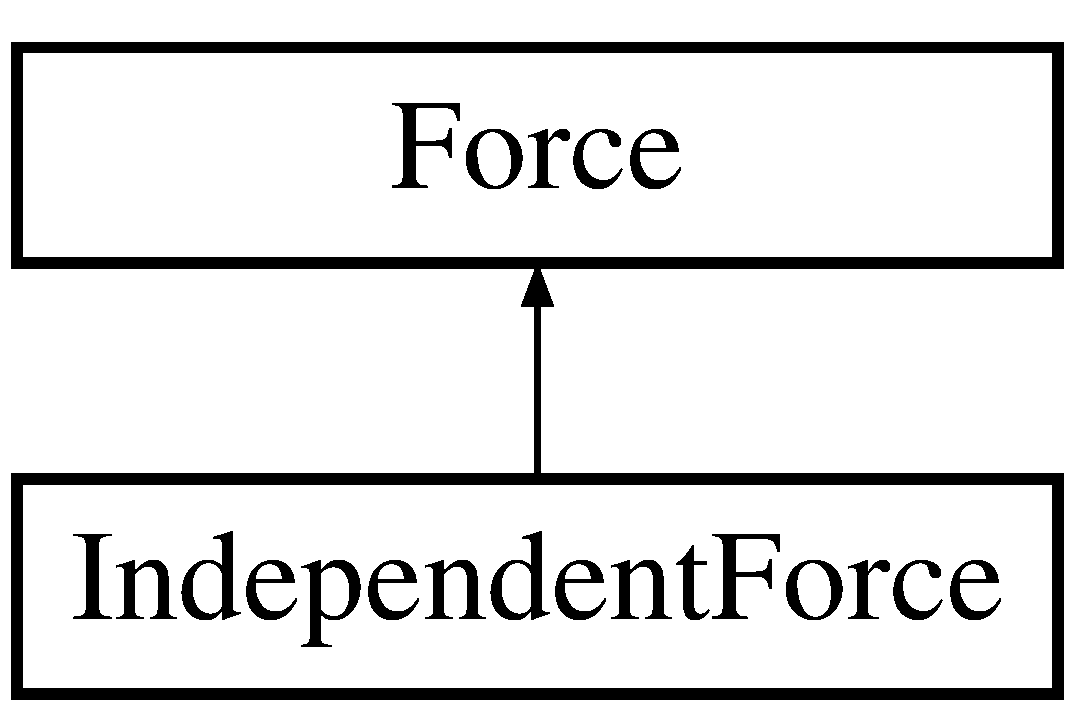
\includegraphics[height=2.000000cm]{class_independent_force}
\end{center}
\end{figure}
\subsection*{Public Member Functions}
\begin{DoxyCompactItemize}
\item 
\hyperlink{class_independent_force_a74333885143a3deed289d011642852d3}{Independent\-Force} (const \hyperlink{class_vector3_d}{Vector3\-D} \&f)
\item 
\hyperlink{class_vector3_d}{Vector3\-D} \hyperlink{class_independent_force_aeb5118d339cbe545db0bfbf47c4b5b68}{get} (float time) const 
\item 
\hyperlink{class_independent_force}{Independent\-Force} \& \hyperlink{class_independent_force_a07499f6810df352efaf432576b2fce1f}{operator+=} (const \hyperlink{class_independent_force}{Independent\-Force} \&rhs)
\end{DoxyCompactItemize}
\subsection*{Additional Inherited Members}


\subsection{Constructor \& Destructor Documentation}
\hypertarget{class_independent_force_a74333885143a3deed289d011642852d3}{\index{Independent\-Force@{Independent\-Force}!Independent\-Force@{Independent\-Force}}
\index{Independent\-Force@{Independent\-Force}!IndependentForce@{Independent\-Force}}
\subsubsection[{Independent\-Force}]{\setlength{\rightskip}{0pt plus 5cm}Independent\-Force\-::\-Independent\-Force (
\begin{DoxyParamCaption}
\item[{const {\bf Vector3\-D} \&}]{f}
\end{DoxyParamCaption}
)\hspace{0.3cm}{\ttfamily [inline]}}}\label{class_independent_force_a74333885143a3deed289d011642852d3}


\subsection{Member Function Documentation}
\hypertarget{class_independent_force_aeb5118d339cbe545db0bfbf47c4b5b68}{\index{Independent\-Force@{Independent\-Force}!get@{get}}
\index{get@{get}!IndependentForce@{Independent\-Force}}
\subsubsection[{get}]{\setlength{\rightskip}{0pt plus 5cm}{\bf Vector3\-D} Independent\-Force\-::get (
\begin{DoxyParamCaption}
\item[{float}]{time}
\end{DoxyParamCaption}
) const\hspace{0.3cm}{\ttfamily [inline]}, {\ttfamily [virtual]}}}\label{class_independent_force_aeb5118d339cbe545db0bfbf47c4b5b68}


Implements \hyperlink{class_force_afa6cdb1fe5f0d009e72fafa663147744}{Force}.

\hypertarget{class_independent_force_a07499f6810df352efaf432576b2fce1f}{\index{Independent\-Force@{Independent\-Force}!operator+=@{operator+=}}
\index{operator+=@{operator+=}!IndependentForce@{Independent\-Force}}
\subsubsection[{operator+=}]{\setlength{\rightskip}{0pt plus 5cm}{\bf Independent\-Force}\& Independent\-Force\-::operator+= (
\begin{DoxyParamCaption}
\item[{const {\bf Independent\-Force} \&}]{rhs}
\end{DoxyParamCaption}
)\hspace{0.3cm}{\ttfamily [inline]}}}\label{class_independent_force_a07499f6810df352efaf432576b2fce1f}


The documentation for this class was generated from the following file\-:\begin{DoxyCompactItemize}
\item 
D\-:/\-Development/\-My\-Projects/\-Physically\-Based\-Modeling/include/\hyperlink{_force_8h}{Force.\-h}\end{DoxyCompactItemize}

\hypertarget{class_matrix3_d}{\section{Matrix3\-D Class Reference}
\label{class_matrix3_d}\index{Matrix3\-D@{Matrix3\-D}}
}


{\ttfamily \#include $<$Utility.\-h$>$}

\subsection*{Public Member Functions}
\begin{DoxyCompactItemize}
\item 
\hyperlink{class_matrix3_d_afe9c6b7abe858fe9f6aea8f0607a00a7}{Matrix3\-D} ()
\item 
\hyperlink{class_matrix3_d_a3815dcfb26b7124d89a5c9f6b166ff5f}{Matrix3\-D} (double elem\mbox{[}row\-Size\mbox{]}\mbox{[}column\-Size\mbox{]})
\item 
\hyperlink{class_matrix3_d_a41fbb4c0c742c10a21343486a42a0e56}{Matrix3\-D} (double x, double y, double z)
\item 
void \hyperlink{class_matrix3_d_aec51075342822cfb4a2356ad6b970153}{set\-I\-D\-Mat} ()
\item 
void \hyperlink{class_matrix3_d_a6d9200e3ad1f997cb1bebcc9277f2b41}{get\-Elements} (double(\&e)\mbox{[}row\-Size\mbox{]}\mbox{[}column\-Size\mbox{]}) const 
\item 
double \hyperlink{class_matrix3_d_af226f6ecbf1240a56bd7f00c2a54f530}{get\-Elem} (int row, int column) const 
\item 
bool \hyperlink{class_matrix3_d_a0260b566bbd5579a3a2c393ef9c09eb0}{get\-Inversion} (\hyperlink{class_matrix3_d}{Matrix3\-D} \&inv\-Out)
\item 
\hyperlink{class_matrix3_d}{Matrix3\-D} \& \hyperlink{class_matrix3_d_a8049b657a2c0a150f95194a75e90789c}{operator=} (const \hyperlink{class_matrix3_d}{Matrix3\-D} \&rhs)
\item 
std\-::string \hyperlink{class_matrix3_d_a3f99e2bf75e31b08646b79b2c9756d14}{to\-String} () const 
\end{DoxyCompactItemize}
\subsection*{Friends}
\begin{DoxyCompactItemize}
\item 
\hyperlink{class_matrix3_d}{Matrix3\-D} \hyperlink{class_matrix3_d_a8aeebbc7c89ec0a85a08aee0d87c6aae}{operator$\ast$} (const \hyperlink{class_matrix3_d}{Matrix3\-D} \&s1, const \hyperlink{class_matrix3_d}{Matrix3\-D} \&s2)
\end{DoxyCompactItemize}


\subsection{Constructor \& Destructor Documentation}
\hypertarget{class_matrix3_d_afe9c6b7abe858fe9f6aea8f0607a00a7}{\index{Matrix3\-D@{Matrix3\-D}!Matrix3\-D@{Matrix3\-D}}
\index{Matrix3\-D@{Matrix3\-D}!Matrix3D@{Matrix3\-D}}
\subsubsection[{Matrix3\-D}]{\setlength{\rightskip}{0pt plus 5cm}Matrix3\-D\-::\-Matrix3\-D (
\begin{DoxyParamCaption}
{}
\end{DoxyParamCaption}
)}}\label{class_matrix3_d_afe9c6b7abe858fe9f6aea8f0607a00a7}
\hypertarget{class_matrix3_d_a3815dcfb26b7124d89a5c9f6b166ff5f}{\index{Matrix3\-D@{Matrix3\-D}!Matrix3\-D@{Matrix3\-D}}
\index{Matrix3\-D@{Matrix3\-D}!Matrix3D@{Matrix3\-D}}
\subsubsection[{Matrix3\-D}]{\setlength{\rightskip}{0pt plus 5cm}Matrix3\-D\-::\-Matrix3\-D (
\begin{DoxyParamCaption}
\item[{double}]{elem\mbox{[}row\-Size\mbox{]}\mbox{[}column\-Size\mbox{]}}
\end{DoxyParamCaption}
)}}\label{class_matrix3_d_a3815dcfb26b7124d89a5c9f6b166ff5f}
\hypertarget{class_matrix3_d_a41fbb4c0c742c10a21343486a42a0e56}{\index{Matrix3\-D@{Matrix3\-D}!Matrix3\-D@{Matrix3\-D}}
\index{Matrix3\-D@{Matrix3\-D}!Matrix3D@{Matrix3\-D}}
\subsubsection[{Matrix3\-D}]{\setlength{\rightskip}{0pt plus 5cm}Matrix3\-D\-::\-Matrix3\-D (
\begin{DoxyParamCaption}
\item[{double}]{x, }
\item[{double}]{y, }
\item[{double}]{z}
\end{DoxyParamCaption}
)}}\label{class_matrix3_d_a41fbb4c0c742c10a21343486a42a0e56}


\subsection{Member Function Documentation}
\hypertarget{class_matrix3_d_af226f6ecbf1240a56bd7f00c2a54f530}{\index{Matrix3\-D@{Matrix3\-D}!get\-Elem@{get\-Elem}}
\index{get\-Elem@{get\-Elem}!Matrix3D@{Matrix3\-D}}
\subsubsection[{get\-Elem}]{\setlength{\rightskip}{0pt plus 5cm}double Matrix3\-D\-::get\-Elem (
\begin{DoxyParamCaption}
\item[{int}]{row, }
\item[{int}]{column}
\end{DoxyParamCaption}
) const\hspace{0.3cm}{\ttfamily [inline]}}}\label{class_matrix3_d_af226f6ecbf1240a56bd7f00c2a54f530}
\hypertarget{class_matrix3_d_a6d9200e3ad1f997cb1bebcc9277f2b41}{\index{Matrix3\-D@{Matrix3\-D}!get\-Elements@{get\-Elements}}
\index{get\-Elements@{get\-Elements}!Matrix3D@{Matrix3\-D}}
\subsubsection[{get\-Elements}]{\setlength{\rightskip}{0pt plus 5cm}void Matrix3\-D\-::get\-Elements (
\begin{DoxyParamCaption}
\item[{double(\&)}]{e\mbox{[}row\-Size\mbox{]}\mbox{[}column\-Size\mbox{]}}
\end{DoxyParamCaption}
) const\hspace{0.3cm}{\ttfamily [inline]}}}\label{class_matrix3_d_a6d9200e3ad1f997cb1bebcc9277f2b41}
\hypertarget{class_matrix3_d_a0260b566bbd5579a3a2c393ef9c09eb0}{\index{Matrix3\-D@{Matrix3\-D}!get\-Inversion@{get\-Inversion}}
\index{get\-Inversion@{get\-Inversion}!Matrix3D@{Matrix3\-D}}
\subsubsection[{get\-Inversion}]{\setlength{\rightskip}{0pt plus 5cm}bool Matrix3\-D\-::get\-Inversion (
\begin{DoxyParamCaption}
\item[{{\bf Matrix3\-D} \&}]{inv\-Out}
\end{DoxyParamCaption}
)}}\label{class_matrix3_d_a0260b566bbd5579a3a2c393ef9c09eb0}
\hypertarget{class_matrix3_d_a8049b657a2c0a150f95194a75e90789c}{\index{Matrix3\-D@{Matrix3\-D}!operator=@{operator=}}
\index{operator=@{operator=}!Matrix3D@{Matrix3\-D}}
\subsubsection[{operator=}]{\setlength{\rightskip}{0pt plus 5cm}{\bf Matrix3\-D}\& Matrix3\-D\-::operator= (
\begin{DoxyParamCaption}
\item[{const {\bf Matrix3\-D} \&}]{rhs}
\end{DoxyParamCaption}
)}}\label{class_matrix3_d_a8049b657a2c0a150f95194a75e90789c}
\hypertarget{class_matrix3_d_aec51075342822cfb4a2356ad6b970153}{\index{Matrix3\-D@{Matrix3\-D}!set\-I\-D\-Mat@{set\-I\-D\-Mat}}
\index{set\-I\-D\-Mat@{set\-I\-D\-Mat}!Matrix3D@{Matrix3\-D}}
\subsubsection[{set\-I\-D\-Mat}]{\setlength{\rightskip}{0pt plus 5cm}void Matrix3\-D\-::set\-I\-D\-Mat (
\begin{DoxyParamCaption}
{}
\end{DoxyParamCaption}
)}}\label{class_matrix3_d_aec51075342822cfb4a2356ad6b970153}
\hypertarget{class_matrix3_d_a3f99e2bf75e31b08646b79b2c9756d14}{\index{Matrix3\-D@{Matrix3\-D}!to\-String@{to\-String}}
\index{to\-String@{to\-String}!Matrix3D@{Matrix3\-D}}
\subsubsection[{to\-String}]{\setlength{\rightskip}{0pt plus 5cm}std\-::string Matrix3\-D\-::to\-String (
\begin{DoxyParamCaption}
{}
\end{DoxyParamCaption}
) const}}\label{class_matrix3_d_a3f99e2bf75e31b08646b79b2c9756d14}


\subsection{Friends And Related Function Documentation}
\hypertarget{class_matrix3_d_a8aeebbc7c89ec0a85a08aee0d87c6aae}{\index{Matrix3\-D@{Matrix3\-D}!operator$\ast$@{operator$\ast$}}
\index{operator$\ast$@{operator$\ast$}!Matrix3D@{Matrix3\-D}}
\subsubsection[{operator$\ast$}]{\setlength{\rightskip}{0pt plus 5cm}{\bf Matrix3\-D} operator$\ast$ (
\begin{DoxyParamCaption}
\item[{const {\bf Matrix3\-D} \&}]{s1, }
\item[{const {\bf Matrix3\-D} \&}]{s2}
\end{DoxyParamCaption}
)\hspace{0.3cm}{\ttfamily [friend]}}}\label{class_matrix3_d_a8aeebbc7c89ec0a85a08aee0d87c6aae}


The documentation for this class was generated from the following file\-:\begin{DoxyCompactItemize}
\item 
D\-:/\-Development/\-My\-Projects/\-Physically\-Based\-Modeling/include/\hyperlink{_utility_8h}{Utility.\-h}\end{DoxyCompactItemize}

\hypertarget{class_object}{\section{Object Class Reference}
\label{class_object}\index{Object@{Object}}
}


{\ttfamily \#include $<$Object.\-h$>$}

Inheritance diagram for Object\-:\begin{figure}[H]
\begin{center}
\leavevmode
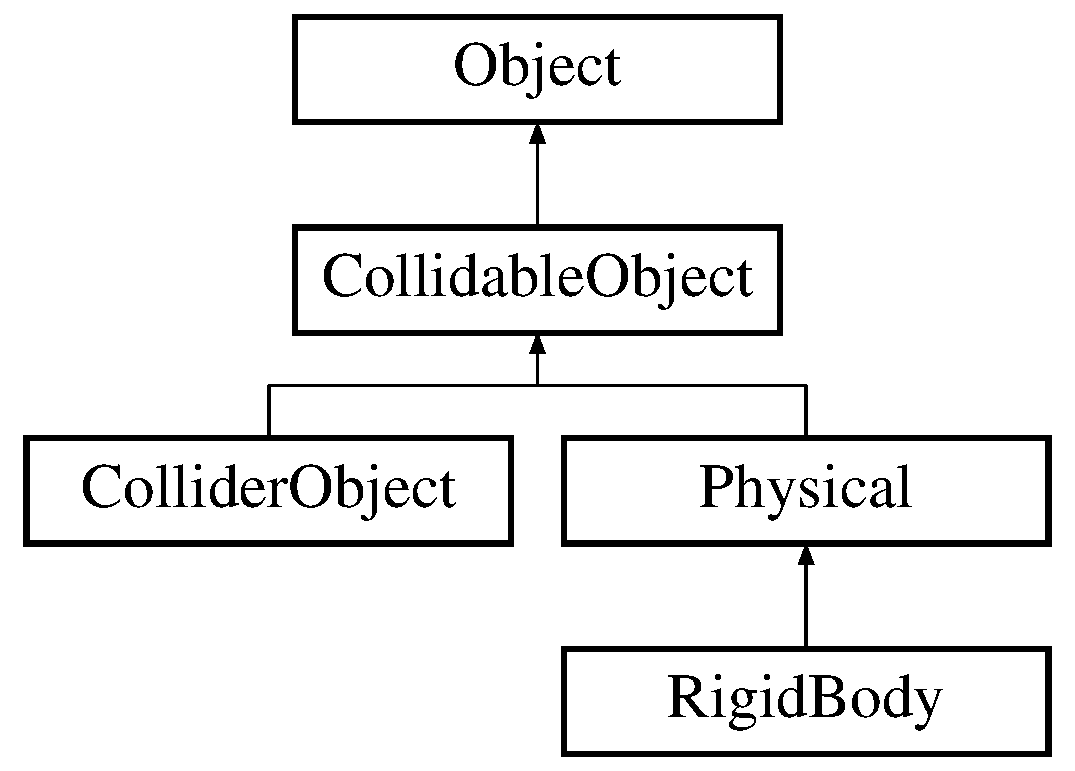
\includegraphics[height=4.000000cm]{class_object}
\end{center}
\end{figure}
\subsection*{Public Member Functions}
\begin{DoxyCompactItemize}
\item 
\hyperlink{class_object_af927ea9f0f93cd28814b76b41679246c}{Object} (const \hyperlink{class_vector3_d}{Vector3\-D} \&pos)
\item 
void \hyperlink{class_object_aad059ec469e812c147454f275709e88f}{set\-Renderable} (\hyperlink{class_renderable}{Renderable} $\ast$r)
\item 
const \hyperlink{class_renderable}{Renderable} $\ast$ \hyperlink{class_object_aed3cdc94cd166ca82b97da3e56aca49d}{get\-Renderable} () const 
\end{DoxyCompactItemize}
\subsection*{Public Attributes}
\begin{DoxyCompactItemize}
\item 
\hyperlink{class_transform}{Transform} \hyperlink{class_object_ad2104d9214add76b33191f1993faa3ae}{transform}
\end{DoxyCompactItemize}
\subsection*{Protected Attributes}
\begin{DoxyCompactItemize}
\item 
\hyperlink{class_renderable}{Renderable} $\ast$ \hyperlink{class_object_aa632828fdce73d2297c6b8841865f14d}{renderable}
\end{DoxyCompactItemize}


\subsection{Constructor \& Destructor Documentation}
\hypertarget{class_object_af927ea9f0f93cd28814b76b41679246c}{\index{Object@{Object}!Object@{Object}}
\index{Object@{Object}!Object@{Object}}
\subsubsection[{Object}]{\setlength{\rightskip}{0pt plus 5cm}Object\-::\-Object (
\begin{DoxyParamCaption}
\item[{const {\bf Vector3\-D} \&}]{pos}
\end{DoxyParamCaption}
)\hspace{0.3cm}{\ttfamily [inline]}}}\label{class_object_af927ea9f0f93cd28814b76b41679246c}


\subsection{Member Function Documentation}
\hypertarget{class_object_aed3cdc94cd166ca82b97da3e56aca49d}{\index{Object@{Object}!get\-Renderable@{get\-Renderable}}
\index{get\-Renderable@{get\-Renderable}!Object@{Object}}
\subsubsection[{get\-Renderable}]{\setlength{\rightskip}{0pt plus 5cm}const {\bf Renderable}$\ast$ Object\-::get\-Renderable (
\begin{DoxyParamCaption}
{}
\end{DoxyParamCaption}
) const\hspace{0.3cm}{\ttfamily [inline]}}}\label{class_object_aed3cdc94cd166ca82b97da3e56aca49d}
\hypertarget{class_object_aad059ec469e812c147454f275709e88f}{\index{Object@{Object}!set\-Renderable@{set\-Renderable}}
\index{set\-Renderable@{set\-Renderable}!Object@{Object}}
\subsubsection[{set\-Renderable}]{\setlength{\rightskip}{0pt plus 5cm}void Object\-::set\-Renderable (
\begin{DoxyParamCaption}
\item[{{\bf Renderable} $\ast$}]{r}
\end{DoxyParamCaption}
)\hspace{0.3cm}{\ttfamily [inline]}}}\label{class_object_aad059ec469e812c147454f275709e88f}


\subsection{Member Data Documentation}
\hypertarget{class_object_aa632828fdce73d2297c6b8841865f14d}{\index{Object@{Object}!renderable@{renderable}}
\index{renderable@{renderable}!Object@{Object}}
\subsubsection[{renderable}]{\setlength{\rightskip}{0pt plus 5cm}{\bf Renderable}$\ast$ Object\-::renderable\hspace{0.3cm}{\ttfamily [protected]}}}\label{class_object_aa632828fdce73d2297c6b8841865f14d}
\hypertarget{class_object_ad2104d9214add76b33191f1993faa3ae}{\index{Object@{Object}!transform@{transform}}
\index{transform@{transform}!Object@{Object}}
\subsubsection[{transform}]{\setlength{\rightskip}{0pt plus 5cm}{\bf Transform} Object\-::transform}}\label{class_object_ad2104d9214add76b33191f1993faa3ae}


The documentation for this class was generated from the following file\-:\begin{DoxyCompactItemize}
\item 
D\-:/\-Development/\-My\-Projects/\-Physically\-Based\-Modeling/include/\hyperlink{_object_8h}{Object.\-h}\end{DoxyCompactItemize}

\hypertarget{class_p_b_time}{\section{P\-B\-Time Class Reference}
\label{class_p_b_time}\index{P\-B\-Time@{P\-B\-Time}}
}


{\ttfamily \#include $<$Physically\-Based.\-h$>$}

\subsection*{Public Member Functions}
\begin{DoxyCompactItemize}
\item 
\hyperlink{class_p_b_time_a09bdd4a9e468b5582f0c675ad6237c4e}{P\-B\-Time} ()
\item 
\hyperlink{class_p_b_time_a695ca9cad69059a0793b4b3c69e25151}{P\-B\-Time} (float timestep, float elapsed\-Time)
\item 
float \hyperlink{class_p_b_time_a1bf628d33c9577d5f6b51c2394dbe3a5}{get\-Timestep} () const 
\item 
float \hyperlink{class_p_b_time_abbb62704149b7c9069d120e32333700e}{get\-Elapsed\-Time} () const 
\item 
void \hyperlink{class_p_b_time_a31494e412baefed4c000747ae7604eb5}{set\-Timestep} (float t)
\item 
void \hyperlink{class_p_b_time_a46d60a843cf2e910854ab9fb491e783a}{set\-Elapsed\-Time} (float ct)
\end{DoxyCompactItemize}
\subsection*{Friends}
\begin{DoxyCompactItemize}
\item 
class \hyperlink{class_p_b_time_aeee6bd23afed3d408fb21a7d857a8f3b}{Physically\-Based}
\end{DoxyCompactItemize}


\subsection{Constructor \& Destructor Documentation}
\hypertarget{class_p_b_time_a09bdd4a9e468b5582f0c675ad6237c4e}{\index{P\-B\-Time@{P\-B\-Time}!P\-B\-Time@{P\-B\-Time}}
\index{P\-B\-Time@{P\-B\-Time}!PBTime@{P\-B\-Time}}
\subsubsection[{P\-B\-Time}]{\setlength{\rightskip}{0pt plus 5cm}P\-B\-Time\-::\-P\-B\-Time (
\begin{DoxyParamCaption}
{}
\end{DoxyParamCaption}
)\hspace{0.3cm}{\ttfamily [inline]}}}\label{class_p_b_time_a09bdd4a9e468b5582f0c675ad6237c4e}
\hypertarget{class_p_b_time_a695ca9cad69059a0793b4b3c69e25151}{\index{P\-B\-Time@{P\-B\-Time}!P\-B\-Time@{P\-B\-Time}}
\index{P\-B\-Time@{P\-B\-Time}!PBTime@{P\-B\-Time}}
\subsubsection[{P\-B\-Time}]{\setlength{\rightskip}{0pt plus 5cm}P\-B\-Time\-::\-P\-B\-Time (
\begin{DoxyParamCaption}
\item[{float}]{timestep, }
\item[{float}]{elapsed\-Time}
\end{DoxyParamCaption}
)\hspace{0.3cm}{\ttfamily [inline]}}}\label{class_p_b_time_a695ca9cad69059a0793b4b3c69e25151}


\subsection{Member Function Documentation}
\hypertarget{class_p_b_time_abbb62704149b7c9069d120e32333700e}{\index{P\-B\-Time@{P\-B\-Time}!get\-Elapsed\-Time@{get\-Elapsed\-Time}}
\index{get\-Elapsed\-Time@{get\-Elapsed\-Time}!PBTime@{P\-B\-Time}}
\subsubsection[{get\-Elapsed\-Time}]{\setlength{\rightskip}{0pt plus 5cm}float P\-B\-Time\-::get\-Elapsed\-Time (
\begin{DoxyParamCaption}
{}
\end{DoxyParamCaption}
) const\hspace{0.3cm}{\ttfamily [inline]}}}\label{class_p_b_time_abbb62704149b7c9069d120e32333700e}
\hypertarget{class_p_b_time_a1bf628d33c9577d5f6b51c2394dbe3a5}{\index{P\-B\-Time@{P\-B\-Time}!get\-Timestep@{get\-Timestep}}
\index{get\-Timestep@{get\-Timestep}!PBTime@{P\-B\-Time}}
\subsubsection[{get\-Timestep}]{\setlength{\rightskip}{0pt plus 5cm}float P\-B\-Time\-::get\-Timestep (
\begin{DoxyParamCaption}
{}
\end{DoxyParamCaption}
) const\hspace{0.3cm}{\ttfamily [inline]}}}\label{class_p_b_time_a1bf628d33c9577d5f6b51c2394dbe3a5}
\hypertarget{class_p_b_time_a46d60a843cf2e910854ab9fb491e783a}{\index{P\-B\-Time@{P\-B\-Time}!set\-Elapsed\-Time@{set\-Elapsed\-Time}}
\index{set\-Elapsed\-Time@{set\-Elapsed\-Time}!PBTime@{P\-B\-Time}}
\subsubsection[{set\-Elapsed\-Time}]{\setlength{\rightskip}{0pt plus 5cm}void P\-B\-Time\-::set\-Elapsed\-Time (
\begin{DoxyParamCaption}
\item[{float}]{ct}
\end{DoxyParamCaption}
)\hspace{0.3cm}{\ttfamily [inline]}}}\label{class_p_b_time_a46d60a843cf2e910854ab9fb491e783a}
\hypertarget{class_p_b_time_a31494e412baefed4c000747ae7604eb5}{\index{P\-B\-Time@{P\-B\-Time}!set\-Timestep@{set\-Timestep}}
\index{set\-Timestep@{set\-Timestep}!PBTime@{P\-B\-Time}}
\subsubsection[{set\-Timestep}]{\setlength{\rightskip}{0pt plus 5cm}void P\-B\-Time\-::set\-Timestep (
\begin{DoxyParamCaption}
\item[{float}]{t}
\end{DoxyParamCaption}
)\hspace{0.3cm}{\ttfamily [inline]}}}\label{class_p_b_time_a31494e412baefed4c000747ae7604eb5}


\subsection{Friends And Related Function Documentation}
\hypertarget{class_p_b_time_aeee6bd23afed3d408fb21a7d857a8f3b}{\index{P\-B\-Time@{P\-B\-Time}!Physically\-Based@{Physically\-Based}}
\index{Physically\-Based@{Physically\-Based}!PBTime@{P\-B\-Time}}
\subsubsection[{Physically\-Based}]{\setlength{\rightskip}{0pt plus 5cm}friend class Physically\-Based\hspace{0.3cm}{\ttfamily [friend]}}}\label{class_p_b_time_aeee6bd23afed3d408fb21a7d857a8f3b}


The documentation for this class was generated from the following file\-:\begin{DoxyCompactItemize}
\item 
D\-:/\-Development/\-My\-Projects/\-Physically\-Based\-Modeling/include/\hyperlink{_physically_based_8h}{Physically\-Based.\-h}\end{DoxyCompactItemize}

\hypertarget{class_ui_1_1_phys_b_dock}{\section{Ui\-:\-:Phys\-B\-Dock Class Reference}
\label{class_ui_1_1_phys_b_dock}\index{Ui\-::\-Phys\-B\-Dock@{Ui\-::\-Phys\-B\-Dock}}
}


{\ttfamily \#include $<$ui\-\_\-\-Physically\-Based.\-h$>$}

Inheritance diagram for Ui\-:\-:Phys\-B\-Dock\-:\begin{figure}[H]
\begin{center}
\leavevmode
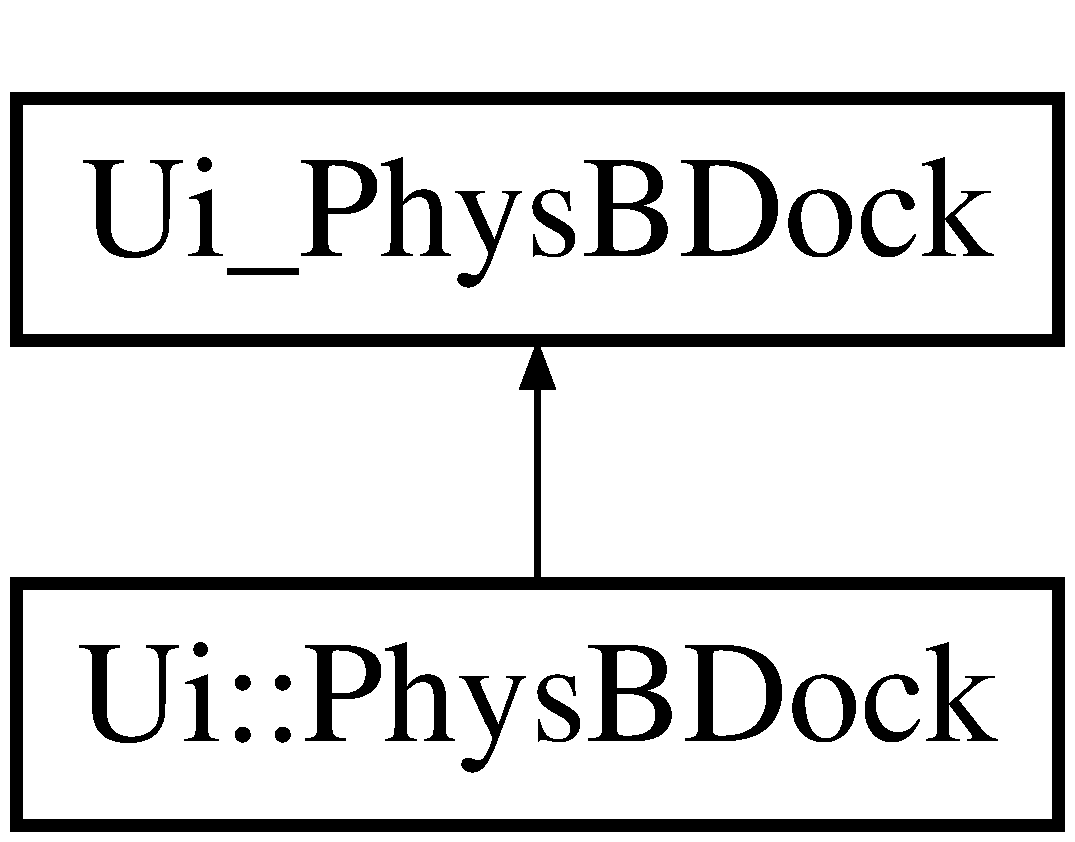
\includegraphics[height=2.000000cm]{class_ui_1_1_phys_b_dock}
\end{center}
\end{figure}
\subsection*{Additional Inherited Members}


The documentation for this class was generated from the following file\-:\begin{DoxyCompactItemize}
\item 
D\-:/\-Development/\-My\-Projects/\-Physically\-Based\-Modeling/include/\hyperlink{ui___physically_based_8h}{ui\-\_\-\-Physically\-Based.\-h}\end{DoxyCompactItemize}

\hypertarget{class_phys_b_event}{\section{Phys\-B\-Event Class Reference}
\label{class_phys_b_event}\index{Phys\-B\-Event@{Phys\-B\-Event}}
}


{\ttfamily \#include $<$Events.\-h$>$}

Inheritance diagram for Phys\-B\-Event\-:\begin{figure}[H]
\begin{center}
\leavevmode
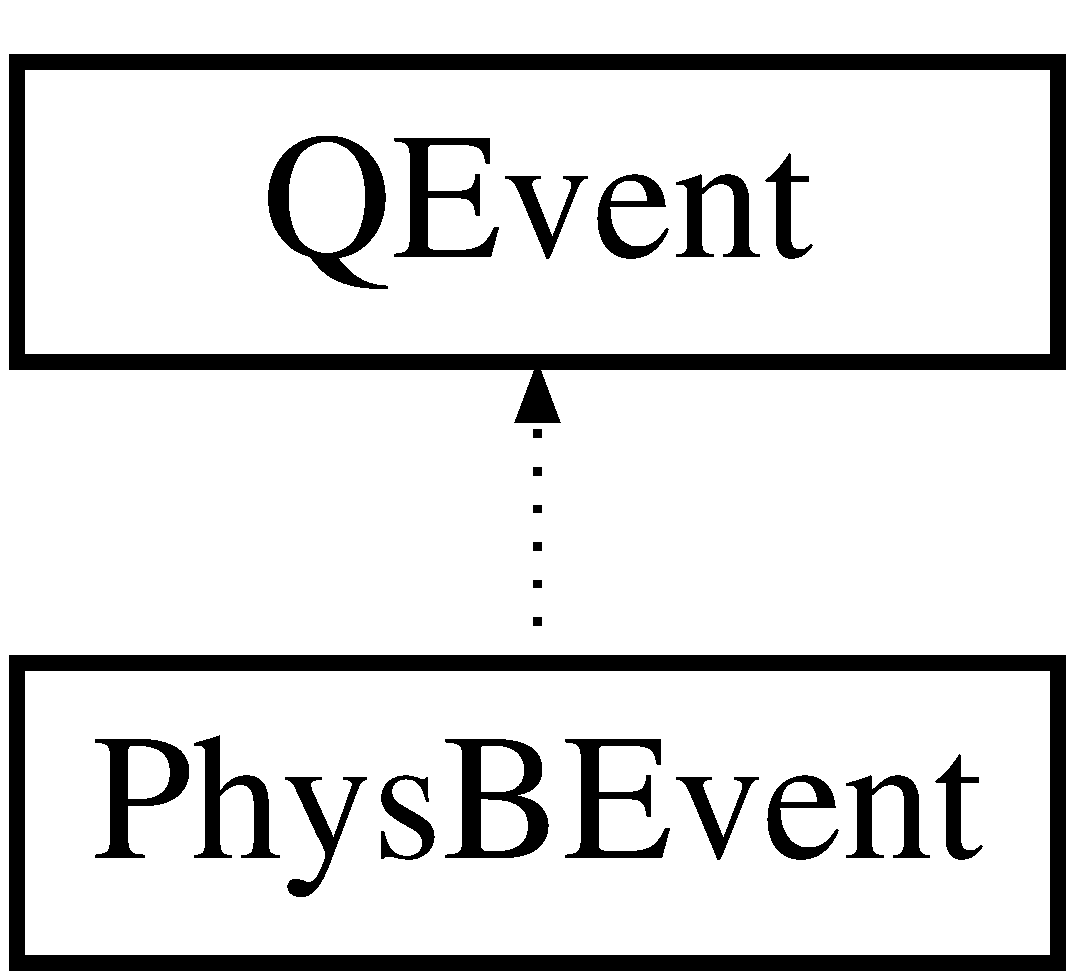
\includegraphics[height=2.000000cm]{class_phys_b_event}
\end{center}
\end{figure}
\subsection*{Static Public Attributes}
\begin{DoxyCompactItemize}
\item 
static const Q\-Event\-::\-Type \hyperlink{class_phys_b_event_a7ab5c424201f6461af7721d81310968c}{trace\-Start} = static\-\_\-cast$<$Q\-Event\-::\-Type$>$(1234)
\item 
static const Q\-Event\-::\-Type \hyperlink{class_phys_b_event_a56d494f3a63d0b992c8083a3fb3a8a4c}{trace\-End} = static\-\_\-cast$<$Q\-Event\-::\-Type$>$(1235)
\item 
static const Q\-Event\-::\-Type \hyperlink{class_phys_b_event_a189bab4e3463356d8ef0020562a0ea53}{trace\-Pixel\-Filled} = static\-\_\-cast$<$Q\-Event\-::\-Type$>$(1236)
\end{DoxyCompactItemize}


\subsection{Member Data Documentation}
\hypertarget{class_phys_b_event_a56d494f3a63d0b992c8083a3fb3a8a4c}{\index{Phys\-B\-Event@{Phys\-B\-Event}!trace\-End@{trace\-End}}
\index{trace\-End@{trace\-End}!PhysBEvent@{Phys\-B\-Event}}
\subsubsection[{trace\-End}]{\setlength{\rightskip}{0pt plus 5cm}const Q\-Event\-::\-Type Phys\-B\-Event\-::trace\-End = static\-\_\-cast$<$Q\-Event\-::\-Type$>$(1235)\hspace{0.3cm}{\ttfamily [static]}}}\label{class_phys_b_event_a56d494f3a63d0b992c8083a3fb3a8a4c}
\hypertarget{class_phys_b_event_a189bab4e3463356d8ef0020562a0ea53}{\index{Phys\-B\-Event@{Phys\-B\-Event}!trace\-Pixel\-Filled@{trace\-Pixel\-Filled}}
\index{trace\-Pixel\-Filled@{trace\-Pixel\-Filled}!PhysBEvent@{Phys\-B\-Event}}
\subsubsection[{trace\-Pixel\-Filled}]{\setlength{\rightskip}{0pt plus 5cm}const Q\-Event\-::\-Type Phys\-B\-Event\-::trace\-Pixel\-Filled = static\-\_\-cast$<$Q\-Event\-::\-Type$>$(1236)\hspace{0.3cm}{\ttfamily [static]}}}\label{class_phys_b_event_a189bab4e3463356d8ef0020562a0ea53}
\hypertarget{class_phys_b_event_a7ab5c424201f6461af7721d81310968c}{\index{Phys\-B\-Event@{Phys\-B\-Event}!trace\-Start@{trace\-Start}}
\index{trace\-Start@{trace\-Start}!PhysBEvent@{Phys\-B\-Event}}
\subsubsection[{trace\-Start}]{\setlength{\rightskip}{0pt plus 5cm}const Q\-Event\-::\-Type Phys\-B\-Event\-::trace\-Start = static\-\_\-cast$<$Q\-Event\-::\-Type$>$(1234)\hspace{0.3cm}{\ttfamily [static]}}}\label{class_phys_b_event_a7ab5c424201f6461af7721d81310968c}


The documentation for this class was generated from the following file\-:\begin{DoxyCompactItemize}
\item 
D\-:/\-Development/\-My\-Projects/\-Physically\-Based\-Modeling/include/\hyperlink{_events_8h}{Events.\-h}\end{DoxyCompactItemize}

\hypertarget{class_physical}{\section{Physical Class Reference}
\label{class_physical}\index{Physical@{Physical}}
}


{\ttfamily \#include $<$Physical.\-h$>$}

Inheritance diagram for Physical\-:\begin{figure}[H]
\begin{center}
\leavevmode
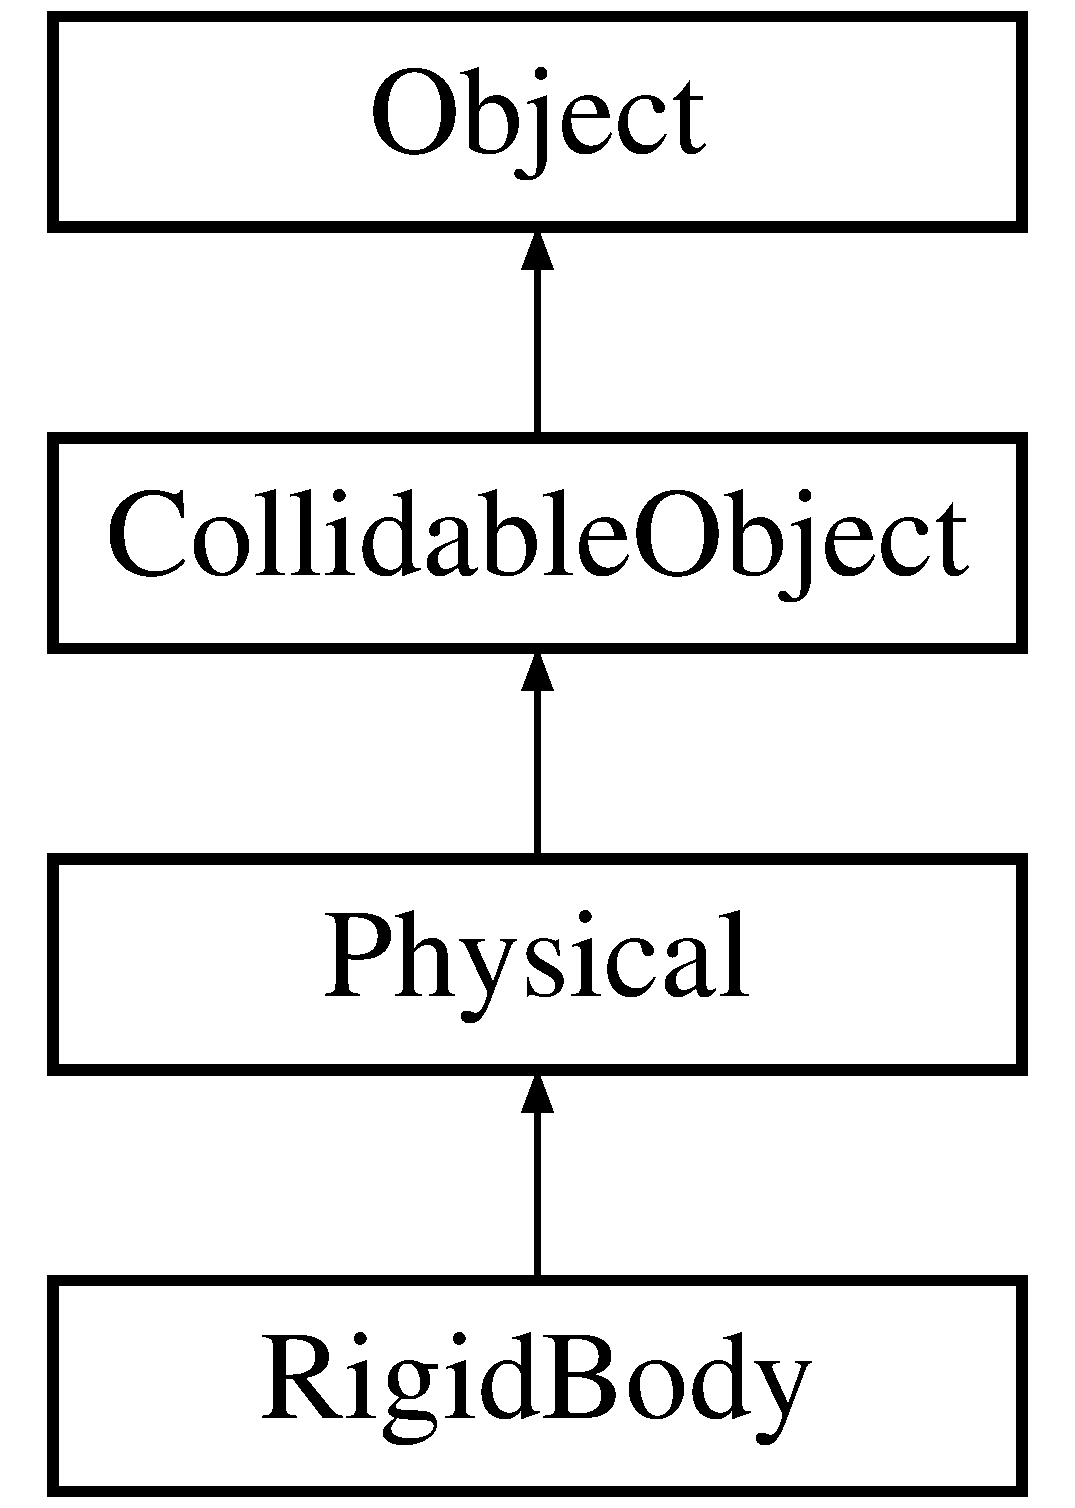
\includegraphics[height=4.000000cm]{class_physical}
\end{center}
\end{figure}
\subsection*{Public Member Functions}
\begin{DoxyCompactItemize}
\item 
void \hyperlink{class_physical_a61419e993f622482a2c2ae4614a16944}{update} (const \hyperlink{class_p_b_time}{P\-B\-Time} \&\hyperlink{_physically_based_8h_a766da334af281a8fa1ed5cf404d0ec45}{the\-Time}, const std\-::vector$<$ \hyperlink{class_force}{Force} $>$ \&forces, const std\-::vector$<$ \hyperlink{class_force}{Force} $>$ \&accels)
\item 
\hyperlink{class_physical}{Physical} $\ast$ \hyperlink{class_physical_a3ba7964e2b399a96b5c306328ff9367d}{get\-Updated} (const \hyperlink{class_p_b_time}{P\-B\-Time} \&\hyperlink{_physically_based_8h_a766da334af281a8fa1ed5cf404d0ec45}{the\-Time}, const std\-::vector$<$ \hyperlink{class_force}{Force} $>$ \&forces, const std\-::vector$<$ \hyperlink{class_force}{Force} $>$ \&accels)
\item 
virtual \hyperlink{class_deferred_force}{Deferred\-Force} $\ast$ \hyperlink{class_physical_aaa95a85d67ec076d41a301e546661452}{get\-Collision\-Force} ()=0
\end{DoxyCompactItemize}
\subsection*{Protected Member Functions}
\begin{DoxyCompactItemize}
\item 
\hyperlink{class_physical_ac11a1bca87389886d9d8291fef41ad8c}{Physical} ()
\item 
virtual void \hyperlink{class_physical_ac2f0c203798c646a9bffc9ef2bb64185}{update} (const \hyperlink{class_p_b_time}{P\-B\-Time} \&\hyperlink{_physically_based_8h_a766da334af281a8fa1ed5cf404d0ec45}{the\-Time}, \hyperlink{class_collidable_object}{Collidable\-Object} \&co)
\item 
virtual void \hyperlink{class_physical_a4aae3956fcf233e43d0bd65d942c4d7b}{update} (const \hyperlink{class_p_b_time}{P\-B\-Time} \&\hyperlink{_physically_based_8h_a766da334af281a8fa1ed5cf404d0ec45}{the\-Time}, \hyperlink{class_physical}{Physical} \&p, const std\-::vector$<$ \hyperlink{class_force}{Force} $>$ \&forces, const std\-::vector$<$ \hyperlink{class_force}{Force} $>$ \&accels)=0
\item 
virtual \hyperlink{class_physical}{Physical} $\ast$ \hyperlink{class_physical_a8e6b99aec0d99df8e330881a25d936e6}{clone} () const =0
\end{DoxyCompactItemize}
\subsection*{Additional Inherited Members}


\subsection{Constructor \& Destructor Documentation}
\hypertarget{class_physical_ac11a1bca87389886d9d8291fef41ad8c}{\index{Physical@{Physical}!Physical@{Physical}}
\index{Physical@{Physical}!Physical@{Physical}}
\subsubsection[{Physical}]{\setlength{\rightskip}{0pt plus 5cm}Physical\-::\-Physical (
\begin{DoxyParamCaption}
{}
\end{DoxyParamCaption}
)\hspace{0.3cm}{\ttfamily [inline]}, {\ttfamily [protected]}}}\label{class_physical_ac11a1bca87389886d9d8291fef41ad8c}


\subsection{Member Function Documentation}
\hypertarget{class_physical_a8e6b99aec0d99df8e330881a25d936e6}{\index{Physical@{Physical}!clone@{clone}}
\index{clone@{clone}!Physical@{Physical}}
\subsubsection[{clone}]{\setlength{\rightskip}{0pt plus 5cm}virtual {\bf Physical}$\ast$ Physical\-::clone (
\begin{DoxyParamCaption}
{}
\end{DoxyParamCaption}
) const\hspace{0.3cm}{\ttfamily [protected]}, {\ttfamily [pure virtual]}}}\label{class_physical_a8e6b99aec0d99df8e330881a25d936e6}


Implements \hyperlink{class_collidable_object_af7d1cf4164b033a6e68c5988d4b8aeb8}{Collidable\-Object}.

\hypertarget{class_physical_aaa95a85d67ec076d41a301e546661452}{\index{Physical@{Physical}!get\-Collision\-Force@{get\-Collision\-Force}}
\index{get\-Collision\-Force@{get\-Collision\-Force}!Physical@{Physical}}
\subsubsection[{get\-Collision\-Force}]{\setlength{\rightskip}{0pt plus 5cm}virtual {\bf Deferred\-Force}$\ast$ Physical\-::get\-Collision\-Force (
\begin{DoxyParamCaption}
{}
\end{DoxyParamCaption}
)\hspace{0.3cm}{\ttfamily [pure virtual]}}}\label{class_physical_aaa95a85d67ec076d41a301e546661452}
\hypertarget{class_physical_a3ba7964e2b399a96b5c306328ff9367d}{\index{Physical@{Physical}!get\-Updated@{get\-Updated}}
\index{get\-Updated@{get\-Updated}!Physical@{Physical}}
\subsubsection[{get\-Updated}]{\setlength{\rightskip}{0pt plus 5cm}{\bf Physical}$\ast$ Physical\-::get\-Updated (
\begin{DoxyParamCaption}
\item[{const {\bf P\-B\-Time} \&}]{the\-Time, }
\item[{const std\-::vector$<$ {\bf Force} $>$ \&}]{forces, }
\item[{const std\-::vector$<$ {\bf Force} $>$ \&}]{accels}
\end{DoxyParamCaption}
)\hspace{0.3cm}{\ttfamily [inline]}}}\label{class_physical_a3ba7964e2b399a96b5c306328ff9367d}
\hypertarget{class_physical_a61419e993f622482a2c2ae4614a16944}{\index{Physical@{Physical}!update@{update}}
\index{update@{update}!Physical@{Physical}}
\subsubsection[{update}]{\setlength{\rightskip}{0pt plus 5cm}void Physical\-::update (
\begin{DoxyParamCaption}
\item[{const {\bf P\-B\-Time} \&}]{the\-Time, }
\item[{const std\-::vector$<$ {\bf Force} $>$ \&}]{forces, }
\item[{const std\-::vector$<$ {\bf Force} $>$ \&}]{accels}
\end{DoxyParamCaption}
)\hspace{0.3cm}{\ttfamily [inline]}}}\label{class_physical_a61419e993f622482a2c2ae4614a16944}
\hypertarget{class_physical_ac2f0c203798c646a9bffc9ef2bb64185}{\index{Physical@{Physical}!update@{update}}
\index{update@{update}!Physical@{Physical}}
\subsubsection[{update}]{\setlength{\rightskip}{0pt plus 5cm}virtual void Physical\-::update (
\begin{DoxyParamCaption}
\item[{const {\bf P\-B\-Time} \&}]{the\-Time, }
\item[{{\bf Collidable\-Object} \&}]{co}
\end{DoxyParamCaption}
)\hspace{0.3cm}{\ttfamily [inline]}, {\ttfamily [protected]}, {\ttfamily [virtual]}}}\label{class_physical_ac2f0c203798c646a9bffc9ef2bb64185}


Implements \hyperlink{class_collidable_object_a20734a532bf708d8fb5856483d5b8ed2}{Collidable\-Object}.

\hypertarget{class_physical_a4aae3956fcf233e43d0bd65d942c4d7b}{\index{Physical@{Physical}!update@{update}}
\index{update@{update}!Physical@{Physical}}
\subsubsection[{update}]{\setlength{\rightskip}{0pt plus 5cm}virtual void Physical\-::update (
\begin{DoxyParamCaption}
\item[{const {\bf P\-B\-Time} \&}]{the\-Time, }
\item[{{\bf Physical} \&}]{p, }
\item[{const std\-::vector$<$ {\bf Force} $>$ \&}]{forces, }
\item[{const std\-::vector$<$ {\bf Force} $>$ \&}]{accels}
\end{DoxyParamCaption}
)\hspace{0.3cm}{\ttfamily [protected]}, {\ttfamily [pure virtual]}}}\label{class_physical_a4aae3956fcf233e43d0bd65d942c4d7b}


The documentation for this class was generated from the following file\-:\begin{DoxyCompactItemize}
\item 
D\-:/\-Development/\-My\-Projects/\-Physically\-Based\-Modeling/include/\hyperlink{_physical_8h}{Physical.\-h}\end{DoxyCompactItemize}

\hypertarget{class_q_s_f_m_l_canvas}{\section{Q\-S\-F\-M\-L\-Canvas Class Reference}
\label{class_q_s_f_m_l_canvas}\index{Q\-S\-F\-M\-L\-Canvas@{Q\-S\-F\-M\-L\-Canvas}}
}


{\ttfamily \#include $<$Q\-S\-F\-M\-L\-Canvas.\-h$>$}

Inheritance diagram for Q\-S\-F\-M\-L\-Canvas\-:\begin{figure}[H]
\begin{center}
\leavevmode
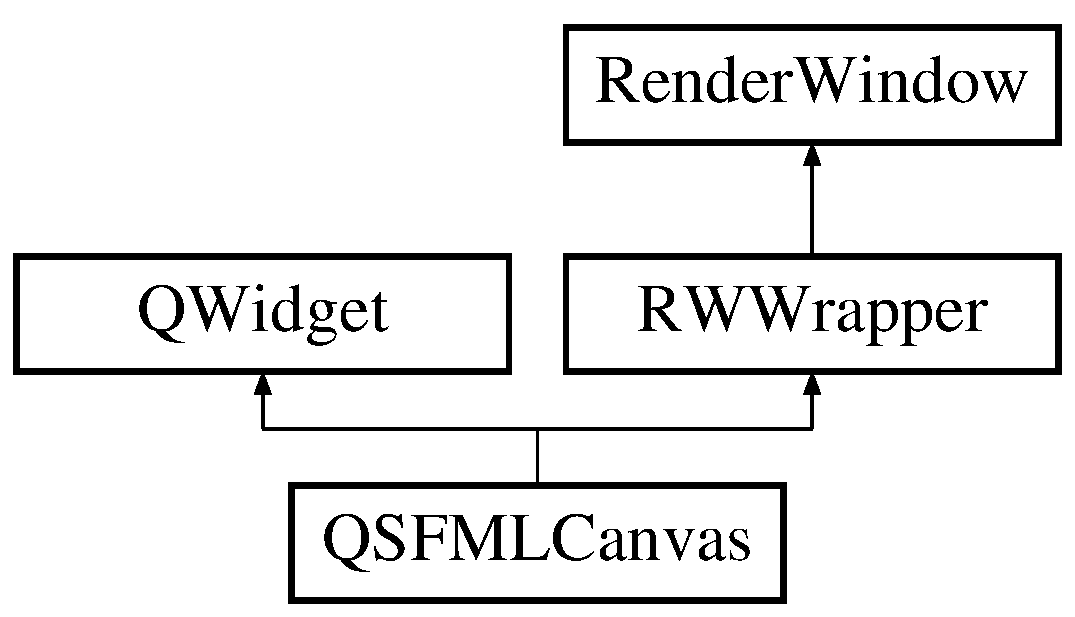
\includegraphics[height=3.000000cm]{class_q_s_f_m_l_canvas}
\end{center}
\end{figure}
\subsection*{Public Member Functions}
\begin{DoxyCompactItemize}
\item 
\hyperlink{class_q_s_f_m_l_canvas_ab183b3e99289e9a66d940dd9d1ae4d30}{Q\-S\-F\-M\-L\-Canvas} (Q\-Widget $\ast$Parent, const Q\-Point \&Position, const Q\-Size \&Size, unsigned int Frame\-Time)
\item 
virtual \hyperlink{class_q_s_f_m_l_canvas_acd0248c62e51d6f8b5c206395a417433}{$\sim$\-Q\-S\-F\-M\-L\-Canvas} ()
\item 
void \hyperlink{class_q_s_f_m_l_canvas_a971c183ca239ef73122de55957ec377b}{add\-Object} (const \hyperlink{class_object}{Object} $\ast$o)
\end{DoxyCompactItemize}


\subsection{Constructor \& Destructor Documentation}
\hypertarget{class_q_s_f_m_l_canvas_ab183b3e99289e9a66d940dd9d1ae4d30}{\index{Q\-S\-F\-M\-L\-Canvas@{Q\-S\-F\-M\-L\-Canvas}!Q\-S\-F\-M\-L\-Canvas@{Q\-S\-F\-M\-L\-Canvas}}
\index{Q\-S\-F\-M\-L\-Canvas@{Q\-S\-F\-M\-L\-Canvas}!QSFMLCanvas@{Q\-S\-F\-M\-L\-Canvas}}
\subsubsection[{Q\-S\-F\-M\-L\-Canvas}]{\setlength{\rightskip}{0pt plus 5cm}Q\-S\-F\-M\-L\-Canvas\-::\-Q\-S\-F\-M\-L\-Canvas (
\begin{DoxyParamCaption}
\item[{Q\-Widget $\ast$}]{Parent, }
\item[{const Q\-Point \&}]{Position, }
\item[{const Q\-Size \&}]{Size, }
\item[{unsigned int}]{Frame\-Time}
\end{DoxyParamCaption}
)}}\label{class_q_s_f_m_l_canvas_ab183b3e99289e9a66d940dd9d1ae4d30}

\begin{DoxyParams}{Parameters}
{\em Parent} & \-: Parent of the widget \\
\hline
{\em Position} & \-: Position of the widget \\
\hline
{\em Size} & \-: Size of the widget \\
\hline
\end{DoxyParams}
\hypertarget{class_q_s_f_m_l_canvas_acd0248c62e51d6f8b5c206395a417433}{\index{Q\-S\-F\-M\-L\-Canvas@{Q\-S\-F\-M\-L\-Canvas}!$\sim$\-Q\-S\-F\-M\-L\-Canvas@{$\sim$\-Q\-S\-F\-M\-L\-Canvas}}
\index{$\sim$\-Q\-S\-F\-M\-L\-Canvas@{$\sim$\-Q\-S\-F\-M\-L\-Canvas}!QSFMLCanvas@{Q\-S\-F\-M\-L\-Canvas}}
\subsubsection[{$\sim$\-Q\-S\-F\-M\-L\-Canvas}]{\setlength{\rightskip}{0pt plus 5cm}virtual Q\-S\-F\-M\-L\-Canvas\-::$\sim$\-Q\-S\-F\-M\-L\-Canvas (
\begin{DoxyParamCaption}
{}
\end{DoxyParamCaption}
)\hspace{0.3cm}{\ttfamily [virtual]}}}\label{class_q_s_f_m_l_canvas_acd0248c62e51d6f8b5c206395a417433}


\subsection{Member Function Documentation}
\hypertarget{class_q_s_f_m_l_canvas_a971c183ca239ef73122de55957ec377b}{\index{Q\-S\-F\-M\-L\-Canvas@{Q\-S\-F\-M\-L\-Canvas}!add\-Object@{add\-Object}}
\index{add\-Object@{add\-Object}!QSFMLCanvas@{Q\-S\-F\-M\-L\-Canvas}}
\subsubsection[{add\-Object}]{\setlength{\rightskip}{0pt plus 5cm}void Q\-S\-F\-M\-L\-Canvas\-::add\-Object (
\begin{DoxyParamCaption}
\item[{const {\bf Object} $\ast$}]{o}
\end{DoxyParamCaption}
)\hspace{0.3cm}{\ttfamily [inline]}}}\label{class_q_s_f_m_l_canvas_a971c183ca239ef73122de55957ec377b}


The documentation for this class was generated from the following file\-:\begin{DoxyCompactItemize}
\item 
D\-:/\-Development/\-My\-Projects/\-Physically\-Based\-Modeling/include/\-G\-U\-I/\hyperlink{_q_s_f_m_l_canvas_8h}{Q\-S\-F\-M\-L\-Canvas.\-h}\end{DoxyCompactItemize}

\hypertarget{class_quad_plane}{\section{Quad\-Plane Class Reference}
\label{class_quad_plane}\index{Quad\-Plane@{Quad\-Plane}}
}


{\ttfamily \#include $<$Quad\-Plane.\-h$>$}

Inheritance diagram for Quad\-Plane\-:\begin{figure}[H]
\begin{center}
\leavevmode
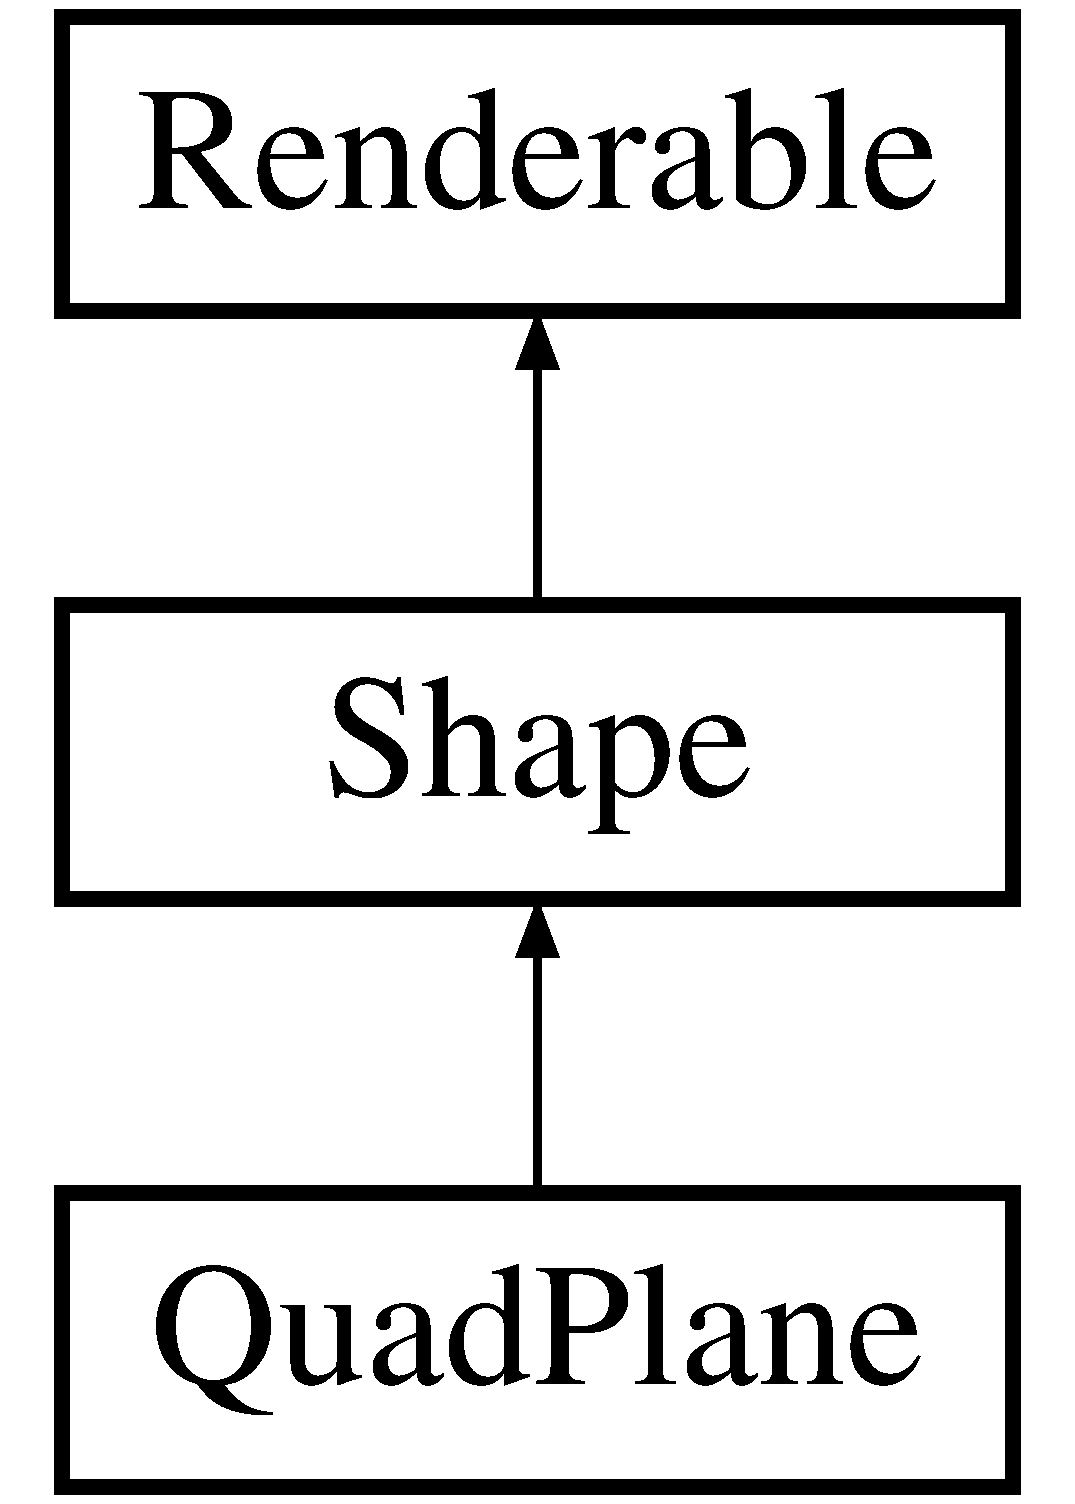
\includegraphics[height=3.000000cm]{class_quad_plane}
\end{center}
\end{figure}
\subsection*{Public Member Functions}
\begin{DoxyCompactItemize}
\item 
\hyperlink{class_quad_plane_ad5eaf38803814c882f5a458f4b0cc786}{Quad\-Plane} (const \hyperlink{class_vector3_d}{Vector3\-D} \&\hyperlink{class_quad_plane_af4e1dfc6a945fca065e6ab9387c05223}{normal}, float \hyperlink{class_quad_plane_aee2609c9c822afa7bc7397c190951bb5}{width}, float \hyperlink{class_quad_plane_a38aaa492e76f934ff0661e234ba6c19a}{depth})
\item 
\hyperlink{class_vector3_d}{Vector3\-D} \hyperlink{class_quad_plane_a1247c6efc9733e72da8b5ae09e560d78}{get\-Norm} () const 
\item 
float \hyperlink{class_quad_plane_a77004e91a9e7055234712629d0c3678d}{get\-Width} () const 
\item 
float \hyperlink{class_quad_plane_a5e5ebfcdad195a6a14e57669ac0a4c2e}{get\-Depth} () const 
\item 
const \hyperlink{class_quad_plane}{Quad\-Plane} \& \hyperlink{class_quad_plane_a385157caf428a4143c81440f9d2d0943}{convert} (const \hyperlink{class_shape}{Shape} \&s) const 
\end{DoxyCompactItemize}
\subsection*{Protected Attributes}
\begin{DoxyCompactItemize}
\item 
\hyperlink{class_vector3_d}{Vector3\-D} \hyperlink{class_quad_plane_af4e1dfc6a945fca065e6ab9387c05223}{normal}
\item 
float \hyperlink{class_quad_plane_aee2609c9c822afa7bc7397c190951bb5}{width}
\item 
float \hyperlink{class_quad_plane_a38aaa492e76f934ff0661e234ba6c19a}{depth}
\item 
float \hyperlink{class_quad_plane_a79fd779d6272282ea4879a9fedf8792c}{half\-Width}
\item 
float \hyperlink{class_quad_plane_a4b0a1e6811947b552b8a9227a8074e88}{half\-Depth}
\end{DoxyCompactItemize}
\subsection*{Additional Inherited Members}


\subsection{Constructor \& Destructor Documentation}
\hypertarget{class_quad_plane_ad5eaf38803814c882f5a458f4b0cc786}{\index{Quad\-Plane@{Quad\-Plane}!Quad\-Plane@{Quad\-Plane}}
\index{Quad\-Plane@{Quad\-Plane}!QuadPlane@{Quad\-Plane}}
\subsubsection[{Quad\-Plane}]{\setlength{\rightskip}{0pt plus 5cm}Quad\-Plane\-::\-Quad\-Plane (
\begin{DoxyParamCaption}
\item[{const {\bf Vector3\-D} \&}]{normal, }
\item[{float}]{width, }
\item[{float}]{depth}
\end{DoxyParamCaption}
)\hspace{0.3cm}{\ttfamily [inline]}}}\label{class_quad_plane_ad5eaf38803814c882f5a458f4b0cc786}


\subsection{Member Function Documentation}
\hypertarget{class_quad_plane_a385157caf428a4143c81440f9d2d0943}{\index{Quad\-Plane@{Quad\-Plane}!convert@{convert}}
\index{convert@{convert}!QuadPlane@{Quad\-Plane}}
\subsubsection[{convert}]{\setlength{\rightskip}{0pt plus 5cm}const {\bf Quad\-Plane}\& Quad\-Plane\-::convert (
\begin{DoxyParamCaption}
\item[{const {\bf Shape} \&}]{s}
\end{DoxyParamCaption}
) const\hspace{0.3cm}{\ttfamily [inline]}, {\ttfamily [virtual]}}}\label{class_quad_plane_a385157caf428a4143c81440f9d2d0943}


Implements \hyperlink{class_shape_ac07463606035fd9f8087a0673ca2c1a9}{Shape}.

\hypertarget{class_quad_plane_a5e5ebfcdad195a6a14e57669ac0a4c2e}{\index{Quad\-Plane@{Quad\-Plane}!get\-Depth@{get\-Depth}}
\index{get\-Depth@{get\-Depth}!QuadPlane@{Quad\-Plane}}
\subsubsection[{get\-Depth}]{\setlength{\rightskip}{0pt plus 5cm}float Quad\-Plane\-::get\-Depth (
\begin{DoxyParamCaption}
{}
\end{DoxyParamCaption}
) const\hspace{0.3cm}{\ttfamily [inline]}}}\label{class_quad_plane_a5e5ebfcdad195a6a14e57669ac0a4c2e}
\hypertarget{class_quad_plane_a1247c6efc9733e72da8b5ae09e560d78}{\index{Quad\-Plane@{Quad\-Plane}!get\-Norm@{get\-Norm}}
\index{get\-Norm@{get\-Norm}!QuadPlane@{Quad\-Plane}}
\subsubsection[{get\-Norm}]{\setlength{\rightskip}{0pt plus 5cm}{\bf Vector3\-D} Quad\-Plane\-::get\-Norm (
\begin{DoxyParamCaption}
{}
\end{DoxyParamCaption}
) const\hspace{0.3cm}{\ttfamily [inline]}}}\label{class_quad_plane_a1247c6efc9733e72da8b5ae09e560d78}
\hypertarget{class_quad_plane_a77004e91a9e7055234712629d0c3678d}{\index{Quad\-Plane@{Quad\-Plane}!get\-Width@{get\-Width}}
\index{get\-Width@{get\-Width}!QuadPlane@{Quad\-Plane}}
\subsubsection[{get\-Width}]{\setlength{\rightskip}{0pt plus 5cm}float Quad\-Plane\-::get\-Width (
\begin{DoxyParamCaption}
{}
\end{DoxyParamCaption}
) const\hspace{0.3cm}{\ttfamily [inline]}}}\label{class_quad_plane_a77004e91a9e7055234712629d0c3678d}


\subsection{Member Data Documentation}
\hypertarget{class_quad_plane_a38aaa492e76f934ff0661e234ba6c19a}{\index{Quad\-Plane@{Quad\-Plane}!depth@{depth}}
\index{depth@{depth}!QuadPlane@{Quad\-Plane}}
\subsubsection[{depth}]{\setlength{\rightskip}{0pt plus 5cm}float Quad\-Plane\-::depth\hspace{0.3cm}{\ttfamily [protected]}}}\label{class_quad_plane_a38aaa492e76f934ff0661e234ba6c19a}
\hypertarget{class_quad_plane_a4b0a1e6811947b552b8a9227a8074e88}{\index{Quad\-Plane@{Quad\-Plane}!half\-Depth@{half\-Depth}}
\index{half\-Depth@{half\-Depth}!QuadPlane@{Quad\-Plane}}
\subsubsection[{half\-Depth}]{\setlength{\rightskip}{0pt plus 5cm}float Quad\-Plane\-::half\-Depth\hspace{0.3cm}{\ttfamily [protected]}}}\label{class_quad_plane_a4b0a1e6811947b552b8a9227a8074e88}
\hypertarget{class_quad_plane_a79fd779d6272282ea4879a9fedf8792c}{\index{Quad\-Plane@{Quad\-Plane}!half\-Width@{half\-Width}}
\index{half\-Width@{half\-Width}!QuadPlane@{Quad\-Plane}}
\subsubsection[{half\-Width}]{\setlength{\rightskip}{0pt plus 5cm}float Quad\-Plane\-::half\-Width\hspace{0.3cm}{\ttfamily [protected]}}}\label{class_quad_plane_a79fd779d6272282ea4879a9fedf8792c}
\hypertarget{class_quad_plane_af4e1dfc6a945fca065e6ab9387c05223}{\index{Quad\-Plane@{Quad\-Plane}!normal@{normal}}
\index{normal@{normal}!QuadPlane@{Quad\-Plane}}
\subsubsection[{normal}]{\setlength{\rightskip}{0pt plus 5cm}{\bf Vector3\-D} Quad\-Plane\-::normal\hspace{0.3cm}{\ttfamily [protected]}}}\label{class_quad_plane_af4e1dfc6a945fca065e6ab9387c05223}
\hypertarget{class_quad_plane_aee2609c9c822afa7bc7397c190951bb5}{\index{Quad\-Plane@{Quad\-Plane}!width@{width}}
\index{width@{width}!QuadPlane@{Quad\-Plane}}
\subsubsection[{width}]{\setlength{\rightskip}{0pt plus 5cm}float Quad\-Plane\-::width\hspace{0.3cm}{\ttfamily [protected]}}}\label{class_quad_plane_aee2609c9c822afa7bc7397c190951bb5}


The documentation for this class was generated from the following file\-:\begin{DoxyCompactItemize}
\item 
D\-:/\-Development/\-My\-Projects/\-Physically\-Based\-Modeling/include/\hyperlink{_quad_plane_8h}{Quad\-Plane.\-h}\end{DoxyCompactItemize}

\hypertarget{class_r_b_deferred_force}{\section{R\-B\-Deferred\-Force Class Reference}
\label{class_r_b_deferred_force}\index{R\-B\-Deferred\-Force@{R\-B\-Deferred\-Force}}
}


{\ttfamily \#include $<$Rigid\-Body.\-h$>$}

Inheritance diagram for R\-B\-Deferred\-Force\-:\begin{figure}[H]
\begin{center}
\leavevmode
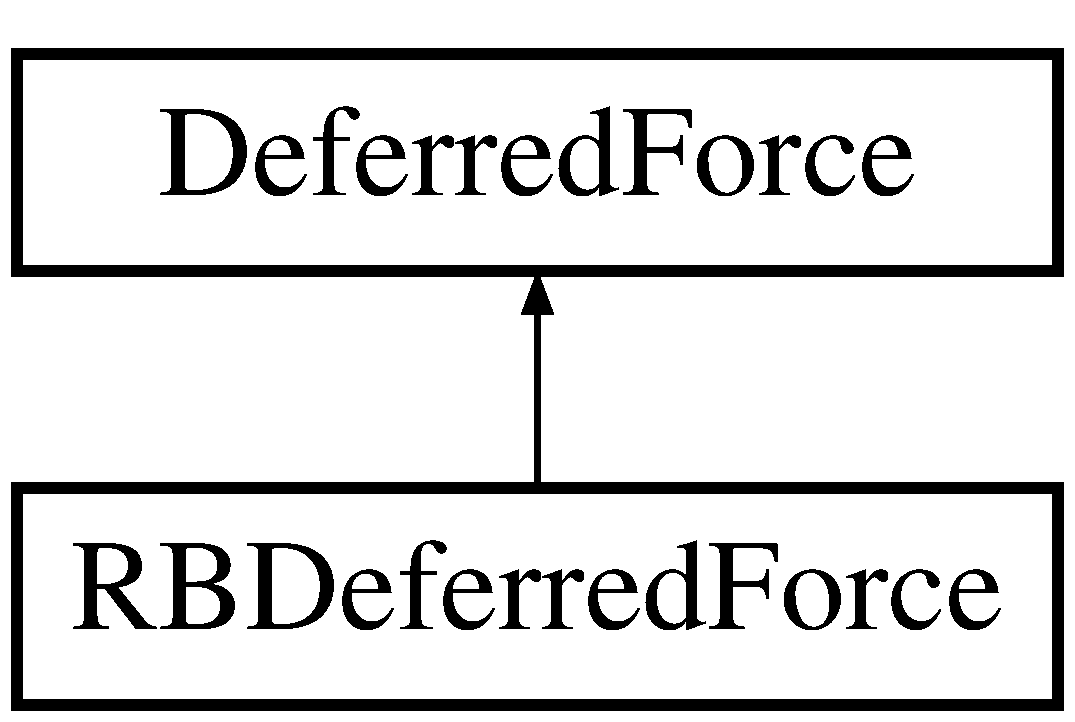
\includegraphics[height=2.000000cm]{class_r_b_deferred_force}
\end{center}
\end{figure}
\subsection*{Public Member Functions}
\begin{DoxyCompactItemize}
\item 
\hyperlink{class_r_b_deferred_force_a94a33b90bfbbbb35233b49fc032d3304}{R\-B\-Deferred\-Force} (const \hyperlink{class_vector3_d}{Vector3\-D} \&normal, float timestep\-Frac, const float \&mass0, const float \&friction0, const float \&elasticity0, const \hyperlink{class_vector3_d}{Vector3\-D} \&velocity0, const float \&mass1, const float \&friction1, const float \&elasticity1, const \hyperlink{class_vector3_d}{Vector3\-D} \&velocity1)
\item 
\hyperlink{class_force}{Force} $\ast$ \hyperlink{class_r_b_deferred_force_a35e7ec80d60e82e9175b06d864b0af2a}{get} (float \hyperlink{_physically_based_8h_ab9edcc09985767509bf717e25ac80ab7}{timestep})
\end{DoxyCompactItemize}
\subsection*{Additional Inherited Members}


\subsection{Constructor \& Destructor Documentation}
\hypertarget{class_r_b_deferred_force_a94a33b90bfbbbb35233b49fc032d3304}{\index{R\-B\-Deferred\-Force@{R\-B\-Deferred\-Force}!R\-B\-Deferred\-Force@{R\-B\-Deferred\-Force}}
\index{R\-B\-Deferred\-Force@{R\-B\-Deferred\-Force}!RBDeferredForce@{R\-B\-Deferred\-Force}}
\subsubsection[{R\-B\-Deferred\-Force}]{\setlength{\rightskip}{0pt plus 5cm}R\-B\-Deferred\-Force\-::\-R\-B\-Deferred\-Force (
\begin{DoxyParamCaption}
\item[{const {\bf Vector3\-D} \&}]{normal, }
\item[{float}]{timestep\-Frac, }
\item[{const float \&}]{mass0, }
\item[{const float \&}]{friction0, }
\item[{const float \&}]{elasticity0, }
\item[{const {\bf Vector3\-D} \&}]{velocity0, }
\item[{const float \&}]{mass1, }
\item[{const float \&}]{friction1, }
\item[{const float \&}]{elasticity1, }
\item[{const {\bf Vector3\-D} \&}]{velocity1}
\end{DoxyParamCaption}
)\hspace{0.3cm}{\ttfamily [inline]}}}\label{class_r_b_deferred_force_a94a33b90bfbbbb35233b49fc032d3304}


\subsection{Member Function Documentation}
\hypertarget{class_r_b_deferred_force_a35e7ec80d60e82e9175b06d864b0af2a}{\index{R\-B\-Deferred\-Force@{R\-B\-Deferred\-Force}!get@{get}}
\index{get@{get}!RBDeferredForce@{R\-B\-Deferred\-Force}}
\subsubsection[{get}]{\setlength{\rightskip}{0pt plus 5cm}{\bf Force}$\ast$ R\-B\-Deferred\-Force\-::get (
\begin{DoxyParamCaption}
\item[{float}]{timestep}
\end{DoxyParamCaption}
)\hspace{0.3cm}{\ttfamily [inline]}}}\label{class_r_b_deferred_force_a35e7ec80d60e82e9175b06d864b0af2a}


The documentation for this class was generated from the following file\-:\begin{DoxyCompactItemize}
\item 
D\-:/\-Development/\-My\-Projects/\-Physically\-Based\-Modeling/include/\hyperlink{_rigid_body_8h}{Rigid\-Body.\-h}\end{DoxyCompactItemize}

\hypertarget{class_renderable}{\section{Renderable Class Reference}
\label{class_renderable}\index{Renderable@{Renderable}}
}


{\ttfamily \#include $<$Renderable.\-h$>$}

Inheritance diagram for Renderable\-:\begin{figure}[H]
\begin{center}
\leavevmode
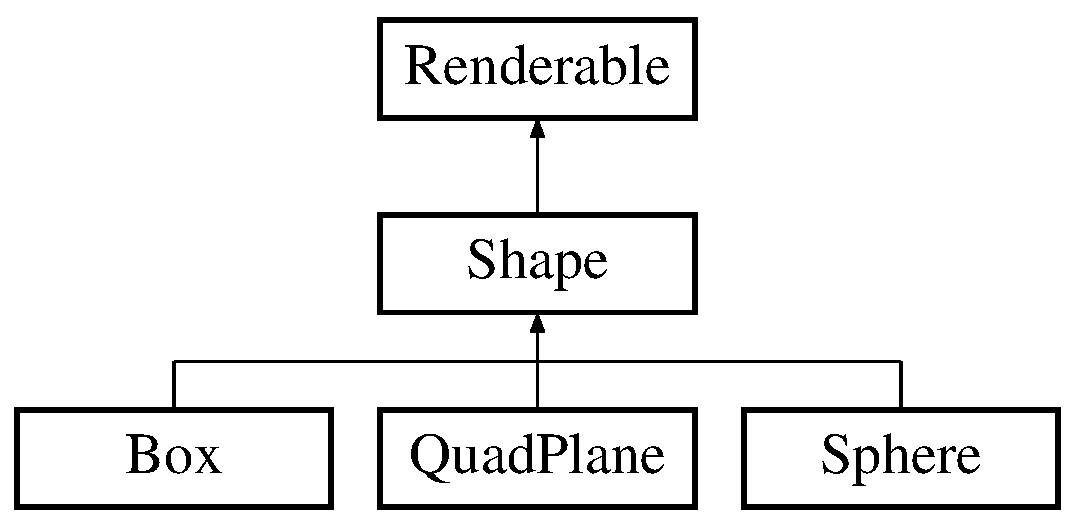
\includegraphics[height=3.000000cm]{class_renderable}
\end{center}
\end{figure}
\subsection*{Public Member Functions}
\begin{DoxyCompactItemize}
\item 
\hyperlink{class_renderable_a97a0f6efd2a058dfb003e64e63bdb255}{Renderable} ()
\item 
virtual void \hyperlink{class_renderable_af8e5354d0e109e8421d4a23035449204}{open\-G\-L\-Draw} () const =0
\end{DoxyCompactItemize}


\subsection{Constructor \& Destructor Documentation}
\hypertarget{class_renderable_a97a0f6efd2a058dfb003e64e63bdb255}{\index{Renderable@{Renderable}!Renderable@{Renderable}}
\index{Renderable@{Renderable}!Renderable@{Renderable}}
\subsubsection[{Renderable}]{\setlength{\rightskip}{0pt plus 5cm}Renderable\-::\-Renderable (
\begin{DoxyParamCaption}
{}
\end{DoxyParamCaption}
)\hspace{0.3cm}{\ttfamily [inline]}}}\label{class_renderable_a97a0f6efd2a058dfb003e64e63bdb255}


\subsection{Member Function Documentation}
\hypertarget{class_renderable_af8e5354d0e109e8421d4a23035449204}{\index{Renderable@{Renderable}!open\-G\-L\-Draw@{open\-G\-L\-Draw}}
\index{open\-G\-L\-Draw@{open\-G\-L\-Draw}!Renderable@{Renderable}}
\subsubsection[{open\-G\-L\-Draw}]{\setlength{\rightskip}{0pt plus 5cm}virtual void Renderable\-::open\-G\-L\-Draw (
\begin{DoxyParamCaption}
{}
\end{DoxyParamCaption}
) const\hspace{0.3cm}{\ttfamily [pure virtual]}}}\label{class_renderable_af8e5354d0e109e8421d4a23035449204}


The documentation for this class was generated from the following file\-:\begin{DoxyCompactItemize}
\item 
D\-:/\-Development/\-My\-Projects/\-Physically\-Based\-Modeling/include/\hyperlink{_renderable_8h}{Renderable.\-h}\end{DoxyCompactItemize}

\hypertarget{class_rigid_body}{\section{Rigid\-Body Class Reference}
\label{class_rigid_body}\index{Rigid\-Body@{Rigid\-Body}}
}


{\ttfamily \#include $<$Rigid\-Body.\-h$>$}

Inheritance diagram for Rigid\-Body\-:\begin{figure}[H]
\begin{center}
\leavevmode
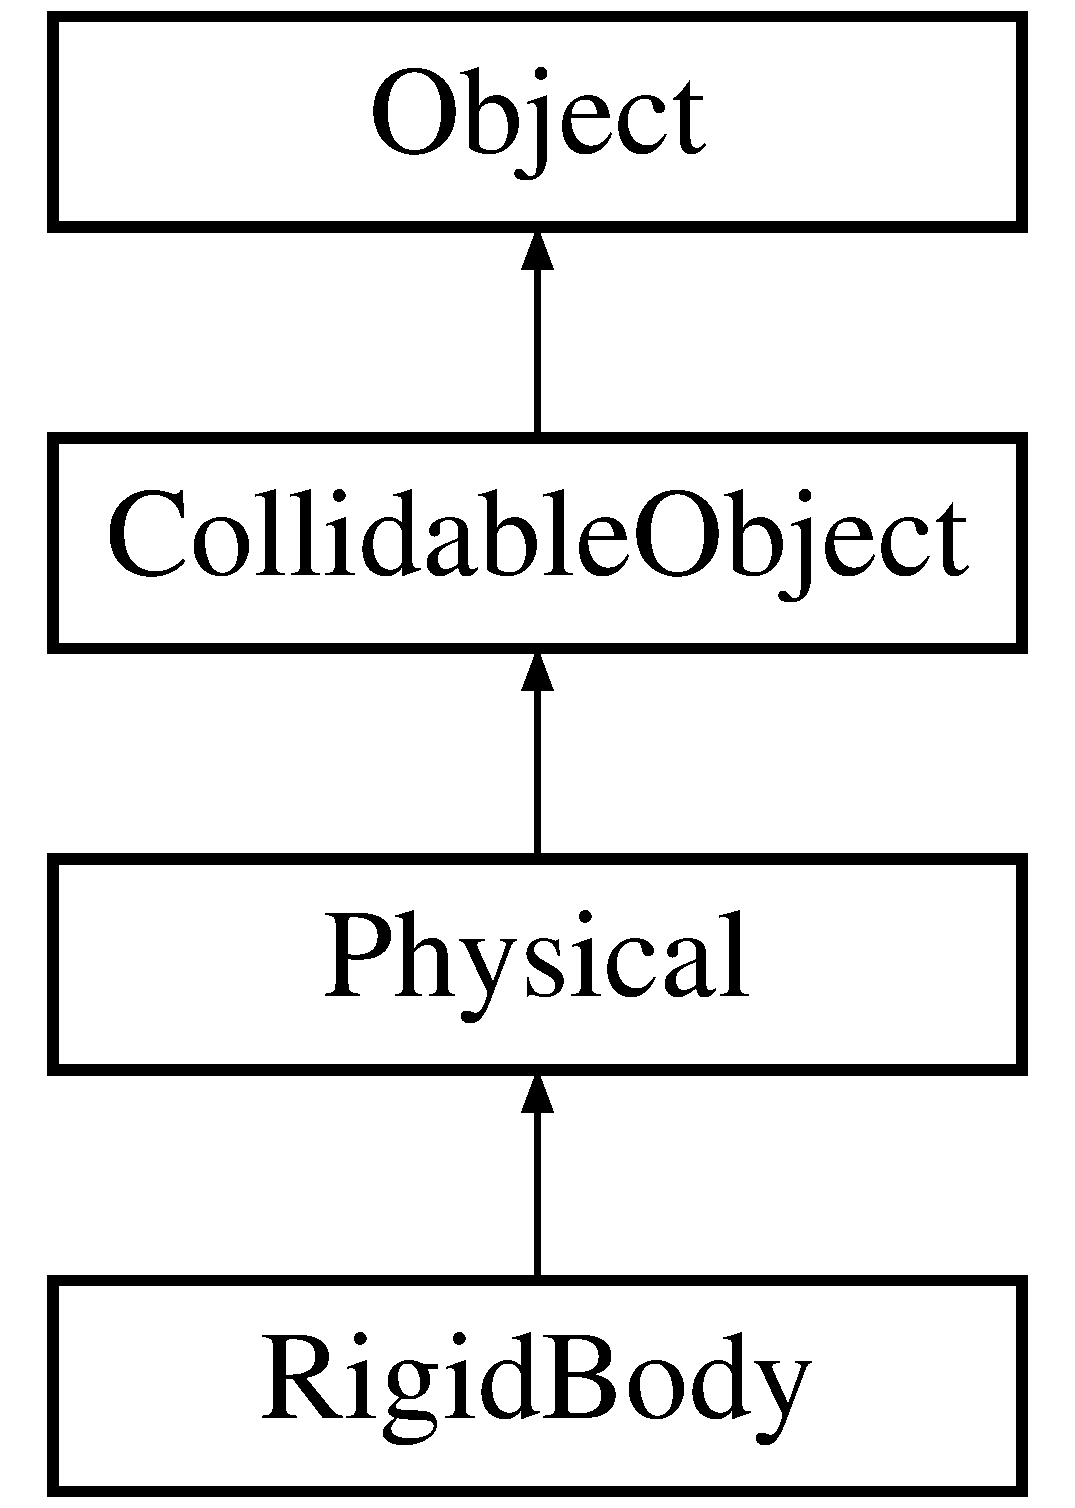
\includegraphics[height=4.000000cm]{class_rigid_body}
\end{center}
\end{figure}
\subsection*{Public Member Functions}
\begin{DoxyCompactItemize}
\item 
\hyperlink{class_rigid_body_ac47fcf37b361af982da6ec3ecd799607}{Rigid\-Body} (float mass, const \hyperlink{class_vector3_d}{Vector3\-D} \&cog, float fric, float elasticity, const \hyperlink{class_vector3_d}{Vector3\-D} \&velocity)
\item 
virtual \hyperlink{class_deferred_force}{Deferred\-Force} $\ast$ \hyperlink{class_rigid_body_a4b18eaaeb72f18c9f7d3f060d357e974}{get\-Collision\-Force} (const \hyperlink{class_collidable_object}{Collidable\-Object} \&co, const \hyperlink{class_vector3_d}{Vector3\-D} \&normal)
\end{DoxyCompactItemize}
\subsection*{Additional Inherited Members}


\subsection{Constructor \& Destructor Documentation}
\hypertarget{class_rigid_body_ac47fcf37b361af982da6ec3ecd799607}{\index{Rigid\-Body@{Rigid\-Body}!Rigid\-Body@{Rigid\-Body}}
\index{Rigid\-Body@{Rigid\-Body}!RigidBody@{Rigid\-Body}}
\subsubsection[{Rigid\-Body}]{\setlength{\rightskip}{0pt plus 5cm}Rigid\-Body\-::\-Rigid\-Body (
\begin{DoxyParamCaption}
\item[{float}]{mass, }
\item[{const {\bf Vector3\-D} \&}]{cog, }
\item[{float}]{fric, }
\item[{float}]{elasticity, }
\item[{const {\bf Vector3\-D} \&}]{velocity}
\end{DoxyParamCaption}
)}}\label{class_rigid_body_ac47fcf37b361af982da6ec3ecd799607}


\subsection{Member Function Documentation}
\hypertarget{class_rigid_body_a4b18eaaeb72f18c9f7d3f060d357e974}{\index{Rigid\-Body@{Rigid\-Body}!get\-Collision\-Force@{get\-Collision\-Force}}
\index{get\-Collision\-Force@{get\-Collision\-Force}!RigidBody@{Rigid\-Body}}
\subsubsection[{get\-Collision\-Force}]{\setlength{\rightskip}{0pt plus 5cm}virtual {\bf Deferred\-Force}$\ast$ Rigid\-Body\-::get\-Collision\-Force (
\begin{DoxyParamCaption}
\item[{const {\bf Collidable\-Object} \&}]{co, }
\item[{const {\bf Vector3\-D} \&}]{normal}
\end{DoxyParamCaption}
)\hspace{0.3cm}{\ttfamily [inline]}, {\ttfamily [virtual]}}}\label{class_rigid_body_a4b18eaaeb72f18c9f7d3f060d357e974}


Implements \hyperlink{class_collidable_object_ad1ad2104aa96351a206ffe6540d84090}{Collidable\-Object}.



The documentation for this class was generated from the following file\-:\begin{DoxyCompactItemize}
\item 
D\-:/\-Development/\-My\-Projects/\-Physically\-Based\-Modeling/include/\hyperlink{_rigid_body_8h}{Rigid\-Body.\-h}\end{DoxyCompactItemize}

\hypertarget{class_r_w_wrapper}{\section{R\-W\-Wrapper Class Reference}
\label{class_r_w_wrapper}\index{R\-W\-Wrapper@{R\-W\-Wrapper}}
}


{\ttfamily \#include $<$render\-Window\-Wrapper.\-h$>$}

Inheritance diagram for R\-W\-Wrapper\-:\begin{figure}[H]
\begin{center}
\leavevmode
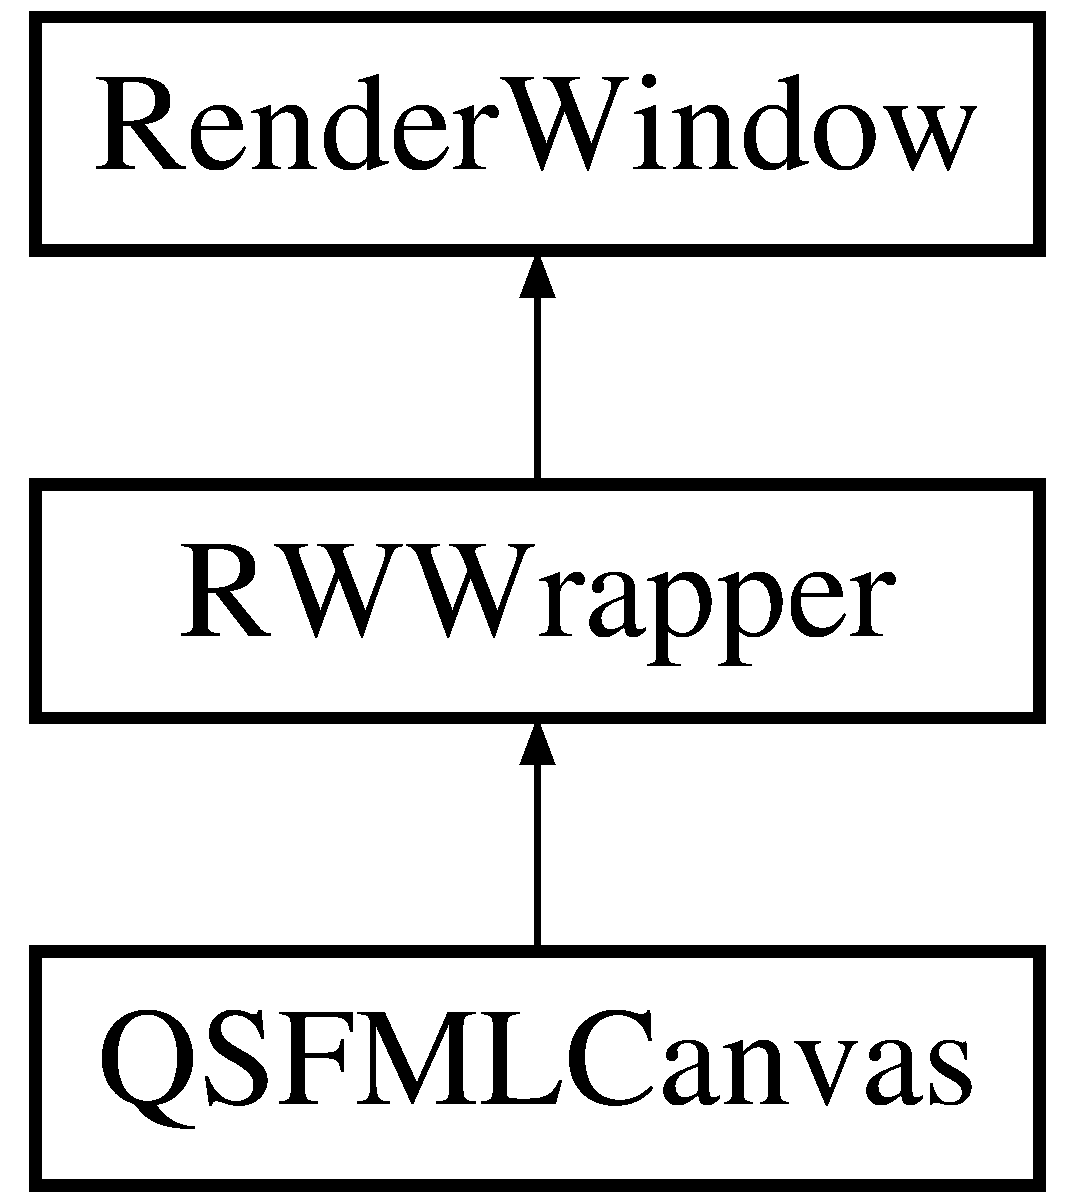
\includegraphics[height=3.000000cm]{class_r_w_wrapper}
\end{center}
\end{figure}
\subsection*{Public Member Functions}
\begin{DoxyCompactItemize}
\item 
void \hyperlink{class_r_w_wrapper_a48816a6939359dc800bc3e2c1bf492c9}{create\-Render\-Window} (sf\-::\-Window\-Handle wh)
\end{DoxyCompactItemize}


\subsection{Member Function Documentation}
\hypertarget{class_r_w_wrapper_a48816a6939359dc800bc3e2c1bf492c9}{\index{R\-W\-Wrapper@{R\-W\-Wrapper}!create\-Render\-Window@{create\-Render\-Window}}
\index{create\-Render\-Window@{create\-Render\-Window}!RWWrapper@{R\-W\-Wrapper}}
\subsubsection[{create\-Render\-Window}]{\setlength{\rightskip}{0pt plus 5cm}void R\-W\-Wrapper\-::create\-Render\-Window (
\begin{DoxyParamCaption}
\item[{sf\-::\-Window\-Handle}]{wh}
\end{DoxyParamCaption}
)\hspace{0.3cm}{\ttfamily [inline]}}}\label{class_r_w_wrapper_a48816a6939359dc800bc3e2c1bf492c9}


The documentation for this class was generated from the following file\-:\begin{DoxyCompactItemize}
\item 
D\-:/\-Development/\-My\-Projects/\-Physically\-Based\-Modeling/include/\-G\-U\-I/\hyperlink{render_window_wrapper_8h}{render\-Window\-Wrapper.\-h}\end{DoxyCompactItemize}

\hypertarget{class_shape}{\section{Shape Class Reference}
\label{class_shape}\index{Shape@{Shape}}
}


{\ttfamily \#include $<$Shape.\-h$>$}

Inheritance diagram for Shape\-:\begin{figure}[H]
\begin{center}
\leavevmode
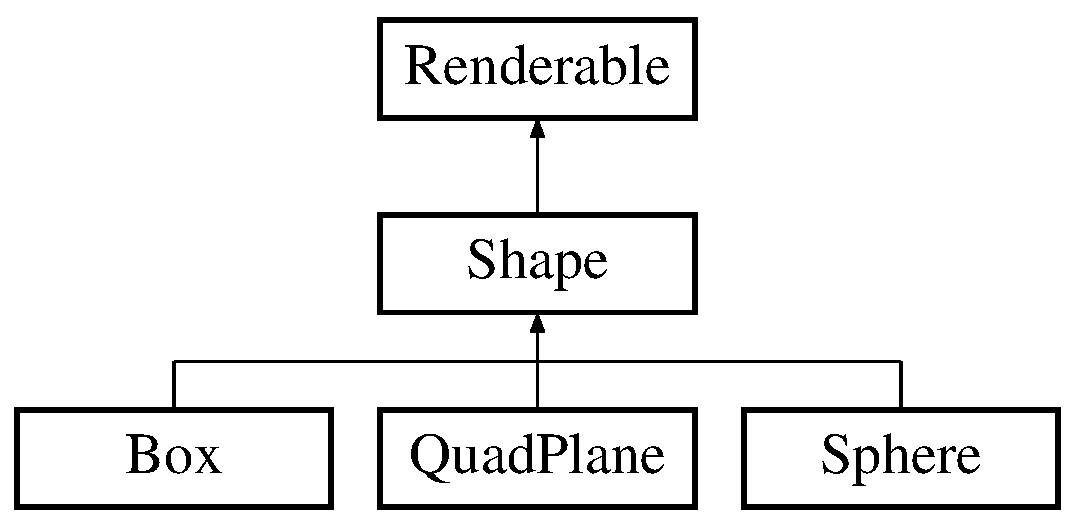
\includegraphics[height=3.000000cm]{class_shape}
\end{center}
\end{figure}
\subsection*{Public Member Functions}
\begin{DoxyCompactItemize}
\item 
virtual \hyperlink{class_shape_ac3b9fc48965274893f25b18aa14ba665}{$\sim$\-Shape} ()
\item 
virtual bool \hyperlink{class_shape_af62169dcec74b96697f74d9740d03caa}{collision} (const \hyperlink{class_shape}{Shape} \&this\-Updated, const \hyperlink{class_shape}{Shape} \&other, const \hyperlink{class_shape}{Shape} \&other\-Updated, float \&timestep\-Frac, \hyperlink{class_vector3_d}{Vector3\-D} \&collision\-Normal)
\item 
$<$ typename\-T $>$ virtual bool \hyperlink{class_shape_a4f36cc75a8ee27039ec783d4e3fe40f5}{collide\-With} (const \hyperlink{class_shape}{Shape} \&this\-Updated, const T \&other, const T \&other\-Updated, float \&timestep\-Frac, \hyperlink{class_vector3_d}{Vector3\-D} \&collision\-Normal)
\item 
virtual const \hyperlink{class_shape}{Shape} \& \hyperlink{class_shape_ac07463606035fd9f8087a0673ca2c1a9}{convert} (const \hyperlink{class_shape}{Shape} \&s) const =0
\item 
friend$<$ typename T1, typename \\*
T2 $>$ bool \hyperlink{class_shape_ae8db86e01fff600eb320502d2f9f49e9}{Collision\-Handler\-::collision} (const T1 \&s1, const T1 \&s1\-\_\-potential, const T2 \&s2, const T2 \&s2\-\_\-potential, float \&timestep\-Frac, \hyperlink{class_collision_force}{Collision\-Force} \&collision\-Force)
\end{DoxyCompactItemize}
\subsection*{Public Attributes}
\begin{DoxyCompactItemize}
\item 
\hyperlink{class_transform}{Transform} \hyperlink{class_shape_aedca08a4f2ac7f744160bbb62ec399df}{transform}
\end{DoxyCompactItemize}
\subsection*{Protected Member Functions}
\begin{DoxyCompactItemize}
\item 
\hyperlink{class_shape_aaa8d87171e65e0d8ba3c5459978992a7}{Shape} ()
\end{DoxyCompactItemize}


\subsection{Constructor \& Destructor Documentation}
\hypertarget{class_shape_ac3b9fc48965274893f25b18aa14ba665}{\index{Shape@{Shape}!$\sim$\-Shape@{$\sim$\-Shape}}
\index{$\sim$\-Shape@{$\sim$\-Shape}!Shape@{Shape}}
\subsubsection[{$\sim$\-Shape}]{\setlength{\rightskip}{0pt plus 5cm}virtual Shape\-::$\sim$\-Shape (
\begin{DoxyParamCaption}
{}
\end{DoxyParamCaption}
)\hspace{0.3cm}{\ttfamily [inline]}, {\ttfamily [virtual]}}}\label{class_shape_ac3b9fc48965274893f25b18aa14ba665}
\hypertarget{class_shape_aaa8d87171e65e0d8ba3c5459978992a7}{\index{Shape@{Shape}!Shape@{Shape}}
\index{Shape@{Shape}!Shape@{Shape}}
\subsubsection[{Shape}]{\setlength{\rightskip}{0pt plus 5cm}Shape\-::\-Shape (
\begin{DoxyParamCaption}
{}
\end{DoxyParamCaption}
)\hspace{0.3cm}{\ttfamily [inline]}, {\ttfamily [protected]}}}\label{class_shape_aaa8d87171e65e0d8ba3c5459978992a7}


\subsection{Member Function Documentation}
\hypertarget{class_shape_a4f36cc75a8ee27039ec783d4e3fe40f5}{\index{Shape@{Shape}!collide\-With@{collide\-With}}
\index{collide\-With@{collide\-With}!Shape@{Shape}}
\subsubsection[{collide\-With}]{\setlength{\rightskip}{0pt plus 5cm}$<$typename\-T$>$ virtual bool Shape\-::collide\-With (
\begin{DoxyParamCaption}
\item[{const {\bf Shape} \&}]{this\-Updated, }
\item[{const T \&}]{other, }
\item[{const T \&}]{other\-Updated, }
\item[{float \&}]{timestep\-Frac, }
\item[{{\bf Vector3\-D} \&}]{collision\-Normal}
\end{DoxyParamCaption}
)\hspace{0.3cm}{\ttfamily [inline]}, {\ttfamily [virtual]}}}\label{class_shape_a4f36cc75a8ee27039ec783d4e3fe40f5}
\hypertarget{class_shape_af62169dcec74b96697f74d9740d03caa}{\index{Shape@{Shape}!collision@{collision}}
\index{collision@{collision}!Shape@{Shape}}
\subsubsection[{collision}]{\setlength{\rightskip}{0pt plus 5cm}virtual bool Shape\-::collision (
\begin{DoxyParamCaption}
\item[{const {\bf Shape} \&}]{this\-Updated, }
\item[{const {\bf Shape} \&}]{other, }
\item[{const {\bf Shape} \&}]{other\-Updated, }
\item[{float \&}]{timestep\-Frac, }
\item[{{\bf Vector3\-D} \&}]{collision\-Normal}
\end{DoxyParamCaption}
)\hspace{0.3cm}{\ttfamily [inline]}, {\ttfamily [virtual]}}}\label{class_shape_af62169dcec74b96697f74d9740d03caa}
\hypertarget{class_shape_ae8db86e01fff600eb320502d2f9f49e9}{\index{Shape@{Shape}!Collision\-Handler\-::collision@{Collision\-Handler\-::collision}}
\index{Collision\-Handler\-::collision@{Collision\-Handler\-::collision}!Shape@{Shape}}
\subsubsection[{Collision\-Handler\-::collision}]{\setlength{\rightskip}{0pt plus 5cm}friend$<$typename T1, typename T2$>$ bool Shape\-::\-Collision\-Handler\-::collision (
\begin{DoxyParamCaption}
\item[{const T1 \&}]{s1, }
\item[{const T1 \&}]{s1\-\_\-potential, }
\item[{const T2 \&}]{s2, }
\item[{const T2 \&}]{s2\-\_\-potential, }
\item[{float \&}]{timestep\-Frac, }
\item[{{\bf Collision\-Force} \&}]{collision\-Force}
\end{DoxyParamCaption}
)}}\label{class_shape_ae8db86e01fff600eb320502d2f9f49e9}
\hypertarget{class_shape_ac07463606035fd9f8087a0673ca2c1a9}{\index{Shape@{Shape}!convert@{convert}}
\index{convert@{convert}!Shape@{Shape}}
\subsubsection[{convert}]{\setlength{\rightskip}{0pt plus 5cm}virtual const {\bf Shape}\& Shape\-::convert (
\begin{DoxyParamCaption}
\item[{const {\bf Shape} \&}]{s}
\end{DoxyParamCaption}
) const\hspace{0.3cm}{\ttfamily [pure virtual]}}}\label{class_shape_ac07463606035fd9f8087a0673ca2c1a9}


Implemented in \hyperlink{class_quad_plane_a385157caf428a4143c81440f9d2d0943}{Quad\-Plane}, and \hyperlink{class_sphere_a6c20d328c6b2d1788d329e8bb3c7d070}{Sphere}.



\subsection{Member Data Documentation}
\hypertarget{class_shape_aedca08a4f2ac7f744160bbb62ec399df}{\index{Shape@{Shape}!transform@{transform}}
\index{transform@{transform}!Shape@{Shape}}
\subsubsection[{transform}]{\setlength{\rightskip}{0pt plus 5cm}{\bf Transform} Shape\-::transform}}\label{class_shape_aedca08a4f2ac7f744160bbb62ec399df}


The documentation for this class was generated from the following file\-:\begin{DoxyCompactItemize}
\item 
D\-:/\-Development/\-My\-Projects/\-Physically\-Based\-Modeling/include/\hyperlink{_shape_8h}{Shape.\-h}\end{DoxyCompactItemize}

\hypertarget{class_simple_deferred_force}{\section{Simple\-Deferred\-Force Class Reference}
\label{class_simple_deferred_force}\index{Simple\-Deferred\-Force@{Simple\-Deferred\-Force}}
}


{\ttfamily \#include $<$Collider\-Object.\-h$>$}

Inheritance diagram for Simple\-Deferred\-Force\-:\begin{figure}[H]
\begin{center}
\leavevmode
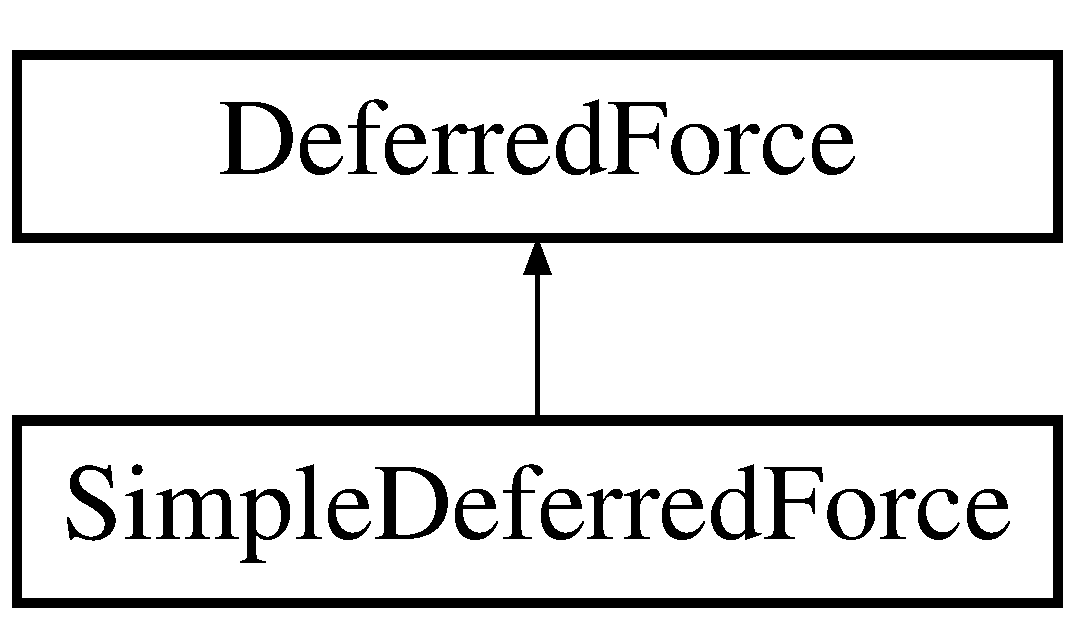
\includegraphics[height=2.000000cm]{class_simple_deferred_force}
\end{center}
\end{figure}
\subsection*{Public Member Functions}
\begin{DoxyCompactItemize}
\item 
\hyperlink{class_simple_deferred_force_abade91bffd4e1e87ecff47ada68ff271}{Simple\-Deferred\-Force} (const \hyperlink{class_vector3_d}{Vector3\-D} \&normal)
\item 
\hyperlink{class_force}{Force} $\ast$ \hyperlink{class_simple_deferred_force_a2b37ad69d9c6969149bea8868db4ee6a}{get} (float \hyperlink{_physically_based_8h_ab9edcc09985767509bf717e25ac80ab7}{timestep})
\end{DoxyCompactItemize}
\subsection*{Additional Inherited Members}


\subsection{Constructor \& Destructor Documentation}
\hypertarget{class_simple_deferred_force_abade91bffd4e1e87ecff47ada68ff271}{\index{Simple\-Deferred\-Force@{Simple\-Deferred\-Force}!Simple\-Deferred\-Force@{Simple\-Deferred\-Force}}
\index{Simple\-Deferred\-Force@{Simple\-Deferred\-Force}!SimpleDeferredForce@{Simple\-Deferred\-Force}}
\subsubsection[{Simple\-Deferred\-Force}]{\setlength{\rightskip}{0pt plus 5cm}Simple\-Deferred\-Force\-::\-Simple\-Deferred\-Force (
\begin{DoxyParamCaption}
\item[{const {\bf Vector3\-D} \&}]{normal}
\end{DoxyParamCaption}
)\hspace{0.3cm}{\ttfamily [inline]}}}\label{class_simple_deferred_force_abade91bffd4e1e87ecff47ada68ff271}


\subsection{Member Function Documentation}
\hypertarget{class_simple_deferred_force_a2b37ad69d9c6969149bea8868db4ee6a}{\index{Simple\-Deferred\-Force@{Simple\-Deferred\-Force}!get@{get}}
\index{get@{get}!SimpleDeferredForce@{Simple\-Deferred\-Force}}
\subsubsection[{get}]{\setlength{\rightskip}{0pt plus 5cm}{\bf Force}$\ast$ Simple\-Deferred\-Force\-::get (
\begin{DoxyParamCaption}
\item[{float}]{timestep}
\end{DoxyParamCaption}
)\hspace{0.3cm}{\ttfamily [inline]}}}\label{class_simple_deferred_force_a2b37ad69d9c6969149bea8868db4ee6a}


The documentation for this class was generated from the following file\-:\begin{DoxyCompactItemize}
\item 
D\-:/\-Development/\-My\-Projects/\-Physically\-Based\-Modeling/include/\hyperlink{_collider_object_8h}{Collider\-Object.\-h}\end{DoxyCompactItemize}

\hypertarget{class_sphere}{\section{Sphere Class Reference}
\label{class_sphere}\index{Sphere@{Sphere}}
}


{\ttfamily \#include $<$Sphere.\-h$>$}

Inheritance diagram for Sphere\-:\begin{figure}[H]
\begin{center}
\leavevmode
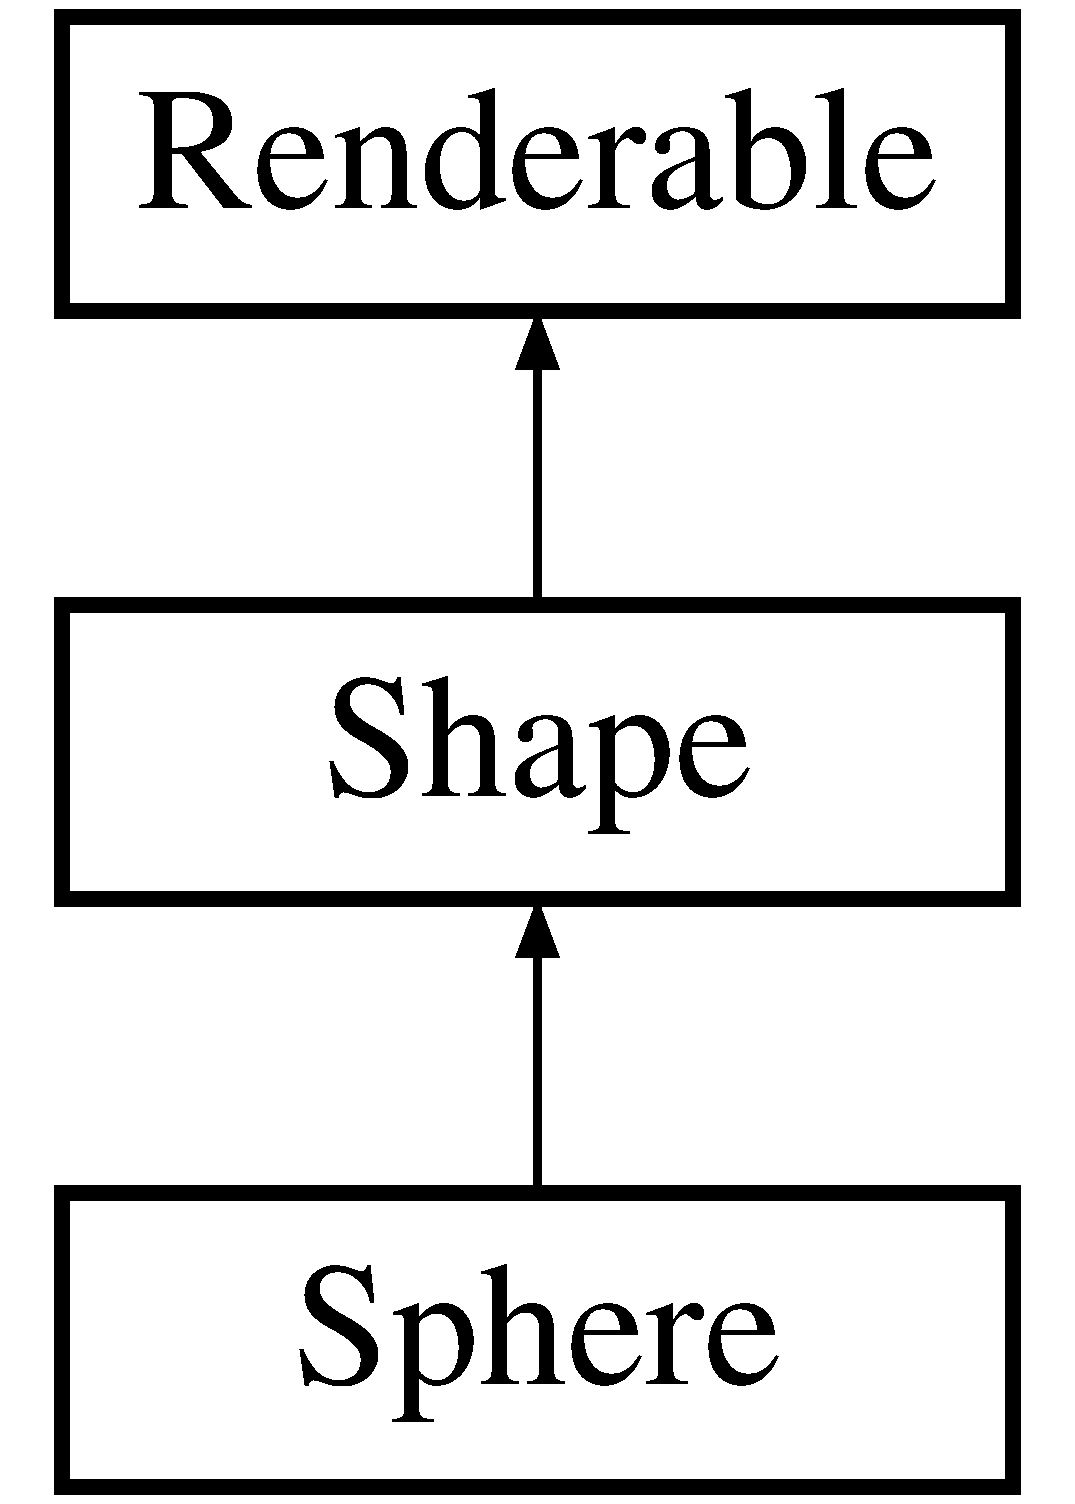
\includegraphics[height=3.000000cm]{class_sphere}
\end{center}
\end{figure}
\subsection*{Public Member Functions}
\begin{DoxyCompactItemize}
\item 
\hyperlink{class_sphere_ab6324c968f5db50b7ea4d5c3fa94aab2}{Sphere} (float r)
\item 
float \hyperlink{class_sphere_a50eef09c3020fe3ed0df7b285d0c917f}{get\-Rad} () const 
\item 
const \hyperlink{class_sphere}{Sphere} \& \hyperlink{class_sphere_a6c20d328c6b2d1788d329e8bb3c7d070}{convert} (const \hyperlink{class_shape}{Shape} \&s) const 
\end{DoxyCompactItemize}
\subsection*{Protected Attributes}
\begin{DoxyCompactItemize}
\item 
float \hyperlink{class_sphere_ae6f42f0da6679a2f0b4a22681ccccf38}{radius}
\item 
double \hyperlink{class_sphere_a1619b936ab9aeadccc881a9117a336a4}{radius\-Sq}
\end{DoxyCompactItemize}
\subsection*{Additional Inherited Members}


\subsection{Constructor \& Destructor Documentation}
\hypertarget{class_sphere_ab6324c968f5db50b7ea4d5c3fa94aab2}{\index{Sphere@{Sphere}!Sphere@{Sphere}}
\index{Sphere@{Sphere}!Sphere@{Sphere}}
\subsubsection[{Sphere}]{\setlength{\rightskip}{0pt plus 5cm}Sphere\-::\-Sphere (
\begin{DoxyParamCaption}
\item[{float}]{r}
\end{DoxyParamCaption}
)\hspace{0.3cm}{\ttfamily [inline]}}}\label{class_sphere_ab6324c968f5db50b7ea4d5c3fa94aab2}


\subsection{Member Function Documentation}
\hypertarget{class_sphere_a6c20d328c6b2d1788d329e8bb3c7d070}{\index{Sphere@{Sphere}!convert@{convert}}
\index{convert@{convert}!Sphere@{Sphere}}
\subsubsection[{convert}]{\setlength{\rightskip}{0pt plus 5cm}const {\bf Sphere}\& Sphere\-::convert (
\begin{DoxyParamCaption}
\item[{const {\bf Shape} \&}]{s}
\end{DoxyParamCaption}
) const\hspace{0.3cm}{\ttfamily [inline]}, {\ttfamily [virtual]}}}\label{class_sphere_a6c20d328c6b2d1788d329e8bb3c7d070}


Implements \hyperlink{class_shape_ac07463606035fd9f8087a0673ca2c1a9}{Shape}.

\hypertarget{class_sphere_a50eef09c3020fe3ed0df7b285d0c917f}{\index{Sphere@{Sphere}!get\-Rad@{get\-Rad}}
\index{get\-Rad@{get\-Rad}!Sphere@{Sphere}}
\subsubsection[{get\-Rad}]{\setlength{\rightskip}{0pt plus 5cm}float Sphere\-::get\-Rad (
\begin{DoxyParamCaption}
{}
\end{DoxyParamCaption}
) const\hspace{0.3cm}{\ttfamily [inline]}}}\label{class_sphere_a50eef09c3020fe3ed0df7b285d0c917f}


\subsection{Member Data Documentation}
\hypertarget{class_sphere_ae6f42f0da6679a2f0b4a22681ccccf38}{\index{Sphere@{Sphere}!radius@{radius}}
\index{radius@{radius}!Sphere@{Sphere}}
\subsubsection[{radius}]{\setlength{\rightskip}{0pt plus 5cm}float Sphere\-::radius\hspace{0.3cm}{\ttfamily [protected]}}}\label{class_sphere_ae6f42f0da6679a2f0b4a22681ccccf38}
\hypertarget{class_sphere_a1619b936ab9aeadccc881a9117a336a4}{\index{Sphere@{Sphere}!radius\-Sq@{radius\-Sq}}
\index{radius\-Sq@{radius\-Sq}!Sphere@{Sphere}}
\subsubsection[{radius\-Sq}]{\setlength{\rightskip}{0pt plus 5cm}double Sphere\-::radius\-Sq\hspace{0.3cm}{\ttfamily [protected]}}}\label{class_sphere_a1619b936ab9aeadccc881a9117a336a4}


The documentation for this class was generated from the following file\-:\begin{DoxyCompactItemize}
\item 
D\-:/\-Development/\-My\-Projects/\-Physically\-Based\-Modeling/include/\hyperlink{_sphere_8h}{Sphere.\-h}\end{DoxyCompactItemize}

\hypertarget{class_transform}{\section{Transform Class Reference}
\label{class_transform}\index{Transform@{Transform}}
}


{\ttfamily \#include $<$Transform.\-h$>$}

\subsection*{Public Member Functions}
\begin{DoxyCompactItemize}
\item 
\hyperlink{class_transform_aa08ca4266efabc768973cdeea51945ab}{Transform} ()
\item 
\hyperlink{class_transform_a061a1a8e9dda0aaca268d2c5a86ba52e}{Transform} (const \hyperlink{class_matrix3_d}{Matrix3\-D} \&m)
\item 
\hyperlink{class_vector3_d}{Vector3\-D} \hyperlink{class_transform_a6bf31a150ad92d2526421081a301a668}{get\-Pos} () const 
\item 
\hyperlink{class_transform}{Transform} \hyperlink{class_transform_aeb37ee8512f05688c4aa6efbd36dd6b6}{transform\-Other} (const \hyperlink{class_transform}{Transform} \&t)
\item 
\hyperlink{class_transform}{Transform} \hyperlink{class_transform_a9c305c77f1dca3418b47dd1c1545a9fe}{transform\-Child} (const \hyperlink{class_transform}{Transform} \&t)
\item 
void \hyperlink{class_transform_a57a76ef2d274c5c8632e98fccca0f487}{translate} (double x, double y, double z)
\item 
void \hyperlink{class_transform_a2000fcffdb02984c2c5e51da4ff2afa0}{rotate} (double x, double y, double z)
\item 
void \hyperlink{class_transform_a9b3b1b60a8c4589d049e1e5fa62db4aa}{scale} (double x, double y, double z)
\item 
void \hyperlink{class_transform_acb521d818273c06fe88e306c8076e557}{apply\-Transform} (const \hyperlink{class_transform}{Transform} \&t)
\end{DoxyCompactItemize}


\subsection{Constructor \& Destructor Documentation}
\hypertarget{class_transform_aa08ca4266efabc768973cdeea51945ab}{\index{Transform@{Transform}!Transform@{Transform}}
\index{Transform@{Transform}!Transform@{Transform}}
\subsubsection[{Transform}]{\setlength{\rightskip}{0pt plus 5cm}Transform\-::\-Transform (
\begin{DoxyParamCaption}
{}
\end{DoxyParamCaption}
)\hspace{0.3cm}{\ttfamily [inline]}}}\label{class_transform_aa08ca4266efabc768973cdeea51945ab}
\hypertarget{class_transform_a061a1a8e9dda0aaca268d2c5a86ba52e}{\index{Transform@{Transform}!Transform@{Transform}}
\index{Transform@{Transform}!Transform@{Transform}}
\subsubsection[{Transform}]{\setlength{\rightskip}{0pt plus 5cm}Transform\-::\-Transform (
\begin{DoxyParamCaption}
\item[{const {\bf Matrix3\-D} \&}]{m}
\end{DoxyParamCaption}
)\hspace{0.3cm}{\ttfamily [inline]}}}\label{class_transform_a061a1a8e9dda0aaca268d2c5a86ba52e}


\subsection{Member Function Documentation}
\hypertarget{class_transform_acb521d818273c06fe88e306c8076e557}{\index{Transform@{Transform}!apply\-Transform@{apply\-Transform}}
\index{apply\-Transform@{apply\-Transform}!Transform@{Transform}}
\subsubsection[{apply\-Transform}]{\setlength{\rightskip}{0pt plus 5cm}void Transform\-::apply\-Transform (
\begin{DoxyParamCaption}
\item[{const {\bf Transform} \&}]{t}
\end{DoxyParamCaption}
)\hspace{0.3cm}{\ttfamily [inline]}}}\label{class_transform_acb521d818273c06fe88e306c8076e557}
\hypertarget{class_transform_a6bf31a150ad92d2526421081a301a668}{\index{Transform@{Transform}!get\-Pos@{get\-Pos}}
\index{get\-Pos@{get\-Pos}!Transform@{Transform}}
\subsubsection[{get\-Pos}]{\setlength{\rightskip}{0pt plus 5cm}{\bf Vector3\-D} Transform\-::get\-Pos (
\begin{DoxyParamCaption}
{}
\end{DoxyParamCaption}
) const\hspace{0.3cm}{\ttfamily [inline]}}}\label{class_transform_a6bf31a150ad92d2526421081a301a668}
\hypertarget{class_transform_a2000fcffdb02984c2c5e51da4ff2afa0}{\index{Transform@{Transform}!rotate@{rotate}}
\index{rotate@{rotate}!Transform@{Transform}}
\subsubsection[{rotate}]{\setlength{\rightskip}{0pt plus 5cm}void Transform\-::rotate (
\begin{DoxyParamCaption}
\item[{double}]{x, }
\item[{double}]{y, }
\item[{double}]{z}
\end{DoxyParamCaption}
)\hspace{0.3cm}{\ttfamily [inline]}}}\label{class_transform_a2000fcffdb02984c2c5e51da4ff2afa0}
\hypertarget{class_transform_a9b3b1b60a8c4589d049e1e5fa62db4aa}{\index{Transform@{Transform}!scale@{scale}}
\index{scale@{scale}!Transform@{Transform}}
\subsubsection[{scale}]{\setlength{\rightskip}{0pt plus 5cm}void Transform\-::scale (
\begin{DoxyParamCaption}
\item[{double}]{x, }
\item[{double}]{y, }
\item[{double}]{z}
\end{DoxyParamCaption}
)\hspace{0.3cm}{\ttfamily [inline]}}}\label{class_transform_a9b3b1b60a8c4589d049e1e5fa62db4aa}
\hypertarget{class_transform_a9c305c77f1dca3418b47dd1c1545a9fe}{\index{Transform@{Transform}!transform\-Child@{transform\-Child}}
\index{transform\-Child@{transform\-Child}!Transform@{Transform}}
\subsubsection[{transform\-Child}]{\setlength{\rightskip}{0pt plus 5cm}{\bf Transform} Transform\-::transform\-Child (
\begin{DoxyParamCaption}
\item[{const {\bf Transform} \&}]{t}
\end{DoxyParamCaption}
)\hspace{0.3cm}{\ttfamily [inline]}}}\label{class_transform_a9c305c77f1dca3418b47dd1c1545a9fe}
\hypertarget{class_transform_aeb37ee8512f05688c4aa6efbd36dd6b6}{\index{Transform@{Transform}!transform\-Other@{transform\-Other}}
\index{transform\-Other@{transform\-Other}!Transform@{Transform}}
\subsubsection[{transform\-Other}]{\setlength{\rightskip}{0pt plus 5cm}{\bf Transform} Transform\-::transform\-Other (
\begin{DoxyParamCaption}
\item[{const {\bf Transform} \&}]{t}
\end{DoxyParamCaption}
)\hspace{0.3cm}{\ttfamily [inline]}}}\label{class_transform_aeb37ee8512f05688c4aa6efbd36dd6b6}
\hypertarget{class_transform_a57a76ef2d274c5c8632e98fccca0f487}{\index{Transform@{Transform}!translate@{translate}}
\index{translate@{translate}!Transform@{Transform}}
\subsubsection[{translate}]{\setlength{\rightskip}{0pt plus 5cm}void Transform\-::translate (
\begin{DoxyParamCaption}
\item[{double}]{x, }
\item[{double}]{y, }
\item[{double}]{z}
\end{DoxyParamCaption}
)\hspace{0.3cm}{\ttfamily [inline]}}}\label{class_transform_a57a76ef2d274c5c8632e98fccca0f487}


The documentation for this class was generated from the following file\-:\begin{DoxyCompactItemize}
\item 
D\-:/\-Development/\-My\-Projects/\-Physically\-Based\-Modeling/include/\hyperlink{_transform_8h}{Transform.\-h}\end{DoxyCompactItemize}

\hypertarget{class_ui___phys_b_dock}{\section{Ui\-\_\-\-Phys\-B\-Dock Class Reference}
\label{class_ui___phys_b_dock}\index{Ui\-\_\-\-Phys\-B\-Dock@{Ui\-\_\-\-Phys\-B\-Dock}}
}


{\ttfamily \#include $<$ui\-\_\-\-Physically\-Based.\-h$>$}

Inheritance diagram for Ui\-\_\-\-Phys\-B\-Dock\-:\begin{figure}[H]
\begin{center}
\leavevmode
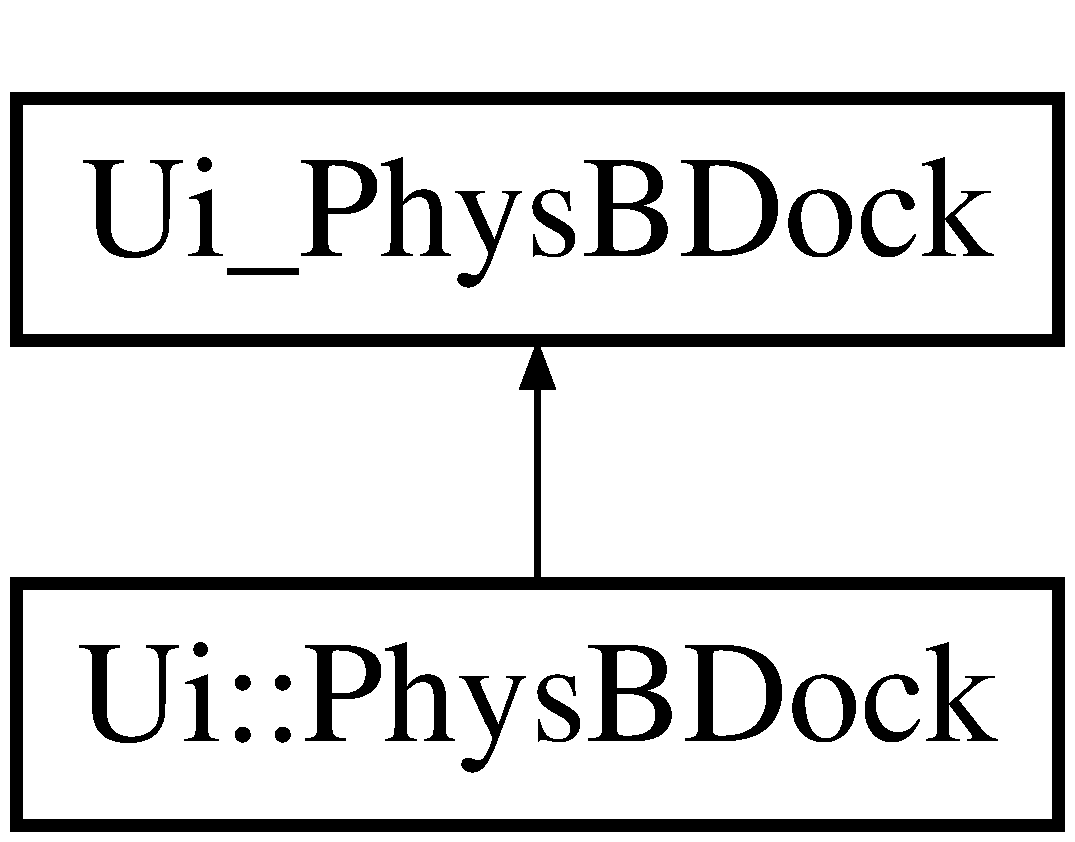
\includegraphics[height=2.000000cm]{class_ui___phys_b_dock}
\end{center}
\end{figure}
\subsection*{Public Member Functions}
\begin{DoxyCompactItemize}
\item 
void \hyperlink{class_ui___phys_b_dock_a335ee69ced7a7c0402c18b55f5e8b2d0}{setup\-Ui} (Q\-Dock\-Widget $\ast$Phys\-B\-Dock)
\item 
void \hyperlink{class_ui___phys_b_dock_abc5108323e77b2e0a5ea5d18ae1c8f93}{retranslate\-Ui} (Q\-Dock\-Widget $\ast$Phys\-B\-Dock)
\end{DoxyCompactItemize}
\subsection*{Public Attributes}
\begin{DoxyCompactItemize}
\item 
Q\-Widget $\ast$ \hyperlink{class_ui___phys_b_dock_afb820b26a533843d9c568c6c91df0021}{dock\-Widget\-Contents}
\item 
Q\-Push\-Button $\ast$ \hyperlink{class_ui___phys_b_dock_a011f24bbe2ada22ad04c4da81c72c3b1}{phys\-B\-Button}
\item 
Q\-Frame $\ast$ \hyperlink{class_ui___phys_b_dock_ac5cc5c7e3a4d3c418afac6754b5e2824}{line}
\item 
Q\-Frame $\ast$ \hyperlink{class_ui___phys_b_dock_a37156c5e0a99eee9ffc0bbf3aae14289}{line\-\_\-2}
\end{DoxyCompactItemize}


\subsection{Member Function Documentation}
\hypertarget{class_ui___phys_b_dock_abc5108323e77b2e0a5ea5d18ae1c8f93}{\index{Ui\-\_\-\-Phys\-B\-Dock@{Ui\-\_\-\-Phys\-B\-Dock}!retranslate\-Ui@{retranslate\-Ui}}
\index{retranslate\-Ui@{retranslate\-Ui}!Ui_PhysBDock@{Ui\-\_\-\-Phys\-B\-Dock}}
\subsubsection[{retranslate\-Ui}]{\setlength{\rightskip}{0pt plus 5cm}void Ui\-\_\-\-Phys\-B\-Dock\-::retranslate\-Ui (
\begin{DoxyParamCaption}
\item[{Q\-Dock\-Widget $\ast$}]{Phys\-B\-Dock}
\end{DoxyParamCaption}
)\hspace{0.3cm}{\ttfamily [inline]}}}\label{class_ui___phys_b_dock_abc5108323e77b2e0a5ea5d18ae1c8f93}
\hypertarget{class_ui___phys_b_dock_a335ee69ced7a7c0402c18b55f5e8b2d0}{\index{Ui\-\_\-\-Phys\-B\-Dock@{Ui\-\_\-\-Phys\-B\-Dock}!setup\-Ui@{setup\-Ui}}
\index{setup\-Ui@{setup\-Ui}!Ui_PhysBDock@{Ui\-\_\-\-Phys\-B\-Dock}}
\subsubsection[{setup\-Ui}]{\setlength{\rightskip}{0pt plus 5cm}void Ui\-\_\-\-Phys\-B\-Dock\-::setup\-Ui (
\begin{DoxyParamCaption}
\item[{Q\-Dock\-Widget $\ast$}]{Phys\-B\-Dock}
\end{DoxyParamCaption}
)\hspace{0.3cm}{\ttfamily [inline]}}}\label{class_ui___phys_b_dock_a335ee69ced7a7c0402c18b55f5e8b2d0}


\subsection{Member Data Documentation}
\hypertarget{class_ui___phys_b_dock_afb820b26a533843d9c568c6c91df0021}{\index{Ui\-\_\-\-Phys\-B\-Dock@{Ui\-\_\-\-Phys\-B\-Dock}!dock\-Widget\-Contents@{dock\-Widget\-Contents}}
\index{dock\-Widget\-Contents@{dock\-Widget\-Contents}!Ui_PhysBDock@{Ui\-\_\-\-Phys\-B\-Dock}}
\subsubsection[{dock\-Widget\-Contents}]{\setlength{\rightskip}{0pt plus 5cm}Q\-Widget$\ast$ Ui\-\_\-\-Phys\-B\-Dock\-::dock\-Widget\-Contents}}\label{class_ui___phys_b_dock_afb820b26a533843d9c568c6c91df0021}
\hypertarget{class_ui___phys_b_dock_ac5cc5c7e3a4d3c418afac6754b5e2824}{\index{Ui\-\_\-\-Phys\-B\-Dock@{Ui\-\_\-\-Phys\-B\-Dock}!line@{line}}
\index{line@{line}!Ui_PhysBDock@{Ui\-\_\-\-Phys\-B\-Dock}}
\subsubsection[{line}]{\setlength{\rightskip}{0pt plus 5cm}Q\-Frame$\ast$ Ui\-\_\-\-Phys\-B\-Dock\-::line}}\label{class_ui___phys_b_dock_ac5cc5c7e3a4d3c418afac6754b5e2824}
\hypertarget{class_ui___phys_b_dock_a37156c5e0a99eee9ffc0bbf3aae14289}{\index{Ui\-\_\-\-Phys\-B\-Dock@{Ui\-\_\-\-Phys\-B\-Dock}!line\-\_\-2@{line\-\_\-2}}
\index{line\-\_\-2@{line\-\_\-2}!Ui_PhysBDock@{Ui\-\_\-\-Phys\-B\-Dock}}
\subsubsection[{line\-\_\-2}]{\setlength{\rightskip}{0pt plus 5cm}Q\-Frame$\ast$ Ui\-\_\-\-Phys\-B\-Dock\-::line\-\_\-2}}\label{class_ui___phys_b_dock_a37156c5e0a99eee9ffc0bbf3aae14289}
\hypertarget{class_ui___phys_b_dock_a011f24bbe2ada22ad04c4da81c72c3b1}{\index{Ui\-\_\-\-Phys\-B\-Dock@{Ui\-\_\-\-Phys\-B\-Dock}!phys\-B\-Button@{phys\-B\-Button}}
\index{phys\-B\-Button@{phys\-B\-Button}!Ui_PhysBDock@{Ui\-\_\-\-Phys\-B\-Dock}}
\subsubsection[{phys\-B\-Button}]{\setlength{\rightskip}{0pt plus 5cm}Q\-Push\-Button$\ast$ Ui\-\_\-\-Phys\-B\-Dock\-::phys\-B\-Button}}\label{class_ui___phys_b_dock_a011f24bbe2ada22ad04c4da81c72c3b1}


The documentation for this class was generated from the following file\-:\begin{DoxyCompactItemize}
\item 
D\-:/\-Development/\-My\-Projects/\-Physically\-Based\-Modeling/include/\hyperlink{ui___physically_based_8h}{ui\-\_\-\-Physically\-Based.\-h}\end{DoxyCompactItemize}

\hypertarget{class_vector2_d}{\section{Vector2\-D Class Reference}
\label{class_vector2_d}\index{Vector2\-D@{Vector2\-D}}
}


{\ttfamily \#include $<$Utility.\-h$>$}

\subsection*{Public Member Functions}
\begin{DoxyCompactItemize}
\item 
\hyperlink{class_vector2_d_a98e9997ebb7a629f4db52397d4e0d653}{Vector2\-D} ()
\item 
\hyperlink{class_vector2_d_a525e125aac4c844f04c52ddb0e75d594}{Vector2\-D} (double x, double y)
\item 
std\-::string \hyperlink{class_vector2_d_a3a5733c80b717c907b43b755e94625ef}{to\-String} () const 
\end{DoxyCompactItemize}
\subsection*{Public Attributes}
\begin{DoxyCompactItemize}
\item 
double \hyperlink{class_vector2_d_a3bdf405eacce2d6efe0ea3d9b80bede5}{elements} \mbox{[}size\mbox{]}
\end{DoxyCompactItemize}


\subsection{Constructor \& Destructor Documentation}
\hypertarget{class_vector2_d_a98e9997ebb7a629f4db52397d4e0d653}{\index{Vector2\-D@{Vector2\-D}!Vector2\-D@{Vector2\-D}}
\index{Vector2\-D@{Vector2\-D}!Vector2D@{Vector2\-D}}
\subsubsection[{Vector2\-D}]{\setlength{\rightskip}{0pt plus 5cm}Vector2\-D\-::\-Vector2\-D (
\begin{DoxyParamCaption}
{}
\end{DoxyParamCaption}
)\hspace{0.3cm}{\ttfamily [inline]}}}\label{class_vector2_d_a98e9997ebb7a629f4db52397d4e0d653}
\hypertarget{class_vector2_d_a525e125aac4c844f04c52ddb0e75d594}{\index{Vector2\-D@{Vector2\-D}!Vector2\-D@{Vector2\-D}}
\index{Vector2\-D@{Vector2\-D}!Vector2D@{Vector2\-D}}
\subsubsection[{Vector2\-D}]{\setlength{\rightskip}{0pt plus 5cm}Vector2\-D\-::\-Vector2\-D (
\begin{DoxyParamCaption}
\item[{double}]{x, }
\item[{double}]{y}
\end{DoxyParamCaption}
)\hspace{0.3cm}{\ttfamily [inline]}}}\label{class_vector2_d_a525e125aac4c844f04c52ddb0e75d594}


\subsection{Member Function Documentation}
\hypertarget{class_vector2_d_a3a5733c80b717c907b43b755e94625ef}{\index{Vector2\-D@{Vector2\-D}!to\-String@{to\-String}}
\index{to\-String@{to\-String}!Vector2D@{Vector2\-D}}
\subsubsection[{to\-String}]{\setlength{\rightskip}{0pt plus 5cm}std\-::string Vector2\-D\-::to\-String (
\begin{DoxyParamCaption}
{}
\end{DoxyParamCaption}
) const\hspace{0.3cm}{\ttfamily [inline]}}}\label{class_vector2_d_a3a5733c80b717c907b43b755e94625ef}


\subsection{Member Data Documentation}
\hypertarget{class_vector2_d_a3bdf405eacce2d6efe0ea3d9b80bede5}{\index{Vector2\-D@{Vector2\-D}!elements@{elements}}
\index{elements@{elements}!Vector2D@{Vector2\-D}}
\subsubsection[{elements}]{\setlength{\rightskip}{0pt plus 5cm}double Vector2\-D\-::elements\mbox{[}size\mbox{]}}}\label{class_vector2_d_a3bdf405eacce2d6efe0ea3d9b80bede5}


The documentation for this class was generated from the following file\-:\begin{DoxyCompactItemize}
\item 
D\-:/\-Development/\-My\-Projects/\-Physically\-Based\-Modeling/include/\hyperlink{_utility_8h}{Utility.\-h}\end{DoxyCompactItemize}

\hypertarget{class_vector3_d}{\section{Vector3\-D Class Reference}
\label{class_vector3_d}\index{Vector3\-D@{Vector3\-D}}
}


{\ttfamily \#include $<$Utility.\-h$>$}

\subsection*{Public Member Functions}
\begin{DoxyCompactItemize}
\item 
\hyperlink{class_vector3_d_a0b11a8d75da427b27443d8a94d0d296c}{Vector3\-D} ()
\item 
\hyperlink{class_vector3_d_abd851542da40b1168edcad11fa83b7c2}{Vector3\-D} (double x, double y, double z)
\item 
double \hyperlink{class_vector3_d_a9e900adfd823b6293f1bf01d84b9fff6}{calc\-Magnitude} () const 
\item 
\hyperlink{class_vector3_d}{Vector3\-D} \hyperlink{class_vector3_d_a5b3059961eb8b4db3dc6b79f283dcac1}{normalize} () const 
\item 
\hyperlink{class_vector3_d}{Vector3\-D} \& \hyperlink{class_vector3_d_a65c133291142447f6bdbdc4425303078}{operator=} (const \hyperlink{class_vector3_d}{Vector3\-D} \&rhs)
\item 
\hyperlink{class_vector3_d}{Vector3\-D} \& \hyperlink{class_vector3_d_a3448ab3b394051519147d76647e7f006}{operator+=} (const \hyperlink{class_vector3_d}{Vector3\-D} \&rhs)
\item 
\hyperlink{class_vector3_d}{Vector3\-D} \& \hyperlink{class_vector3_d_a571ef878a82e754c9280c9f4eb2d990b}{operator-\/=} (const \hyperlink{class_vector3_d}{Vector3\-D} \&rhs)
\item 
\hyperlink{class_vector3_d}{Vector3\-D} \hyperlink{class_vector3_d_a03f189f8d45eda497772364d19d30c7d}{operator-\/} () const 
\item 
double \hyperlink{class_vector3_d_a9eea2c879cc0721b71925088fecbab9c}{dot\-Product} (const \hyperlink{class_vector3_d}{Vector3\-D} \&v) const 
\item 
\hyperlink{class_vector3_d}{Vector3\-D} \hyperlink{class_vector3_d_a39ad41be410fec3615f471bde6e17321}{cross\-Product} (const \hyperlink{class_vector3_d}{Vector3\-D} \&v)
\item 
std\-::string \hyperlink{class_vector3_d_a37dfc4a95d1af4ce314852b54a2f6227}{to\-String} () const 
\end{DoxyCompactItemize}
\subsection*{Public Attributes}
\begin{DoxyCompactItemize}
\item 
double \hyperlink{class_vector3_d_a3c92dcba304b8b23c9961eb5ccfbed63}{elements} \mbox{[}size\mbox{]}
\end{DoxyCompactItemize}
\subsection*{Friends}
\begin{DoxyCompactItemize}
\item 
\hyperlink{class_vector3_d}{Vector3\-D} \hyperlink{class_vector3_d_ac6411f933860f0e12b87da2ec1698197}{operator+} (const \hyperlink{class_vector3_d}{Vector3\-D} \&v1, const \hyperlink{class_vector3_d}{Vector3\-D} \&v2)
\item 
\hyperlink{class_vector3_d}{Vector3\-D} \hyperlink{class_vector3_d_ae2b0c437a1ccad22fc33fd9750079e5e}{operator-\/} (const \hyperlink{class_vector3_d}{Vector3\-D} \&v1, const \hyperlink{class_vector3_d}{Vector3\-D} \&v2)
\item 
\hyperlink{class_vector3_d}{Vector3\-D} \hyperlink{class_vector3_d_a37a1cbe0594313bd52fe13f50011add1}{operator$\ast$} (const \hyperlink{class_vector3_d}{Vector3\-D} \&v1, const double s)
\item 
\hyperlink{class_vector3_d}{Vector3\-D} \hyperlink{class_vector3_d_ab833cc21e16fad258cc5445e7798aea4}{operator/} (const \hyperlink{class_vector3_d}{Vector3\-D} \&v1, const double s)
\item 
\hyperlink{class_vector3_d}{Vector3\-D} \hyperlink{class_vector3_d_a7ab094401d4017867594d9e321bde89c}{operator$\ast$} (const \hyperlink{class_matrix3_d}{Matrix3\-D} \&s, const \hyperlink{class_vector3_d}{Vector3\-D} \&v)
\item 
\hyperlink{class_vector3_d}{Vector3\-D} \hyperlink{class_vector3_d_afd02bcb799e94637ae32829e62d519b8}{m\-\_\-mult\-\_\-dir\-Vec} (const \hyperlink{class_matrix3_d}{Matrix3\-D} \&s, const \hyperlink{class_vector3_d}{Vector3\-D} \&v)
\end{DoxyCompactItemize}


\subsection{Constructor \& Destructor Documentation}
\hypertarget{class_vector3_d_a0b11a8d75da427b27443d8a94d0d296c}{\index{Vector3\-D@{Vector3\-D}!Vector3\-D@{Vector3\-D}}
\index{Vector3\-D@{Vector3\-D}!Vector3D@{Vector3\-D}}
\subsubsection[{Vector3\-D}]{\setlength{\rightskip}{0pt plus 5cm}Vector3\-D\-::\-Vector3\-D (
\begin{DoxyParamCaption}
{}
\end{DoxyParamCaption}
)}}\label{class_vector3_d_a0b11a8d75da427b27443d8a94d0d296c}
\hypertarget{class_vector3_d_abd851542da40b1168edcad11fa83b7c2}{\index{Vector3\-D@{Vector3\-D}!Vector3\-D@{Vector3\-D}}
\index{Vector3\-D@{Vector3\-D}!Vector3D@{Vector3\-D}}
\subsubsection[{Vector3\-D}]{\setlength{\rightskip}{0pt plus 5cm}Vector3\-D\-::\-Vector3\-D (
\begin{DoxyParamCaption}
\item[{double}]{x, }
\item[{double}]{y, }
\item[{double}]{z}
\end{DoxyParamCaption}
)}}\label{class_vector3_d_abd851542da40b1168edcad11fa83b7c2}


\subsection{Member Function Documentation}
\hypertarget{class_vector3_d_a9e900adfd823b6293f1bf01d84b9fff6}{\index{Vector3\-D@{Vector3\-D}!calc\-Magnitude@{calc\-Magnitude}}
\index{calc\-Magnitude@{calc\-Magnitude}!Vector3D@{Vector3\-D}}
\subsubsection[{calc\-Magnitude}]{\setlength{\rightskip}{0pt plus 5cm}double Vector3\-D\-::calc\-Magnitude (
\begin{DoxyParamCaption}
{}
\end{DoxyParamCaption}
) const}}\label{class_vector3_d_a9e900adfd823b6293f1bf01d84b9fff6}
\hypertarget{class_vector3_d_a39ad41be410fec3615f471bde6e17321}{\index{Vector3\-D@{Vector3\-D}!cross\-Product@{cross\-Product}}
\index{cross\-Product@{cross\-Product}!Vector3D@{Vector3\-D}}
\subsubsection[{cross\-Product}]{\setlength{\rightskip}{0pt plus 5cm}{\bf Vector3\-D} Vector3\-D\-::cross\-Product (
\begin{DoxyParamCaption}
\item[{const {\bf Vector3\-D} \&}]{v}
\end{DoxyParamCaption}
)}}\label{class_vector3_d_a39ad41be410fec3615f471bde6e17321}
\hypertarget{class_vector3_d_a9eea2c879cc0721b71925088fecbab9c}{\index{Vector3\-D@{Vector3\-D}!dot\-Product@{dot\-Product}}
\index{dot\-Product@{dot\-Product}!Vector3D@{Vector3\-D}}
\subsubsection[{dot\-Product}]{\setlength{\rightskip}{0pt plus 5cm}double Vector3\-D\-::dot\-Product (
\begin{DoxyParamCaption}
\item[{const {\bf Vector3\-D} \&}]{v}
\end{DoxyParamCaption}
) const}}\label{class_vector3_d_a9eea2c879cc0721b71925088fecbab9c}
\hypertarget{class_vector3_d_a5b3059961eb8b4db3dc6b79f283dcac1}{\index{Vector3\-D@{Vector3\-D}!normalize@{normalize}}
\index{normalize@{normalize}!Vector3D@{Vector3\-D}}
\subsubsection[{normalize}]{\setlength{\rightskip}{0pt plus 5cm}{\bf Vector3\-D} Vector3\-D\-::normalize (
\begin{DoxyParamCaption}
{}
\end{DoxyParamCaption}
) const}}\label{class_vector3_d_a5b3059961eb8b4db3dc6b79f283dcac1}
\hypertarget{class_vector3_d_a3448ab3b394051519147d76647e7f006}{\index{Vector3\-D@{Vector3\-D}!operator+=@{operator+=}}
\index{operator+=@{operator+=}!Vector3D@{Vector3\-D}}
\subsubsection[{operator+=}]{\setlength{\rightskip}{0pt plus 5cm}{\bf Vector3\-D}\& Vector3\-D\-::operator+= (
\begin{DoxyParamCaption}
\item[{const {\bf Vector3\-D} \&}]{rhs}
\end{DoxyParamCaption}
)}}\label{class_vector3_d_a3448ab3b394051519147d76647e7f006}
\hypertarget{class_vector3_d_a03f189f8d45eda497772364d19d30c7d}{\index{Vector3\-D@{Vector3\-D}!operator-\/@{operator-\/}}
\index{operator-\/@{operator-\/}!Vector3D@{Vector3\-D}}
\subsubsection[{operator-\/}]{\setlength{\rightskip}{0pt plus 5cm}{\bf Vector3\-D} Vector3\-D\-::operator-\/ (
\begin{DoxyParamCaption}
{}
\end{DoxyParamCaption}
) const}}\label{class_vector3_d_a03f189f8d45eda497772364d19d30c7d}
\hypertarget{class_vector3_d_a571ef878a82e754c9280c9f4eb2d990b}{\index{Vector3\-D@{Vector3\-D}!operator-\/=@{operator-\/=}}
\index{operator-\/=@{operator-\/=}!Vector3D@{Vector3\-D}}
\subsubsection[{operator-\/=}]{\setlength{\rightskip}{0pt plus 5cm}{\bf Vector3\-D}\& Vector3\-D\-::operator-\/= (
\begin{DoxyParamCaption}
\item[{const {\bf Vector3\-D} \&}]{rhs}
\end{DoxyParamCaption}
)}}\label{class_vector3_d_a571ef878a82e754c9280c9f4eb2d990b}
\hypertarget{class_vector3_d_a65c133291142447f6bdbdc4425303078}{\index{Vector3\-D@{Vector3\-D}!operator=@{operator=}}
\index{operator=@{operator=}!Vector3D@{Vector3\-D}}
\subsubsection[{operator=}]{\setlength{\rightskip}{0pt plus 5cm}{\bf Vector3\-D}\& Vector3\-D\-::operator= (
\begin{DoxyParamCaption}
\item[{const {\bf Vector3\-D} \&}]{rhs}
\end{DoxyParamCaption}
)}}\label{class_vector3_d_a65c133291142447f6bdbdc4425303078}
\hypertarget{class_vector3_d_a37dfc4a95d1af4ce314852b54a2f6227}{\index{Vector3\-D@{Vector3\-D}!to\-String@{to\-String}}
\index{to\-String@{to\-String}!Vector3D@{Vector3\-D}}
\subsubsection[{to\-String}]{\setlength{\rightskip}{0pt plus 5cm}std\-::string Vector3\-D\-::to\-String (
\begin{DoxyParamCaption}
{}
\end{DoxyParamCaption}
) const\hspace{0.3cm}{\ttfamily [inline]}}}\label{class_vector3_d_a37dfc4a95d1af4ce314852b54a2f6227}


\subsection{Friends And Related Function Documentation}
\hypertarget{class_vector3_d_afd02bcb799e94637ae32829e62d519b8}{\index{Vector3\-D@{Vector3\-D}!m\-\_\-mult\-\_\-dir\-Vec@{m\-\_\-mult\-\_\-dir\-Vec}}
\index{m\-\_\-mult\-\_\-dir\-Vec@{m\-\_\-mult\-\_\-dir\-Vec}!Vector3D@{Vector3\-D}}
\subsubsection[{m\-\_\-mult\-\_\-dir\-Vec}]{\setlength{\rightskip}{0pt plus 5cm}{\bf Vector3\-D} m\-\_\-mult\-\_\-dir\-Vec (
\begin{DoxyParamCaption}
\item[{const {\bf Matrix3\-D} \&}]{s, }
\item[{const {\bf Vector3\-D} \&}]{v}
\end{DoxyParamCaption}
)\hspace{0.3cm}{\ttfamily [friend]}}}\label{class_vector3_d_afd02bcb799e94637ae32829e62d519b8}
\hypertarget{class_vector3_d_a37a1cbe0594313bd52fe13f50011add1}{\index{Vector3\-D@{Vector3\-D}!operator$\ast$@{operator$\ast$}}
\index{operator$\ast$@{operator$\ast$}!Vector3D@{Vector3\-D}}
\subsubsection[{operator$\ast$}]{\setlength{\rightskip}{0pt plus 5cm}{\bf Vector3\-D} operator$\ast$ (
\begin{DoxyParamCaption}
\item[{const {\bf Vector3\-D} \&}]{v1, }
\item[{const double}]{s}
\end{DoxyParamCaption}
)\hspace{0.3cm}{\ttfamily [friend]}}}\label{class_vector3_d_a37a1cbe0594313bd52fe13f50011add1}
\hypertarget{class_vector3_d_a7ab094401d4017867594d9e321bde89c}{\index{Vector3\-D@{Vector3\-D}!operator$\ast$@{operator$\ast$}}
\index{operator$\ast$@{operator$\ast$}!Vector3D@{Vector3\-D}}
\subsubsection[{operator$\ast$}]{\setlength{\rightskip}{0pt plus 5cm}{\bf Vector3\-D} operator$\ast$ (
\begin{DoxyParamCaption}
\item[{const {\bf Matrix3\-D} \&}]{s, }
\item[{const {\bf Vector3\-D} \&}]{v}
\end{DoxyParamCaption}
)\hspace{0.3cm}{\ttfamily [friend]}}}\label{class_vector3_d_a7ab094401d4017867594d9e321bde89c}
\hypertarget{class_vector3_d_ac6411f933860f0e12b87da2ec1698197}{\index{Vector3\-D@{Vector3\-D}!operator+@{operator+}}
\index{operator+@{operator+}!Vector3D@{Vector3\-D}}
\subsubsection[{operator+}]{\setlength{\rightskip}{0pt plus 5cm}{\bf Vector3\-D} operator+ (
\begin{DoxyParamCaption}
\item[{const {\bf Vector3\-D} \&}]{v1, }
\item[{const {\bf Vector3\-D} \&}]{v2}
\end{DoxyParamCaption}
)\hspace{0.3cm}{\ttfamily [friend]}}}\label{class_vector3_d_ac6411f933860f0e12b87da2ec1698197}
\hypertarget{class_vector3_d_ae2b0c437a1ccad22fc33fd9750079e5e}{\index{Vector3\-D@{Vector3\-D}!operator-\/@{operator-\/}}
\index{operator-\/@{operator-\/}!Vector3D@{Vector3\-D}}
\subsubsection[{operator-\/}]{\setlength{\rightskip}{0pt plus 5cm}{\bf Vector3\-D} operator-\/ (
\begin{DoxyParamCaption}
\item[{const {\bf Vector3\-D} \&}]{v1, }
\item[{const {\bf Vector3\-D} \&}]{v2}
\end{DoxyParamCaption}
)\hspace{0.3cm}{\ttfamily [friend]}}}\label{class_vector3_d_ae2b0c437a1ccad22fc33fd9750079e5e}
\hypertarget{class_vector3_d_ab833cc21e16fad258cc5445e7798aea4}{\index{Vector3\-D@{Vector3\-D}!operator/@{operator/}}
\index{operator/@{operator/}!Vector3D@{Vector3\-D}}
\subsubsection[{operator/}]{\setlength{\rightskip}{0pt plus 5cm}{\bf Vector3\-D} operator/ (
\begin{DoxyParamCaption}
\item[{const {\bf Vector3\-D} \&}]{v1, }
\item[{const double}]{s}
\end{DoxyParamCaption}
)\hspace{0.3cm}{\ttfamily [friend]}}}\label{class_vector3_d_ab833cc21e16fad258cc5445e7798aea4}


\subsection{Member Data Documentation}
\hypertarget{class_vector3_d_a3c92dcba304b8b23c9961eb5ccfbed63}{\index{Vector3\-D@{Vector3\-D}!elements@{elements}}
\index{elements@{elements}!Vector3D@{Vector3\-D}}
\subsubsection[{elements}]{\setlength{\rightskip}{0pt plus 5cm}double Vector3\-D\-::elements\mbox{[}size\mbox{]}}}\label{class_vector3_d_a3c92dcba304b8b23c9961eb5ccfbed63}


The documentation for this class was generated from the following file\-:\begin{DoxyCompactItemize}
\item 
D\-:/\-Development/\-My\-Projects/\-Physically\-Based\-Modeling/include/\hyperlink{_utility_8h}{Utility.\-h}\end{DoxyCompactItemize}

\chapter{File Documentation}
\hypertarget{_application_8h}{\section{D\-:/\-Development/\-My\-Projects/\-Physically\-Based\-Modeling/include/\-Application.h File Reference}
\label{_application_8h}\index{D\-:/\-Development/\-My\-Projects/\-Physically\-Based\-Modeling/include/\-Application.\-h@{D\-:/\-Development/\-My\-Projects/\-Physically\-Based\-Modeling/include/\-Application.\-h}}
}
{\ttfamily \#include $<$iostream$>$}\\*
{\ttfamily \#include $<$fstream$>$}\\*
{\ttfamily \#include $<$sstream$>$}\\*
{\ttfamily \#include $<$Q\-Main\-Window$>$}\\*
{\ttfamily \#include $<$Qt\-Gui$>$}\\*
{\ttfamily \#include $<$S\-F\-M\-L/\-System.\-hpp$>$}\\*
{\ttfamily \#include $<$S\-F\-M\-L/\-Graphics.\-hpp$>$}\\*
{\ttfamily \#include $<$S\-F\-M\-L/\-Window.\-hpp$>$}\\*
{\ttfamily \#include $<$S\-F\-M\-L/\-Open\-G\-L.\-hpp$>$}\\*
{\ttfamily \#include $<$Physically\-Based.\-h$>$}\\*
{\ttfamily \#include $<$ui\-\_\-\-Physically\-Based.\-h$>$}\\*
\subsection*{Classes}
\begin{DoxyCompactItemize}
\item 
class \hyperlink{class_application}{Application}
\end{DoxyCompactItemize}

\hypertarget{_box_8h}{\section{D\-:/\-Development/\-My\-Projects/\-Physically\-Based\-Modeling/include/\-Box.h File Reference}
\label{_box_8h}\index{D\-:/\-Development/\-My\-Projects/\-Physically\-Based\-Modeling/include/\-Box.\-h@{D\-:/\-Development/\-My\-Projects/\-Physically\-Based\-Modeling/include/\-Box.\-h}}
}
{\ttfamily \#include $<$Shape.\-h$>$}\\*
{\ttfamily \#include $<$Utility.\-h$>$}\\*
\subsection*{Classes}
\begin{DoxyCompactItemize}
\item 
class \hyperlink{class_box}{Box}
\end{DoxyCompactItemize}

\hypertarget{_collidable_object_8h}{\section{D\-:/\-Development/\-My\-Projects/\-Physically\-Based\-Modeling/include/\-Collidable\-Object.h File Reference}
\label{_collidable_object_8h}\index{D\-:/\-Development/\-My\-Projects/\-Physically\-Based\-Modeling/include/\-Collidable\-Object.\-h@{D\-:/\-Development/\-My\-Projects/\-Physically\-Based\-Modeling/include/\-Collidable\-Object.\-h}}
}
{\ttfamily \#include $<$Object.\-h$>$}\\*
\subsection*{Classes}
\begin{DoxyCompactItemize}
\item 
class \hyperlink{class_collision_force}{Collision\-Force}
\item 
class \hyperlink{class_deferred_force}{Deferred\-Force}
\item 
class \hyperlink{class_collidable_object}{Collidable\-Object}
\end{DoxyCompactItemize}

\hypertarget{_collider_object_8h}{\section{D\-:/\-Development/\-My\-Projects/\-Physically\-Based\-Modeling/include/\-Collider\-Object.h File Reference}
\label{_collider_object_8h}\index{D\-:/\-Development/\-My\-Projects/\-Physically\-Based\-Modeling/include/\-Collider\-Object.\-h@{D\-:/\-Development/\-My\-Projects/\-Physically\-Based\-Modeling/include/\-Collider\-Object.\-h}}
}
{\ttfamily \#include $<$Collidable\-Object.\-h$>$}\\*
\subsection*{Classes}
\begin{DoxyCompactItemize}
\item 
class \hyperlink{class_simple_deferred_force}{Simple\-Deferred\-Force}
\item 
class \hyperlink{class_collider_object}{Collider\-Object}
\end{DoxyCompactItemize}

\hypertarget{_collision_handler_8h}{\section{D\-:/\-Development/\-My\-Projects/\-Physically\-Based\-Modeling/include/\-Collision\-Handler.h File Reference}
\label{_collision_handler_8h}\index{D\-:/\-Development/\-My\-Projects/\-Physically\-Based\-Modeling/include/\-Collision\-Handler.\-h@{D\-:/\-Development/\-My\-Projects/\-Physically\-Based\-Modeling/include/\-Collision\-Handler.\-h}}
}
{\ttfamily \#include $<$cmath$>$}\\*
{\ttfamily \#include $<$Quad\-Plane.\-h$>$}\\*
{\ttfamily \#include $<$Sphere.\-h$>$}\\*
\subsection*{Namespaces}
\begin{DoxyCompactItemize}
\item 
\hyperlink{namespace_collision_handler}{Collision\-Handler}
\end{DoxyCompactItemize}
\subsection*{Functions}
\begin{DoxyCompactItemize}
\item 
bool \hyperlink{namespace_collision_handler_a745096d27ac0c37c74f82334184b73db}{Collision\-Handler\-::collision} (const \hyperlink{class_quad_plane}{Quad\-Plane} \&qp, const \hyperlink{class_transform}{Transform} \&qp\-\_\-new\-Tr, const \hyperlink{class_sphere}{Sphere} \&s, const \hyperlink{class_transform}{Transform} \&s\-\_\-new\-Tr, float $\ast$timestep\-Frac, \hyperlink{class_vector3_d}{Vector3\-D} $\ast$collision\-Normal)
\item 
bool \hyperlink{namespace_collision_handler_abdf4d543db8d5f6fc012ff91f31f2140}{Collision\-Handler\-::collision} (const \hyperlink{class_sphere}{Sphere} \&s, const \hyperlink{class_vector3_d}{Vector3\-D} \&s\-\_\-p0, const \hyperlink{class_vector3_d}{Vector3\-D} \&s\-\_\-p1, const \hyperlink{class_quad_plane}{Quad\-Plane} \&qp, const \hyperlink{class_vector3_d}{Vector3\-D} \&qp\-\_\-p0, const \hyperlink{class_vector3_d}{Vector3\-D} \&qp\-\_\-p1, float $\ast$timestep\-Frac, \hyperlink{class_vector3_d}{Vector3\-D} $\ast$collision\-Normal)
\item 
bool \hyperlink{namespace_collision_handler_a1bfa74edc99009c5e18c44df30ead02f}{Collision\-Handler\-::collision} (const \hyperlink{class_sphere}{Sphere} \&s0, const \hyperlink{class_vector3_d}{Vector3\-D} \&s0\-\_\-p0, const \hyperlink{class_vector3_d}{Vector3\-D} \&s0\-\_\-p1, const \hyperlink{class_sphere}{Sphere} \&s1, const \hyperlink{class_vector3_d}{Vector3\-D} \&s1\-\_\-p0, const \hyperlink{class_vector3_d}{Vector3\-D} \&s1\-\_\-p1, float $\ast$timestep\-Frac, \hyperlink{class_vector3_d}{Vector3\-D} $\ast$collision\-Normal)
\item 
bool \hyperlink{namespace_collision_handler_ac02fa6575701dd41985e32674370dbf2}{Collision\-Handler\-::collision} (const \hyperlink{class_quad_plane}{Quad\-Plane} \&s0, const \hyperlink{class_vector3_d}{Vector3\-D} \&qp0\-\_\-p0, const \hyperlink{class_vector3_d}{Vector3\-D} \&qp0\-\_\-p1, const \hyperlink{class_quad_plane}{Quad\-Plane} \&s1, const \hyperlink{class_vector3_d}{Vector3\-D} \&qp1\-\_\-p0, const \hyperlink{class_vector3_d}{Vector3\-D} \&qp1\-\_\-p1, float $\ast$timestep\-Frac, \hyperlink{class_vector3_d}{Vector3\-D} $\ast$collision\-Normal)
\end{DoxyCompactItemize}

\hypertarget{_environment_8h}{\section{D\-:/\-Development/\-My\-Projects/\-Physically\-Based\-Modeling/include/\-Environment.h File Reference}
\label{_environment_8h}\index{D\-:/\-Development/\-My\-Projects/\-Physically\-Based\-Modeling/include/\-Environment.\-h@{D\-:/\-Development/\-My\-Projects/\-Physically\-Based\-Modeling/include/\-Environment.\-h}}
}
{\ttfamily \#include $<$Force\-Environment.\-h$>$}\\*
\subsection*{Classes}
\begin{DoxyCompactItemize}
\item 
class \hyperlink{class_environment}{Environment}
\end{DoxyCompactItemize}

\hypertarget{_events_8h}{\section{D\-:/\-Development/\-My\-Projects/\-Physically\-Based\-Modeling/include/\-Events.h File Reference}
\label{_events_8h}\index{D\-:/\-Development/\-My\-Projects/\-Physically\-Based\-Modeling/include/\-Events.\-h@{D\-:/\-Development/\-My\-Projects/\-Physically\-Based\-Modeling/include/\-Events.\-h}}
}
{\ttfamily \#include $<$Q\-Event$>$}\\*
\subsection*{Classes}
\begin{DoxyCompactItemize}
\item 
class \hyperlink{class_phys_b_event}{Phys\-B\-Event}
\end{DoxyCompactItemize}

\hypertarget{_force_8h}{\section{D\-:/\-Development/\-My\-Projects/\-Physically\-Based\-Modeling/include/\-Force.h File Reference}
\label{_force_8h}\index{D\-:/\-Development/\-My\-Projects/\-Physically\-Based\-Modeling/include/\-Force.\-h@{D\-:/\-Development/\-My\-Projects/\-Physically\-Based\-Modeling/include/\-Force.\-h}}
}
\subsection*{Classes}
\begin{DoxyCompactItemize}
\item 
class \hyperlink{class_force}{Force}
\item 
class \hyperlink{class_independent_force}{Independent\-Force}
\end{DoxyCompactItemize}
\subsection*{Functions}
\begin{DoxyCompactItemize}
\item 
\hyperlink{class_independent_force}{Independent\-Force} \hyperlink{_force_8h_a2afa18d4bcd38d8a499ad886099feaff}{operator+} (\hyperlink{class_independent_force}{Independent\-Force} lhs, const \hyperlink{class_independent_force}{Independent\-Force} \&rhs)
\end{DoxyCompactItemize}


\subsection{Function Documentation}
\hypertarget{_force_8h_a2afa18d4bcd38d8a499ad886099feaff}{\index{Force.\-h@{Force.\-h}!operator+@{operator+}}
\index{operator+@{operator+}!Force.h@{Force.\-h}}
\subsubsection[{operator+}]{\setlength{\rightskip}{0pt plus 5cm}{\bf Independent\-Force} operator+ (
\begin{DoxyParamCaption}
\item[{{\bf Independent\-Force}}]{lhs, }
\item[{const {\bf Independent\-Force} \&}]{rhs}
\end{DoxyParamCaption}
)\hspace{0.3cm}{\ttfamily [inline]}}}\label{_force_8h_a2afa18d4bcd38d8a499ad886099feaff}

\hypertarget{_force_environment_8h}{\section{D\-:/\-Development/\-My\-Projects/\-Physically\-Based\-Modeling/include/\-Force\-Environment.h File Reference}
\label{_force_environment_8h}\index{D\-:/\-Development/\-My\-Projects/\-Physically\-Based\-Modeling/include/\-Force\-Environment.\-h@{D\-:/\-Development/\-My\-Projects/\-Physically\-Based\-Modeling/include/\-Force\-Environment.\-h}}
}
{\ttfamily \#include $<$vector$>$}\\*
{\ttfamily \#include $<$Force.\-h$>$}\\*
\subsection*{Classes}
\begin{DoxyCompactItemize}
\item 
class \hyperlink{class_force_environment}{Force\-Environment}
\end{DoxyCompactItemize}

\hypertarget{_q_s_f_m_l_canvas_8h}{\section{D\-:/\-Development/\-My\-Projects/\-Physically\-Based\-Modeling/include/\-G\-U\-I/\-Q\-S\-F\-M\-L\-Canvas.h File Reference}
\label{_q_s_f_m_l_canvas_8h}\index{D\-:/\-Development/\-My\-Projects/\-Physically\-Based\-Modeling/include/\-G\-U\-I/\-Q\-S\-F\-M\-L\-Canvas.\-h@{D\-:/\-Development/\-My\-Projects/\-Physically\-Based\-Modeling/include/\-G\-U\-I/\-Q\-S\-F\-M\-L\-Canvas.\-h}}
}
{\ttfamily \#include $<$S\-F\-M\-L/\-Open\-G\-L.\-hpp$>$}\\*
{\ttfamily \#include $<$G\-U\-I/render\-Window\-Wrapper.\-h$>$}\\*
{\ttfamily \#include $<$Q\-Widget$>$}\\*
{\ttfamily \#include $<$Q\-Timer$>$}\\*
\subsection*{Classes}
\begin{DoxyCompactItemize}
\item 
class \hyperlink{class_q_s_f_m_l_canvas}{Q\-S\-F\-M\-L\-Canvas}
\end{DoxyCompactItemize}

\hypertarget{render_window_wrapper_8h}{\section{D\-:/\-Development/\-My\-Projects/\-Physically\-Based\-Modeling/include/\-G\-U\-I/render\-Window\-Wrapper.h File Reference}
\label{render_window_wrapper_8h}\index{D\-:/\-Development/\-My\-Projects/\-Physically\-Based\-Modeling/include/\-G\-U\-I/render\-Window\-Wrapper.\-h@{D\-:/\-Development/\-My\-Projects/\-Physically\-Based\-Modeling/include/\-G\-U\-I/render\-Window\-Wrapper.\-h}}
}
{\ttfamily \#include $<$S\-F\-M\-L/\-Graphics.\-hpp$>$}\\*
\subsection*{Classes}
\begin{DoxyCompactItemize}
\item 
class \hyperlink{class_r_w_wrapper}{R\-W\-Wrapper}
\end{DoxyCompactItemize}

\hypertarget{_object_8h}{\section{D\-:/\-Development/\-My\-Projects/\-Physically\-Based\-Modeling/include/\-Object.h File Reference}
\label{_object_8h}\index{D\-:/\-Development/\-My\-Projects/\-Physically\-Based\-Modeling/include/\-Object.\-h@{D\-:/\-Development/\-My\-Projects/\-Physically\-Based\-Modeling/include/\-Object.\-h}}
}
{\ttfamily \#include $<$Utility.\-h$>$}\\*
{\ttfamily \#include $<$Transform.\-h$>$}\\*
{\ttfamily \#include $<$Renderable.\-h$>$}\\*
\subsection*{Classes}
\begin{DoxyCompactItemize}
\item 
class \hyperlink{class_object}{Object}
\end{DoxyCompactItemize}

\hypertarget{_physical_8h}{\section{D\-:/\-Development/\-My\-Projects/\-Physically\-Based\-Modeling/include/\-Physical.h File Reference}
\label{_physical_8h}\index{D\-:/\-Development/\-My\-Projects/\-Physically\-Based\-Modeling/include/\-Physical.\-h@{D\-:/\-Development/\-My\-Projects/\-Physically\-Based\-Modeling/include/\-Physical.\-h}}
}
\subsection*{Classes}
\begin{DoxyCompactItemize}
\item 
class \hyperlink{class_physical}{Physical}
\end{DoxyCompactItemize}

\hypertarget{_physically_based_8h}{\section{D\-:/\-Development/\-My\-Projects/\-Physically\-Based\-Modeling/include/\-Physically\-Based.h File Reference}
\label{_physically_based_8h}\index{D\-:/\-Development/\-My\-Projects/\-Physically\-Based\-Modeling/include/\-Physically\-Based.\-h@{D\-:/\-Development/\-My\-Projects/\-Physically\-Based\-Modeling/include/\-Physically\-Based.\-h}}
}
{\ttfamily \#include $<$Q\-Thread$>$}\\*
{\ttfamily \#include $<$vector$>$}\\*
{\ttfamily \#include $<$S\-F\-M\-L/\-Graphics.\-hpp$>$}\\*
{\ttfamily \#include $<$Utility.\-h$>$}\\*
{\ttfamily \#include $<$Environment.\-h$>$}\\*
\subsection*{Classes}
\begin{DoxyCompactItemize}
\item 
class \hyperlink{class_p_b_time}{P\-B\-Time}
\end{DoxyCompactItemize}
\subsection*{Functions}
\begin{DoxyCompactItemize}
\item 
class \hyperlink{class_p_b_time}{P\-B\-Time} \hyperlink{_physically_based_8h_aff3ebc5cdb0d34137c427ba17f70c3ad}{Physically\-Based} ()
\item 
\hyperlink{_physically_based_8h_acf1c3bc2237173d98dc5a61e26d46ffd}{P\-B\-Time} ()
\item 
\hyperlink{_physically_based_8h_a85c5c9a4e0b9decff9dbeae97e2951fa}{P\-B\-Time} (float \hyperlink{_physically_based_8h_ab9edcc09985767509bf717e25ac80ab7}{timestep}, float \hyperlink{_physically_based_8h_aaba702c2758cd9db9bbb19493d74e879}{elapsed\-Time})
\item 
float \hyperlink{_physically_based_8h_a5bb5edac8ae91741deacd6a58f887b9c}{get\-Timestep} () const 
\item 
float \hyperlink{_physically_based_8h_ae295f13793af99af444686154d0301aa}{get\-Elapsed\-Time} () const 
\item 
void \hyperlink{_physically_based_8h_a84271c9e812aa800fba2a074bad9e59f}{set\-Timestep} (float t)
\item 
void \hyperlink{_physically_based_8h_a62acac1db78ff14574cf0c544313b358}{set\-Elapsed\-Time} (float ct)
\item 
void \hyperlink{_physically_based_8h_a3a80b6032f86a56bec74609034b3246f}{destroy} ()
\item 
void \hyperlink{_physically_based_8h_a13a43e6d814de94978c515cb084873b1}{run} ()
\item 
sf\-::\-Image $\ast$ \hyperlink{_physically_based_8h_a6f9f00e2984d6ff2a06d331fa1912988}{get\-Image} ()
\item 
void \hyperlink{_physically_based_8h_a02fd73d861ef2e4aabb38c0c9ff82947}{init} ()
\item 
void \hyperlink{_physically_based_8h_a5da155f1c9fbbdfafbc4a032921030cb}{add\-Environment} (\hyperlink{class_environment}{Environment} \&e)
\end{DoxyCompactItemize}
\subsection*{Variables}
\begin{DoxyCompactItemize}
\item 
float \hyperlink{_physically_based_8h_ab9edcc09985767509bf717e25ac80ab7}{timestep}
\item 
float \hyperlink{_physically_based_8h_aaba702c2758cd9db9bbb19493d74e879}{elapsed\-Time}
\item 
sf\-::\-Image \hyperlink{_physically_based_8h_ad66f43f270d53e0f4e646217205265a4}{image}
\item 
std\-::vector$<$ \hyperlink{class_environment}{Environment} $>$ \hyperlink{_physically_based_8h_a2d0fbed448158cbcc8c590cc5b948ea2}{envs}
\item 
size\-\_\-t \hyperlink{_physically_based_8h_a056f15c0b63b95f22112adece3fb94bc}{env\-Size}
\item 
\hyperlink{class_p_b_time}{P\-B\-Time} \hyperlink{_physically_based_8h_a766da334af281a8fa1ed5cf404d0ec45}{the\-Time}
\end{DoxyCompactItemize}


\subsection{Function Documentation}
\hypertarget{_physically_based_8h_a5da155f1c9fbbdfafbc4a032921030cb}{\index{Physically\-Based.\-h@{Physically\-Based.\-h}!add\-Environment@{add\-Environment}}
\index{add\-Environment@{add\-Environment}!PhysicallyBased.h@{Physically\-Based.\-h}}
\subsubsection[{add\-Environment}]{\setlength{\rightskip}{0pt plus 5cm}void add\-Environment (
\begin{DoxyParamCaption}
\item[{{\bf Environment} \&}]{e}
\end{DoxyParamCaption}
)}}\label{_physically_based_8h_a5da155f1c9fbbdfafbc4a032921030cb}
\hypertarget{_physically_based_8h_a3a80b6032f86a56bec74609034b3246f}{\index{Physically\-Based.\-h@{Physically\-Based.\-h}!destroy@{destroy}}
\index{destroy@{destroy}!PhysicallyBased.h@{Physically\-Based.\-h}}
\subsubsection[{destroy}]{\setlength{\rightskip}{0pt plus 5cm}void destroy (
\begin{DoxyParamCaption}
{}
\end{DoxyParamCaption}
)}}\label{_physically_based_8h_a3a80b6032f86a56bec74609034b3246f}
\hypertarget{_physically_based_8h_ae295f13793af99af444686154d0301aa}{\index{Physically\-Based.\-h@{Physically\-Based.\-h}!get\-Elapsed\-Time@{get\-Elapsed\-Time}}
\index{get\-Elapsed\-Time@{get\-Elapsed\-Time}!PhysicallyBased.h@{Physically\-Based.\-h}}
\subsubsection[{get\-Elapsed\-Time}]{\setlength{\rightskip}{0pt plus 5cm}float Physically\-Based\-::get\-Elapsed\-Time (
\begin{DoxyParamCaption}
{}
\end{DoxyParamCaption}
) const}}\label{_physically_based_8h_ae295f13793af99af444686154d0301aa}
\hypertarget{_physically_based_8h_a6f9f00e2984d6ff2a06d331fa1912988}{\index{Physically\-Based.\-h@{Physically\-Based.\-h}!get\-Image@{get\-Image}}
\index{get\-Image@{get\-Image}!PhysicallyBased.h@{Physically\-Based.\-h}}
\subsubsection[{get\-Image}]{\setlength{\rightskip}{0pt plus 5cm}sf\-::\-Image$\ast$ get\-Image (
\begin{DoxyParamCaption}
{}
\end{DoxyParamCaption}
)}}\label{_physically_based_8h_a6f9f00e2984d6ff2a06d331fa1912988}
\hypertarget{_physically_based_8h_a5bb5edac8ae91741deacd6a58f887b9c}{\index{Physically\-Based.\-h@{Physically\-Based.\-h}!get\-Timestep@{get\-Timestep}}
\index{get\-Timestep@{get\-Timestep}!PhysicallyBased.h@{Physically\-Based.\-h}}
\subsubsection[{get\-Timestep}]{\setlength{\rightskip}{0pt plus 5cm}float Physically\-Based\-::get\-Timestep (
\begin{DoxyParamCaption}
{}
\end{DoxyParamCaption}
) const}}\label{_physically_based_8h_a5bb5edac8ae91741deacd6a58f887b9c}
\hypertarget{_physically_based_8h_a02fd73d861ef2e4aabb38c0c9ff82947}{\index{Physically\-Based.\-h@{Physically\-Based.\-h}!init@{init}}
\index{init@{init}!PhysicallyBased.h@{Physically\-Based.\-h}}
\subsubsection[{init}]{\setlength{\rightskip}{0pt plus 5cm}void init (
\begin{DoxyParamCaption}
{}
\end{DoxyParamCaption}
)}}\label{_physically_based_8h_a02fd73d861ef2e4aabb38c0c9ff82947}
\hypertarget{_physically_based_8h_acf1c3bc2237173d98dc5a61e26d46ffd}{\index{Physically\-Based.\-h@{Physically\-Based.\-h}!P\-B\-Time@{P\-B\-Time}}
\index{P\-B\-Time@{P\-B\-Time}!PhysicallyBased.h@{Physically\-Based.\-h}}
\subsubsection[{P\-B\-Time}]{\setlength{\rightskip}{0pt plus 5cm}Physically\-Based\-::\-P\-B\-Time (
\begin{DoxyParamCaption}
{}
\end{DoxyParamCaption}
)}}\label{_physically_based_8h_acf1c3bc2237173d98dc5a61e26d46ffd}
\hypertarget{_physically_based_8h_a85c5c9a4e0b9decff9dbeae97e2951fa}{\index{Physically\-Based.\-h@{Physically\-Based.\-h}!P\-B\-Time@{P\-B\-Time}}
\index{P\-B\-Time@{P\-B\-Time}!PhysicallyBased.h@{Physically\-Based.\-h}}
\subsubsection[{P\-B\-Time}]{\setlength{\rightskip}{0pt plus 5cm}Physically\-Based\-::\-P\-B\-Time (
\begin{DoxyParamCaption}
\item[{float}]{timestep, }
\item[{float}]{elapsed\-Time}
\end{DoxyParamCaption}
)}}\label{_physically_based_8h_a85c5c9a4e0b9decff9dbeae97e2951fa}
\hypertarget{_physically_based_8h_aff3ebc5cdb0d34137c427ba17f70c3ad}{\index{Physically\-Based.\-h@{Physically\-Based.\-h}!Physically\-Based@{Physically\-Based}}
\index{Physically\-Based@{Physically\-Based}!PhysicallyBased.h@{Physically\-Based.\-h}}
\subsubsection[{Physically\-Based}]{\setlength{\rightskip}{0pt plus 5cm}class {\bf P\-B\-Time} Physically\-Based (
\begin{DoxyParamCaption}
{}
\end{DoxyParamCaption}
)}}\label{_physically_based_8h_aff3ebc5cdb0d34137c427ba17f70c3ad}
\hypertarget{_physically_based_8h_a13a43e6d814de94978c515cb084873b1}{\index{Physically\-Based.\-h@{Physically\-Based.\-h}!run@{run}}
\index{run@{run}!PhysicallyBased.h@{Physically\-Based.\-h}}
\subsubsection[{run}]{\setlength{\rightskip}{0pt plus 5cm}void run (
\begin{DoxyParamCaption}
{}
\end{DoxyParamCaption}
)}}\label{_physically_based_8h_a13a43e6d814de94978c515cb084873b1}
\hypertarget{_physically_based_8h_a62acac1db78ff14574cf0c544313b358}{\index{Physically\-Based.\-h@{Physically\-Based.\-h}!set\-Elapsed\-Time@{set\-Elapsed\-Time}}
\index{set\-Elapsed\-Time@{set\-Elapsed\-Time}!PhysicallyBased.h@{Physically\-Based.\-h}}
\subsubsection[{set\-Elapsed\-Time}]{\setlength{\rightskip}{0pt plus 5cm}void Physically\-Based\-::set\-Elapsed\-Time (
\begin{DoxyParamCaption}
\item[{float}]{ct}
\end{DoxyParamCaption}
)}}\label{_physically_based_8h_a62acac1db78ff14574cf0c544313b358}
\hypertarget{_physically_based_8h_a84271c9e812aa800fba2a074bad9e59f}{\index{Physically\-Based.\-h@{Physically\-Based.\-h}!set\-Timestep@{set\-Timestep}}
\index{set\-Timestep@{set\-Timestep}!PhysicallyBased.h@{Physically\-Based.\-h}}
\subsubsection[{set\-Timestep}]{\setlength{\rightskip}{0pt plus 5cm}void Physically\-Based\-::set\-Timestep (
\begin{DoxyParamCaption}
\item[{float}]{t}
\end{DoxyParamCaption}
)}}\label{_physically_based_8h_a84271c9e812aa800fba2a074bad9e59f}


\subsection{Variable Documentation}
\hypertarget{_physically_based_8h_aaba702c2758cd9db9bbb19493d74e879}{\index{Physically\-Based.\-h@{Physically\-Based.\-h}!elapsed\-Time@{elapsed\-Time}}
\index{elapsed\-Time@{elapsed\-Time}!PhysicallyBased.h@{Physically\-Based.\-h}}
\subsubsection[{elapsed\-Time}]{\setlength{\rightskip}{0pt plus 5cm}float elapsed\-Time}}\label{_physically_based_8h_aaba702c2758cd9db9bbb19493d74e879}
\hypertarget{_physically_based_8h_a2d0fbed448158cbcc8c590cc5b948ea2}{\index{Physically\-Based.\-h@{Physically\-Based.\-h}!envs@{envs}}
\index{envs@{envs}!PhysicallyBased.h@{Physically\-Based.\-h}}
\subsubsection[{envs}]{\setlength{\rightskip}{0pt plus 5cm}std\-::vector$<${\bf Environment}$>$ envs}}\label{_physically_based_8h_a2d0fbed448158cbcc8c590cc5b948ea2}
\hypertarget{_physically_based_8h_a056f15c0b63b95f22112adece3fb94bc}{\index{Physically\-Based.\-h@{Physically\-Based.\-h}!env\-Size@{env\-Size}}
\index{env\-Size@{env\-Size}!PhysicallyBased.h@{Physically\-Based.\-h}}
\subsubsection[{env\-Size}]{\setlength{\rightskip}{0pt plus 5cm}size\-\_\-t env\-Size}}\label{_physically_based_8h_a056f15c0b63b95f22112adece3fb94bc}
\hypertarget{_physically_based_8h_ad66f43f270d53e0f4e646217205265a4}{\index{Physically\-Based.\-h@{Physically\-Based.\-h}!image@{image}}
\index{image@{image}!PhysicallyBased.h@{Physically\-Based.\-h}}
\subsubsection[{image}]{\setlength{\rightskip}{0pt plus 5cm}sf\-::\-Image image}}\label{_physically_based_8h_ad66f43f270d53e0f4e646217205265a4}
\hypertarget{_physically_based_8h_a766da334af281a8fa1ed5cf404d0ec45}{\index{Physically\-Based.\-h@{Physically\-Based.\-h}!the\-Time@{the\-Time}}
\index{the\-Time@{the\-Time}!PhysicallyBased.h@{Physically\-Based.\-h}}
\subsubsection[{the\-Time}]{\setlength{\rightskip}{0pt plus 5cm}{\bf P\-B\-Time} the\-Time}}\label{_physically_based_8h_a766da334af281a8fa1ed5cf404d0ec45}
\hypertarget{_physically_based_8h_ab9edcc09985767509bf717e25ac80ab7}{\index{Physically\-Based.\-h@{Physically\-Based.\-h}!timestep@{timestep}}
\index{timestep@{timestep}!PhysicallyBased.h@{Physically\-Based.\-h}}
\subsubsection[{timestep}]{\setlength{\rightskip}{0pt plus 5cm}float timestep}}\label{_physically_based_8h_ab9edcc09985767509bf717e25ac80ab7}

\hypertarget{_quad_plane_8h}{\section{D\-:/\-Development/\-My\-Projects/\-Physically\-Based\-Modeling/include/\-Quad\-Plane.h File Reference}
\label{_quad_plane_8h}\index{D\-:/\-Development/\-My\-Projects/\-Physically\-Based\-Modeling/include/\-Quad\-Plane.\-h@{D\-:/\-Development/\-My\-Projects/\-Physically\-Based\-Modeling/include/\-Quad\-Plane.\-h}}
}
{\ttfamily \#include $<$Shape.\-h$>$}\\*
{\ttfamily \#include $<$Utility.\-h$>$}\\*
\subsection*{Classes}
\begin{DoxyCompactItemize}
\item 
class \hyperlink{class_quad_plane}{Quad\-Plane}
\end{DoxyCompactItemize}
\subsection*{Variables}
\begin{DoxyCompactItemize}
\item 
\hyperlink{class_quad_plane}{Quad\-Plane} \hyperlink{_quad_plane_8h_abf97ea7a2f628042b1385b2c77f95bb5}{Physically\-Based}
\end{DoxyCompactItemize}


\subsection{Variable Documentation}
\hypertarget{_quad_plane_8h_abf97ea7a2f628042b1385b2c77f95bb5}{\index{Quad\-Plane.\-h@{Quad\-Plane.\-h}!Physically\-Based@{Physically\-Based}}
\index{Physically\-Based@{Physically\-Based}!QuadPlane.h@{Quad\-Plane.\-h}}
\subsubsection[{Physically\-Based}]{\setlength{\rightskip}{0pt plus 5cm} {\bf Quad\-Plane}
    Physically\-Based}}\label{_quad_plane_8h_abf97ea7a2f628042b1385b2c77f95bb5}

\hypertarget{_renderable_8h}{\section{D\-:/\-Development/\-My\-Projects/\-Physically\-Based\-Modeling/include/\-Renderable.h File Reference}
\label{_renderable_8h}\index{D\-:/\-Development/\-My\-Projects/\-Physically\-Based\-Modeling/include/\-Renderable.\-h@{D\-:/\-Development/\-My\-Projects/\-Physically\-Based\-Modeling/include/\-Renderable.\-h}}
}
\subsection*{Classes}
\begin{DoxyCompactItemize}
\item 
class \hyperlink{class_renderable}{Renderable}
\end{DoxyCompactItemize}

\hypertarget{_rigid_body_8h}{\section{D\-:/\-Development/\-My\-Projects/\-Physically\-Based\-Modeling/include/\-Rigid\-Body.h File Reference}
\label{_rigid_body_8h}\index{D\-:/\-Development/\-My\-Projects/\-Physically\-Based\-Modeling/include/\-Rigid\-Body.\-h@{D\-:/\-Development/\-My\-Projects/\-Physically\-Based\-Modeling/include/\-Rigid\-Body.\-h}}
}
{\ttfamily \#include $<$Physical.\-h$>$}\\*
{\ttfamily \#include $<$Shape.\-h$>$}\\*
{\ttfamily \#include $<$Utility.\-h$>$}\\*
\subsection*{Classes}
\begin{DoxyCompactItemize}
\item 
class \hyperlink{class_r_b_deferred_force}{R\-B\-Deferred\-Force}
\item 
class \hyperlink{class_rigid_body}{Rigid\-Body}
\end{DoxyCompactItemize}

\hypertarget{_shape_8h}{\section{D\-:/\-Development/\-My\-Projects/\-Physically\-Based\-Modeling/include/\-Shape.h File Reference}
\label{_shape_8h}\index{D\-:/\-Development/\-My\-Projects/\-Physically\-Based\-Modeling/include/\-Shape.\-h@{D\-:/\-Development/\-My\-Projects/\-Physically\-Based\-Modeling/include/\-Shape.\-h}}
}
{\ttfamily \#include $<$Transform.\-h$>$}\\*
{\ttfamily \#include $<$Utility.\-h$>$}\\*
\subsection*{Classes}
\begin{DoxyCompactItemize}
\item 
class \hyperlink{class_shape}{Shape}
\end{DoxyCompactItemize}

\hypertarget{_sphere_8h}{\section{D\-:/\-Development/\-My\-Projects/\-Physically\-Based\-Modeling/include/\-Sphere.h File Reference}
\label{_sphere_8h}\index{D\-:/\-Development/\-My\-Projects/\-Physically\-Based\-Modeling/include/\-Sphere.\-h@{D\-:/\-Development/\-My\-Projects/\-Physically\-Based\-Modeling/include/\-Sphere.\-h}}
}
{\ttfamily \#include $<$Shape.\-h$>$}\\*
{\ttfamily \#include $<$Utility.\-h$>$}\\*
\subsection*{Classes}
\begin{DoxyCompactItemize}
\item 
class \hyperlink{class_sphere}{Sphere}
\end{DoxyCompactItemize}

\hypertarget{_transform_8h}{\section{D\-:/\-Development/\-My\-Projects/\-Physically\-Based\-Modeling/include/\-Transform.h File Reference}
\label{_transform_8h}\index{D\-:/\-Development/\-My\-Projects/\-Physically\-Based\-Modeling/include/\-Transform.\-h@{D\-:/\-Development/\-My\-Projects/\-Physically\-Based\-Modeling/include/\-Transform.\-h}}
}
{\ttfamily \#include $<$Utility.\-h$>$}\\*
\subsection*{Classes}
\begin{DoxyCompactItemize}
\item 
class \hyperlink{class_transform}{Transform}
\end{DoxyCompactItemize}

\hypertarget{ui___physically_based_8h}{\section{D\-:/\-Development/\-My\-Projects/\-Physically\-Based\-Modeling/include/ui\-\_\-\-Physically\-Based.h File Reference}
\label{ui___physically_based_8h}\index{D\-:/\-Development/\-My\-Projects/\-Physically\-Based\-Modeling/include/ui\-\_\-\-Physically\-Based.\-h@{D\-:/\-Development/\-My\-Projects/\-Physically\-Based\-Modeling/include/ui\-\_\-\-Physically\-Based.\-h}}
}
{\ttfamily \#include $<$Qt\-Core/\-Q\-Variant$>$}\\*
{\ttfamily \#include $<$Qt\-Gui/\-Q\-Action$>$}\\*
{\ttfamily \#include $<$Qt\-Gui/\-Q\-Application$>$}\\*
{\ttfamily \#include $<$Qt\-Gui/\-Q\-Button\-Group$>$}\\*
{\ttfamily \#include $<$Qt\-Gui/\-Q\-Dock\-Widget$>$}\\*
{\ttfamily \#include $<$Qt\-Gui/\-Q\-Frame$>$}\\*
{\ttfamily \#include $<$Qt\-Gui/\-Q\-Header\-View$>$}\\*
{\ttfamily \#include $<$Qt\-Gui/\-Q\-Push\-Button$>$}\\*
{\ttfamily \#include $<$Qt\-Gui/\-Q\-Widget$>$}\\*
\subsection*{Classes}
\begin{DoxyCompactItemize}
\item 
class \hyperlink{class_ui___phys_b_dock}{Ui\-\_\-\-Phys\-B\-Dock}
\item 
class \hyperlink{class_ui_1_1_phys_b_dock}{Ui\-::\-Phys\-B\-Dock}
\end{DoxyCompactItemize}
\subsection*{Namespaces}
\begin{DoxyCompactItemize}
\item 
\hyperlink{namespace_ui}{Ui}
\end{DoxyCompactItemize}

\hypertarget{_utility_8h}{\section{D\-:/\-Development/\-My\-Projects/\-Physically\-Based\-Modeling/include/\-Utility.h File Reference}
\label{_utility_8h}\index{D\-:/\-Development/\-My\-Projects/\-Physically\-Based\-Modeling/include/\-Utility.\-h@{D\-:/\-Development/\-My\-Projects/\-Physically\-Based\-Modeling/include/\-Utility.\-h}}
}
{\ttfamily \#include $<$sstream$>$}\\*
\subsection*{Classes}
\begin{DoxyCompactItemize}
\item 
class \hyperlink{class_vector3_d}{Vector3\-D}
\item 
class \hyperlink{class_vector2_d}{Vector2\-D}
\item 
class \hyperlink{class_matrix3_d}{Matrix3\-D}
\item 
class \hyperlink{class_hi_def_color}{Hi\-Def\-Color}
\end{DoxyCompactItemize}
\subsection*{Functions}
\begin{DoxyCompactItemize}
\item 
void \hyperlink{_utility_8h_a72acea4e7933697d088d0e1ddd186e51}{H\-S\-Vto\-R\-G\-B} (float $\ast$r, float $\ast$g, float $\ast$b, float h, float s, float v)
\end{DoxyCompactItemize}


\subsection{Function Documentation}
\hypertarget{_utility_8h_a72acea4e7933697d088d0e1ddd186e51}{\index{Utility.\-h@{Utility.\-h}!H\-S\-Vto\-R\-G\-B@{H\-S\-Vto\-R\-G\-B}}
\index{H\-S\-Vto\-R\-G\-B@{H\-S\-Vto\-R\-G\-B}!Utility.h@{Utility.\-h}}
\subsubsection[{H\-S\-Vto\-R\-G\-B}]{\setlength{\rightskip}{0pt plus 5cm}void H\-S\-Vto\-R\-G\-B (
\begin{DoxyParamCaption}
\item[{float $\ast$}]{r, }
\item[{float $\ast$}]{g, }
\item[{float $\ast$}]{b, }
\item[{float}]{h, }
\item[{float}]{s, }
\item[{float}]{v}
\end{DoxyParamCaption}
)}}\label{_utility_8h_a72acea4e7933697d088d0e1ddd186e51}

%--- End generated contents ---

% Index
\newpage
\phantomsection
\addcontentsline{toc}{part}{Index}
\printindex

\end{document}
